% =====================================================================
%  Defensa de Tesis Doctoral — Sebastián Oyuela (FIUBA, 2026)
%  Compilar con XeLaTeX o LuaLaTeX (latexmk -xelatex defensa.tex)
%  Duración objetivo: 45–50 min  ·  Tiempos sugeridos en cada \section
%  Para la versión con notas del orador: compilar defensa_notas.tex
% =====================================================================
\documentclass[aspectratio=169,10pt]{beamer}

\usetheme[progressbar=frametitle,numbering=fraction,sectionpage=progressbar,block=fill]{metropolis}
\usepackage{appendixnumberbeamer}
\usepackage{fontspec}
\usepackage{polyglossia}
\setdefaultlanguage{spanish}
% Metropolis usa Fira Sans si está instalada; si no, Carlito; si no, la fuente por defecto
\IfFontExistsTF{Fira Sans}{}{\IfFontExistsTF{Carlito}{\setsansfont{Carlito}}{}}

\usepackage{amsmath}
\usepackage{booktabs}
\usepackage{tikz}
\usepackage{pgfplots}
\pgfplotsset{compat=1.16}
\usepackage[most]{tcolorbox}

\graphicspath{{images/}}

% ---------------------------------------------------------------------
%  Notas del orador (ver defensa_notas.tex)
% ---------------------------------------------------------------------
\ifdefined\connotas
  \setbeameroption{show notes}
\else
  \setbeameroption{hide notes}
\fi

% ---------------------------------------------------------------------
%  Paleta
% ---------------------------------------------------------------------
\definecolor{navy}{HTML}{0B2545}
\definecolor{mar}{HTML}{13315C}
\definecolor{acento}{HTML}{D9661F}
\definecolor{verde}{HTML}{2A7F62}
\definecolor{gris}{HTML}{6B7280}

\setbeamercolor{frametitle}{bg=navy,fg=white}
\setbeamercolor{progress bar}{fg=acento,bg=navy!25}
\setbeamercolor{alerted text}{fg=acento}
\setbeamercolor{normal text}{fg=black!85,bg=white}
\setbeamercolor{background canvas}{bg=white}
\setbeamercolor{title separator}{fg=acento}
\setbeamercolor{block title}{bg=mar,fg=white}
\setbeamercolor{block body}{bg=mar!7,fg=black!85}
\setbeamercolor{block title alerted}{bg=acento,fg=white}
\setbeamercolor{block body alerted}{bg=acento!8,fg=black!85}
\setbeamercolor{section in toc}{fg=navy}
\setbeamertemplate{itemize item}{\color{acento}\small$\blacktriangleright$}
\setbeamertemplate{itemize subitem}{\color{gris}\small$\triangleright$}

% Recuadro de "mensaje" al pie de cada diapositiva de resultados
\newtcolorbox{msgbox}{enhanced,colback=acento!10,colframe=acento,boxrule=0pt,
  leftrule=3pt,arc=0pt,outer arc=0pt,left=6pt,right=6pt,top=3pt,bottom=3pt}
\newcommand{\mensaje}[1]{\par\vfill\begin{msgbox}\small #1\end{msgbox}}

% Recuadro de dato numérico destacado
\newtcolorbox{dato}[1][]{enhanced,colback=mar!6,colframe=mar,boxrule=0.4pt,arc=2pt,
  left=4pt,right=4pt,top=2pt,bottom=2pt,before upper=\raggedright,#1}

% Fuente / crédito de figura
\newcommand{\fuente}[1]{{\tiny\color{gris}#1}}

% Abreviaturas
\newcommand{\uk}{(1+k)}
\newcommand{\Pu}{\textit{P1}}
\newcommand{\Pd}{\textit{P2}}
\newcommand{\Pt}{\textit{P3}}
\newcommand{\KCS}{\textit{KCS}}
\newcommand{\Bfs}{\textit{B4-60}}
\newcommand{\Pdos}{\textit{P206}}

% ---------------------------------------------------------------------
\title{Análisis de los efectos de escala en la predicción de potencia para buques pesqueros empleando métodos combinados CFD/EFD}
\subtitle{Defensa de Tesis · Doctorado en Ingeniería}
\author{Ing. Sebastián Oyuela}
\institute{Director: Dr. Ing. Roberto Sosa (FIUBA/CONICET)\\
Co-Director: Dr. Ing. Alejandro D. Otero (FIUBA/CONICET)\\
Facultad de Ingeniería, Universidad de Buenos Aires}
\date{Buenos Aires, 2026}


% =====================================================================
\begin{document}

\begin{frame}[plain,noframenumbering]
\titlepage
\begin{tikzpicture}[remember picture,overlay]
\node[anchor=south east] at ([xshift=-0.6cm,yshift=0.5cm]current page.south east)
  {
\includegraphics[height=1.0cm]{FIUBA_Logo_3.jpg}};
\end{tikzpicture}
\end{frame}
\note{\textbf{0:00} — Presentación breve. Agradecer al jurado. No leer el título completo: “efectos de escala en la predicción de potencia de pesqueros, con métodos combinados numérico–experimentales”.}

% =====================================================================
\section{Introducción y motivación}
\note{Bloque objetivo: \textbf{5 min} (diapositivas 2–5).}
% =====================================================================

\begin{frame}{Contexto: la flota pesquera argentina}
\begin{columns}[T]
\column{0.47\textwidth}
  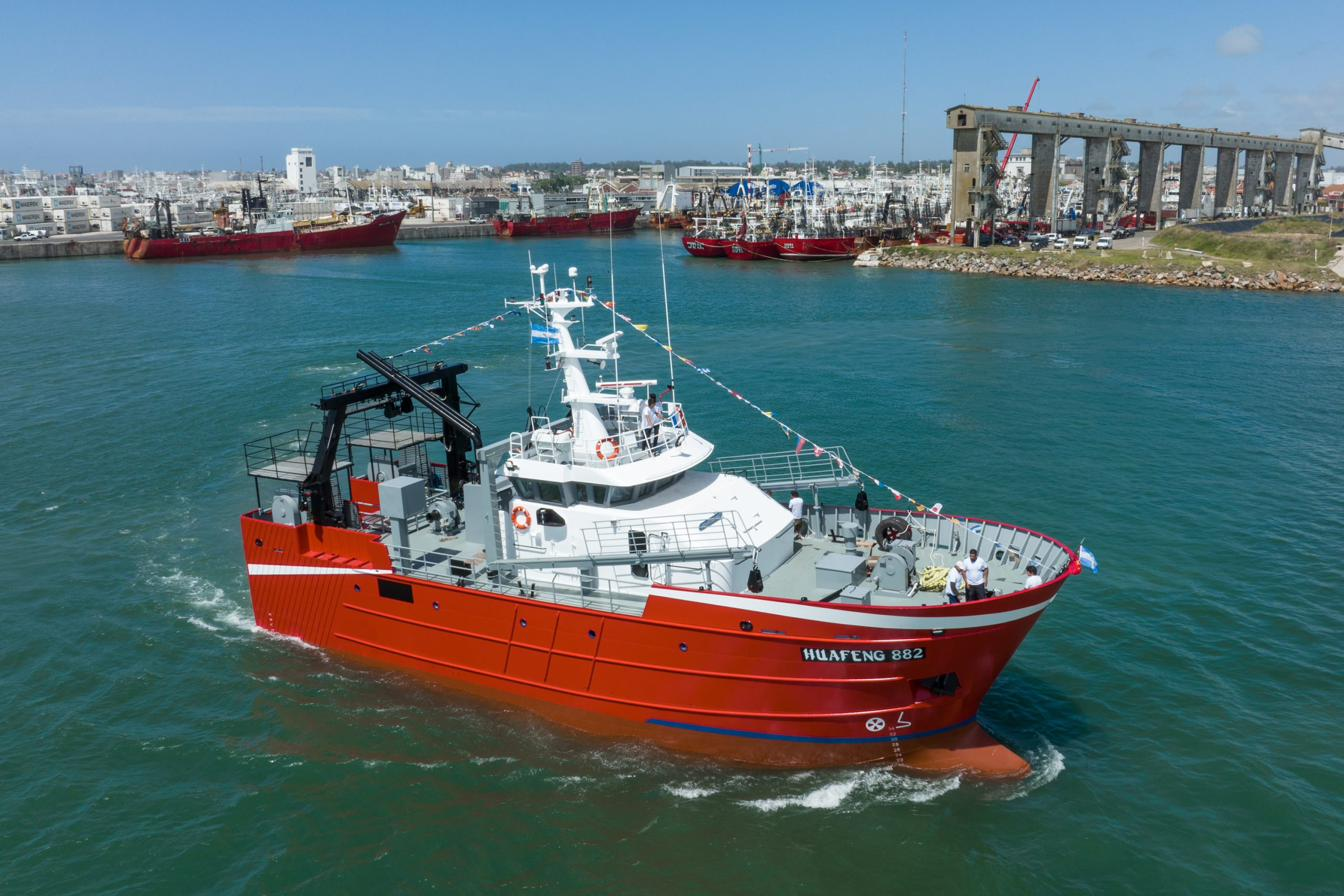
\includegraphics[width=\linewidth]{pesquero_real.jpg}
\column{0.50\textwidth}
  \begin{itemize}
    \item La pesca es uno de los principales complejos exportadores del país: \alert{USD 2010 M} en 2025.
    \item Proceso de \alert{renovación de flota} con buques construidos íntegramente en astilleros nacionales.
    \item Tipología de \alert{baja esbeltez}: $L/B<4$, popa llena, dormido pronunciado.
    \item La predicción de potencia se apoya en métodos de extrapolación modelo–buque desarrollados y validados sobre \alert{mercantes esbeltos}.
  \end{itemize}
\end{columns}
\mensaje{¿Son válidos esos métodos para cascos de baja esbeltez?}
\note{1 min. No detenerse en la historia de la pesca. La pregunta del recuadro es la motivación particular; la siguiente diapositiva es la motivación general.}
\end{frame}

\begin{frame}{El origen del problema: semejanza dinámica parcial}
Con el mismo fluido y la misma gravedad, el modelo \alert{no puede igualar a la vez} Froude y Reynolds.
\vspace{0.6em}
\begin{columns}[T]
\column{0.48\textwidth}
\begin{block}{Resistencia al avance}
\small
$Fr_M = Fr_S \;\Rightarrow\; Re_M \approx Re_S/\lambda^{3/2}$\\[2pt]
Hipótesis de Hughes (ITTC-78):
\[C_{TS} = \uk\,C_{F0}(Re_S) + C_W\]
Supuesto: \alert{$k_M = k_S$}, el factor de forma no depende de la escala.\\[2pt]
\Pu{} ($\lambda=20$): $Re_S/Re_M \approx 90$.
\end{block}
\column{0.48\textwidth}
\begin{block}{Propulsión (aguas abiertas)}
\small
$J_M = J_S$ con $Re_M \ll Re_S$\\[2pt]
Procedimiento ITTC-78 para hélices:
\[K_{TS} = K_{TM} - \Delta K_T,\quad \Delta K_T = -\Delta C_D\,0.3\,\tfrac{P}{D}\tfrac{c\,Z}{D}\]
Corrección de \alert{fricción de placa plana}: implícitamente $\Delta K_{Tp}=0$.
\end{block}
\end{columns}
\mensaje{Ambos procedimientos tratan el efecto de escala como esencialmente \textbf{friccional}.}
\note{1,5 min. Esta es la idea que vuelve al final: los métodos vigentes corrigen fricción. Remarcar el factor 90 en Reynolds para el P1.}
\end{frame}

\begin{frame}{Por qué estos dos ejes}
El Comité de Métodos Combinados CFD/EFD de la \textbf{29.ª ITTC} relevó los problemas de escala en la predicción de potencia y propuso concentrar esfuerzos en cinco temas. Dos de ellos son los ejes de esta tesis:
\vspace{0.8em}
\begin{columns}[T]
\column{0.48\textwidth}
\begin{dato}[title={\textbf{Eje 1 · Determinación numérica de $\uk$}},colbacktitle=mar,coltitle=white]
\small
\begin{itemize}
  \item Calificación \alert{más alta} de todos los temas evaluados.
  \item Prohaska puede fallar: errores del orden del 5\,\% y de hasta \alert{10\,\% en la potencia total}.
  \item Puede distorsionar tendencias de diseño.
\end{itemize}
\end{dato}
\column{0.48\textwidth}
\begin{dato}[title={\textbf{Eje 2 · Escalado de hélices en aguas abiertas}},colbacktitle=mar,coltitle=white]
\small
\begin{itemize}
  \item Mejora de los métodos de escalado de ensayos POW.
  \item Régimen completamente turbulento y \alert{transición} a escala de modelo.
\end{itemize}
\end{dato}
\end{columns}
\vfill
\fuente{ITTC (2021). Final Report and Recommendations to the 29th ITTC — Specialist Committee on Combined CFD/EFD Methods.}
\note{1 min. Esto justifica la elección de los ejes con una referencia externa: no es una elección arbitraria.}
\end{frame}

\begin{frame}{Objetivos e hilo conductor}
\begin{columns}[T]
\column{0.48\textwidth}
\begin{block}{Eje 1 — Resistencia: factor de forma}
\small Caracterizar, mediante EFD–CFD, los efectos de escala en la determinación de $\uk$ y su influencia en la predicción de resistencia, con foco en \alert{pesqueros de baja esbeltez}.
\end{block}
\column{0.48\textwidth}
\begin{block}{Eje 2 — Propulsión: hélices}
\small Caracterizar, mediante EFD–CFD, los efectos de escala en hélices en aguas abiertas, en régimen \alert{turbulento} y con \alert{transición} laminar–turbulenta a escala de modelo.
\end{block}
\end{columns}
\vspace{1em}
\begin{alertblock}{Pregunta transversal}
¿Qué parte del efecto de escala es \textbf{fricción} y qué parte es \textbf{presión}?
\end{alertblock}
\vspace{0.4em}
\small Estrategia: el \textbf{ensayo} valida la herramienta en el régimen accesible; el \textbf{CFD} validado extiende el análisis a escala buque y \alert{descompone las fuerzas}.
\note{1 min. Anunciar el hilo conductor: lo vamos a responder dos veces, una por eje.}
\end{frame}

% =====================================================================
\section{Antecedentes}
\note{Bloque objetivo: \textbf{3 min}. El jurado conoce el tema: solo lo necesario para entender los resultados.}
% =====================================================================

\begin{frame}{El método de Prohaska y sus limitaciones}
\begin{columns}[T]
\column{0.48\textwidth}
  \centering
  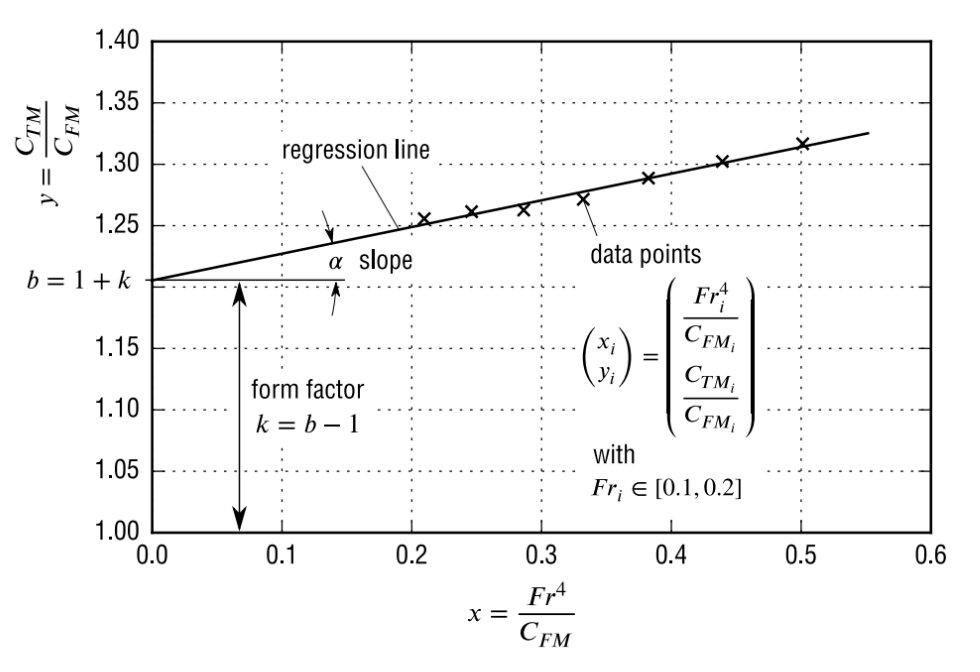
\includegraphics[width=0.66\linewidth]{prohaska_diagram.png}\\
  \fuente{Adaptado de Birk (2019).}
  \[\frac{C_{TM}}{C_{F0}} = \uk + c\,\frac{Fr^4}{C_{F0}},\qquad 0.1<Fr<0.2\]
\column{0.48\textwidth}
  \centering
  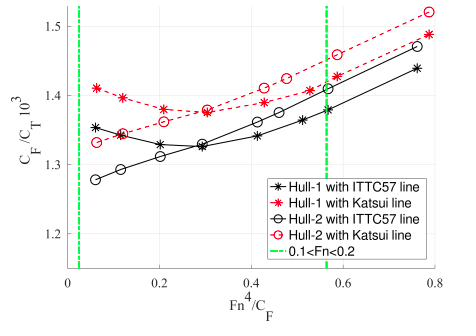
\includegraphics[width=0.62\linewidth]{prohaska-korkmaz-a.png}\\
  \fuente{Adaptado de Korkmaz et al. (2021).}
  \begin{itemize}\small
    \item Supone flujo adherido y $C_W\propto Fr^4$ a baja velocidad.
    \item Se desvía con: \alert{proa bulbo} cerca de la superficie, \alert{separación} / popa espejo sumergida, y la \alert{línea de referencia}.
  \end{itemize}
\end{columns}
\mensaje{Las tres fuentes de desviación están presentes en los pesqueros estudiados.}
\note{1 min. Anticipa la estructura del Eje 1: bulbo, popa sumergida y línea de fricción se analizan como causas alternativas.}
\end{frame}

\begin{frame}{El factor de forma depende de la escala}
\begin{columns}[c]
\column{0.36\textwidth}
  \centering
  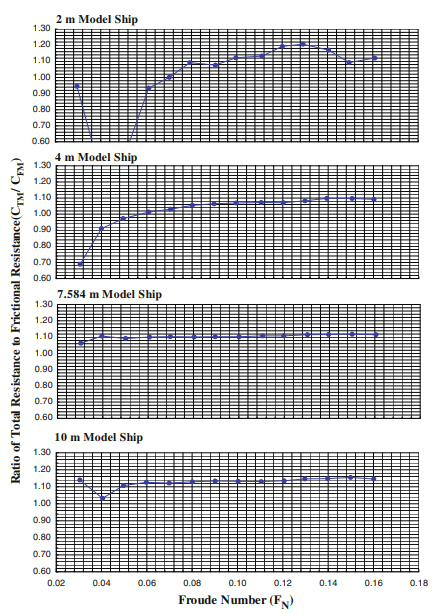
\includegraphics[height=4.9cm]{keh-sik-min.png}\\
  \fuente{Geosims de un portacontenedores. Min y Kang (2010).}
\column{0.60\textwidth}
  \begin{itemize}
    \item Ensayos con geosims y CFD en doble cuerpo muestran $\uk$ \alert{creciente con Re} (Min y Kang, 2010; Terziev et al., 2021).
    \item Dos contribuciones: la \alert{línea de referencia} (ITTC-57 no es una placa plana pura) y la \alert{física asociada a la forma} del casco.
    \item Correlaciones de corrección (p. ej. García-Gómez, 2000) calibradas en cascos con $L/B \approx 7$–$9$.
    \item Prácticamente \alert{sin datos para $L/B<4$}.
  \end{itemize}
\end{columns}
\mensaje{Vacío: el efecto de escala de $\uk$ en cascos de baja esbeltez no estaba caracterizado.}
\note{1 min.}
\end{frame}

\begin{frame}{Hélices: el supuesto friccional del ITTC-78}
\begin{columns}[c]
\column{0.50\textwidth}
  \begin{itemize}
    \item Ensayos POW a $Re_{c,0.7R}\sim 2\times10^5$–$2\times10^6$: capa límite \alert{transicional}.
    \item $K_T$, $K_Q$ no monótonos con $Re$: “\alert{joroba}” que un modelo completamente turbulento no captura.
    \item El ITTC-78 corrige solo $\Delta C_D$: no contempla \alert{redistribución de presión} ni transición.
    \item Trabajos CFD recientes apuntan a un efecto de escala con componente de presión relevante (Gaggero, 2026; Gallotti y Gaggero, 2026).
  \end{itemize}
\column{0.47\textwidth}
  \centering
  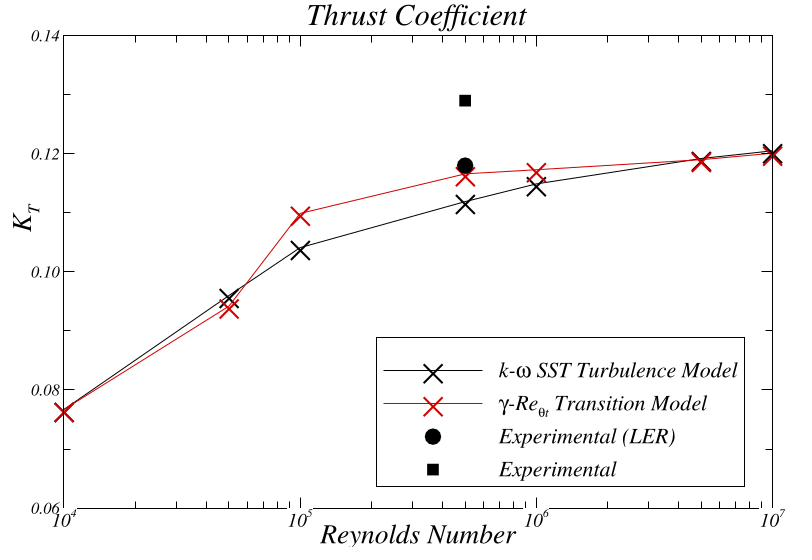
\includegraphics[width=\linewidth]{joroba_kt_joao.png}\\
  \fuente{Adaptado de Baltazar et al. (2018).}
\end{columns}
\note{1 min.}
\end{frame}

% =====================================================================
\section{Metodología EFD--CFD}
\note{Bloque objetivo: \textbf{6 min}.}
% =====================================================================

\begin{frame}{Casos de estudio: cuatro cascos ensayados en el LabHiNO}
\centering
{\setlength{\tabcolsep}{3pt}\begin{tabular}{cccc}
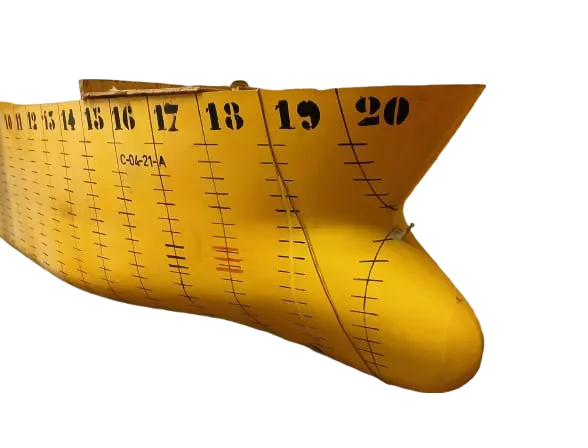
\includegraphics[height=2.05cm]{tpa-pers.png} &
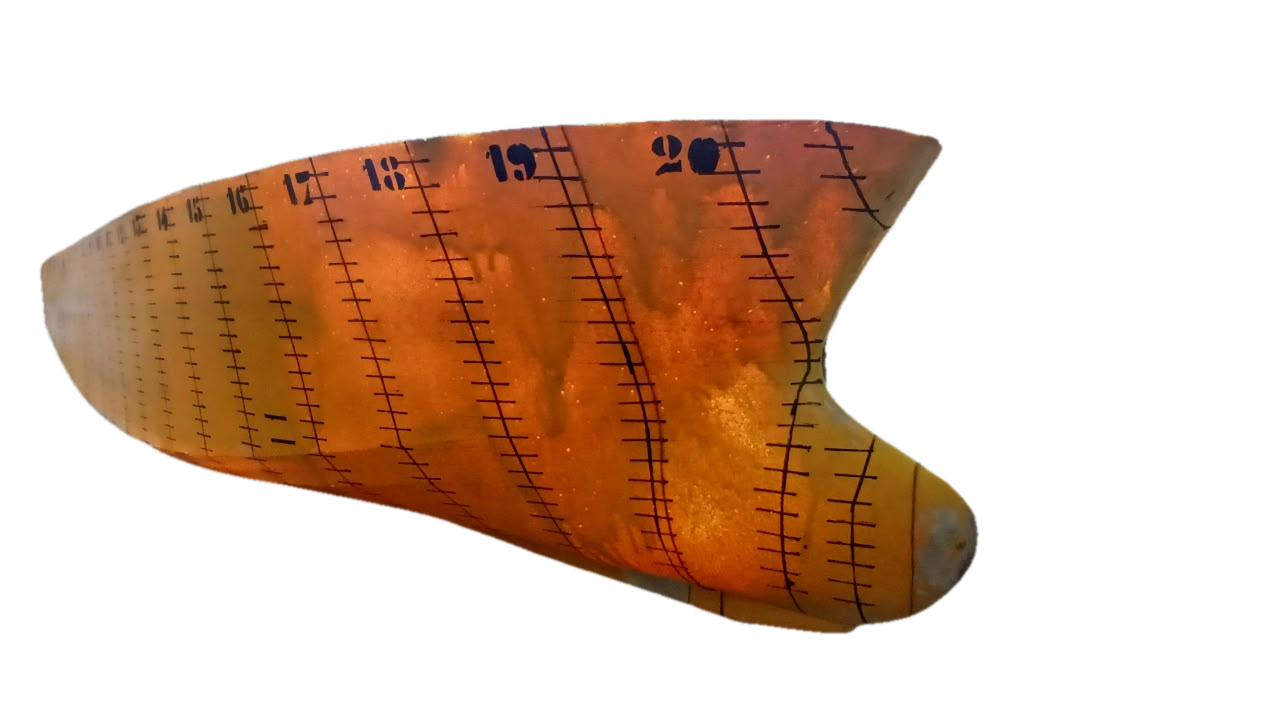
\includegraphics[height=2.05cm]{contessi-pers.png} &
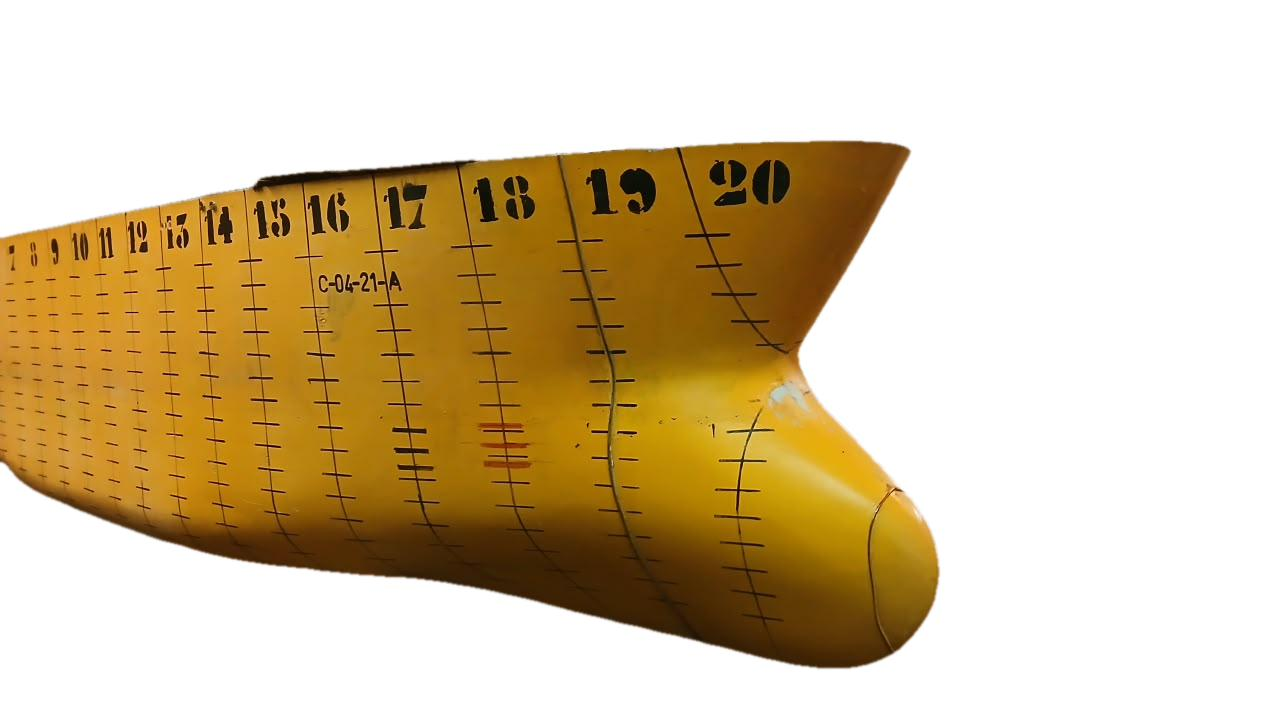
\includegraphics[height=2.05cm]{jpa-pers.png} &
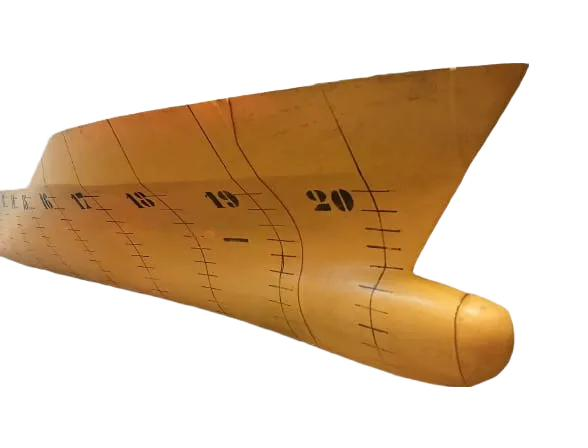
\includegraphics[height=2.05cm]{kcs-pers.png} \\
\small\Pu & \small\Pd & \small\Pt & \small\KCS
\end{tabular}}
\vspace{0.5em}

\small
\begin{tabular}{lccccl}
\toprule
Casco & $\lambda$ & $L_{WL}$ [m] & $B$ [m] & $L/B$ & Ensayos \\
\midrule
\Pu  & 20 & 32.68 & 9.28 & \alert{3.52} & 3 calados; variantes con/sin bulbo \\
\Pd  & 10 & 25.10 & 7.80 & \alert{3.22} & 1 calado \\
\Pt  & 13 & 22.05 & 7.80 & \alert{2.83} & 1 calado \\
\KCS & 79 & 230.0 & 32.2 & 7.14 & referencia esbelta (base de datos internacional) \\
\bottomrule
\end{tabular}
\note{1 min. Tres pesqueros reales de astilleros nacionales y el KCS como contraste. El P1 es el caso estudiado en profundidad.}
\end{frame}

\begin{frame}{Metodología experimental (EFD)}
\begin{columns}[T]
\column{0.49\textwidth}
  \centering
  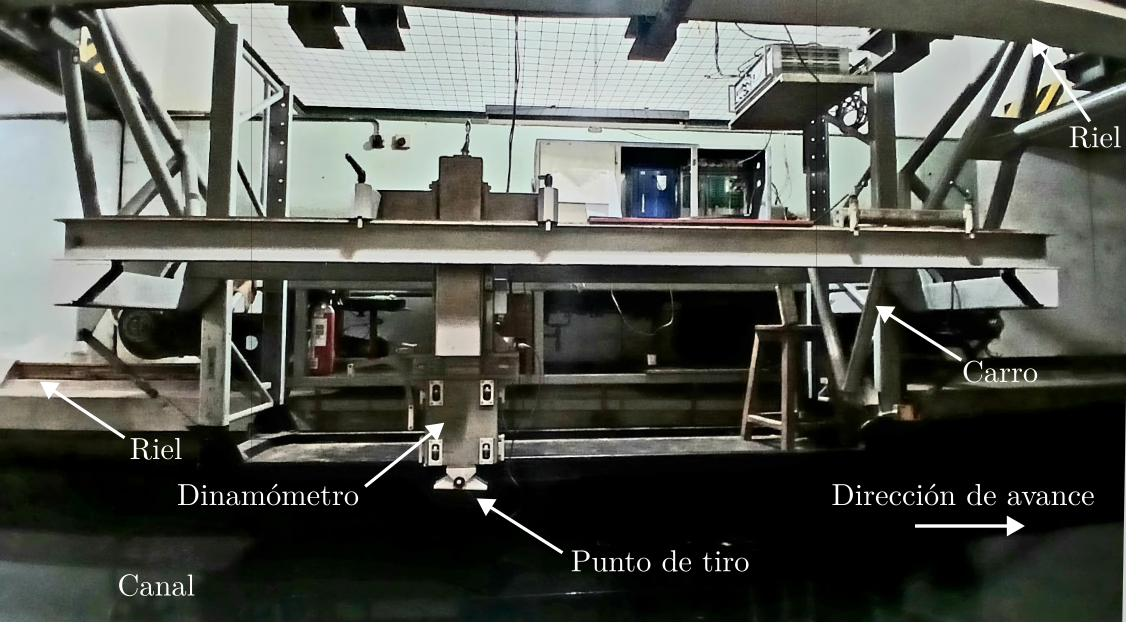
\includegraphics[height=3.3cm]{esquema_resistencia.png}
  \begin{itemize}\small
    \item Canal de remolque LabHiNO: 72\,m $\times$ 3.6\,m $\times$ 2.0\,m; carro hasta 4\,m/s.
    \item Modelo libre en cabeceo y hundimiento; estimuladores de turbulencia a 5\,\% $L$.
    \item Incertidumbre según ITTC (RSS) y ajuste ponderado de \alert{York} sobre Prohaska.
  \end{itemize}
\column{0.49\textwidth}
  \centering
  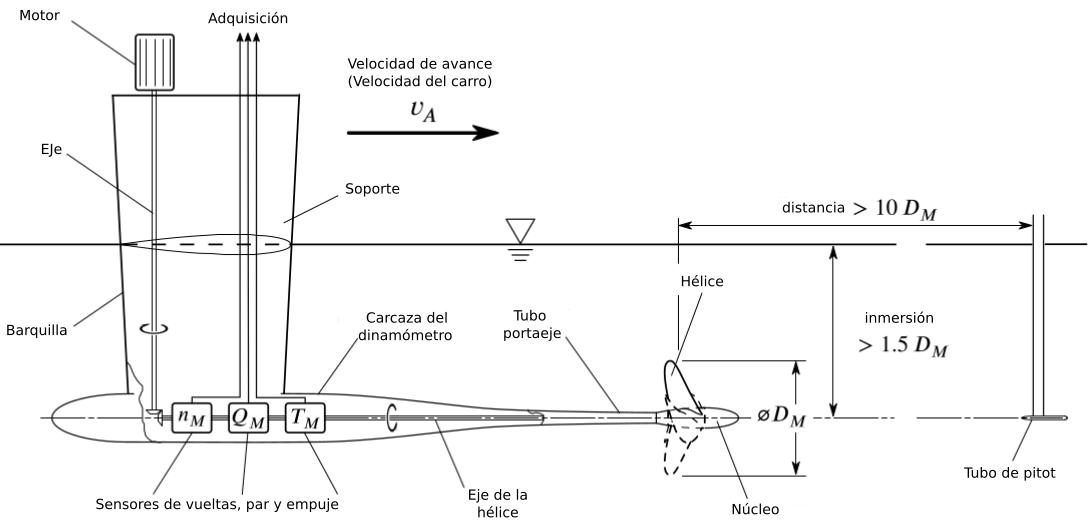
\includegraphics[height=3.3cm]{esquema_aguas_abiertas.png}
  \begin{itemize}\small
    \item \Bfs: ensayos de archivo del LabHiNO ($D=0.14$\,m) y polinomios MARIN.
    \item \Pdos: túnel de cavitación (datos del fabricante), \alert{5 velocidades de giro} $\Rightarrow$ 5 números de Reynolds.
  \end{itemize}
\end{columns}
\note{1 min. Mencionar que parte de los datos son propios y parte preexistentes o cedidos.}
\end{frame}

\begin{frame}{Metodología numérica: casco}
\begin{columns}[T]
\column{0.45\textwidth}
  \centering
  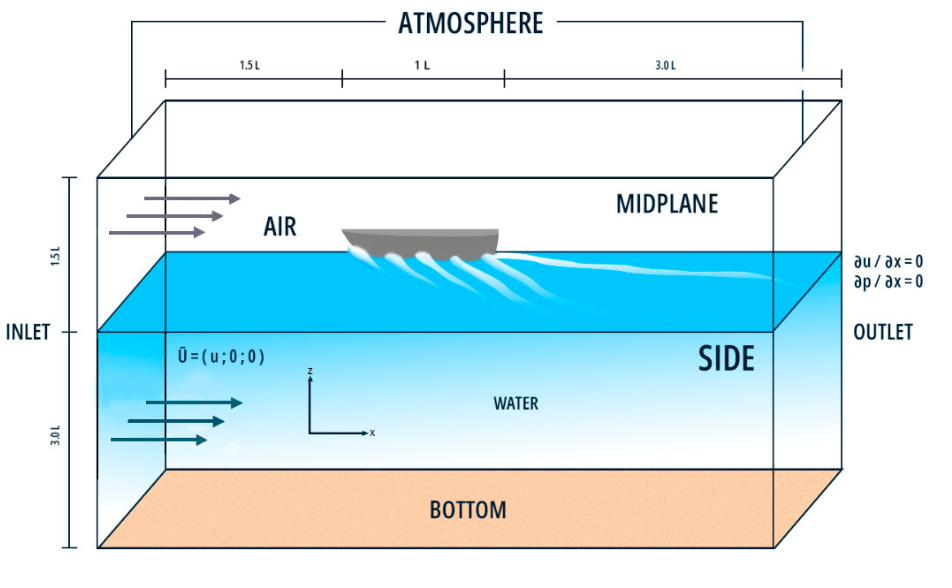
\includegraphics[width=0.95\linewidth]{domain.png}\\[4pt]
  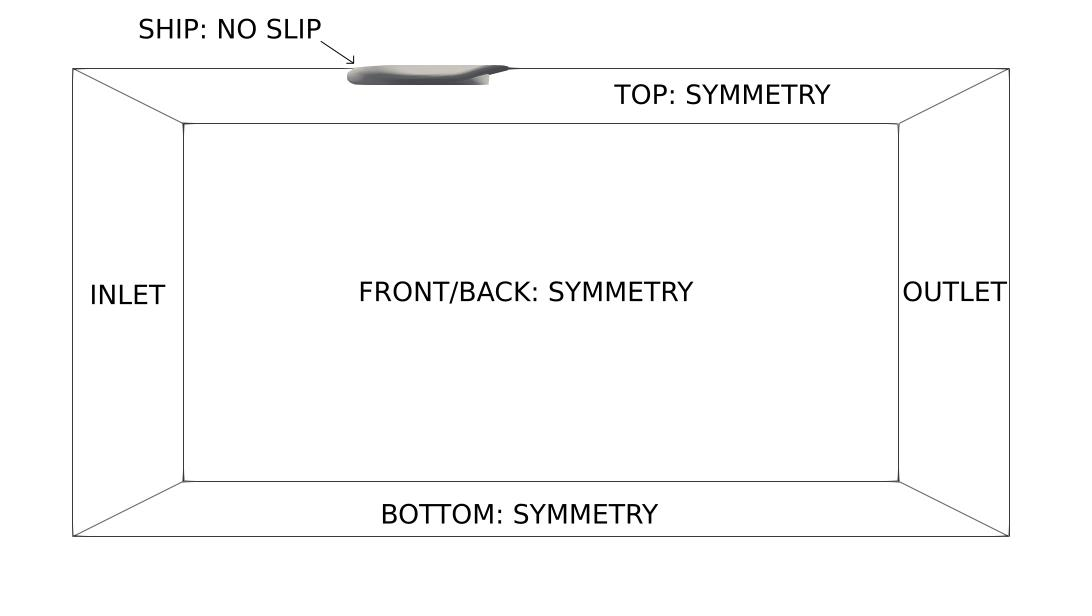
\includegraphics[width=0.80\linewidth]{esquema_malla.png}
\column{0.53\textwidth}
  \begin{itemize}\small
    \item OpenFOAM 11, RANS $k$–$\omega$ SST; malla hexaédrica (\texttt{snappyHexMesh}) con capas prismáticas.
    \item \textbf{Con superficie libre} (\texttt{interFoam}, VoF): replica el ensayo para validar.
    \item \textbf{Doble cuerpo (DB)}: sin olas, por lo que
    \[C_T = C_V \;\Rightarrow\; \uk = \frac{C_V}{C_{F0}}\ \text{ a cada } Re\]
    \item Geosims \alert{1:20, 1:10, 1:5 y 1:1}: barrido de Reynolds hasta escala buque.
    \item Descomposición: $C_V = C_F + C_{PV}$, inaccesible en el ensayo.
  \end{itemize}
\end{columns}
\note{1,5 min. El DB es la herramienta central del Eje 1: da k a cualquier escala, sin el sesgo de la regresión de Prohaska.}
\end{frame}

\begin{frame}{Metodología numérica: hélice y verificación–validación}
\begin{columns}[T]
\column{0.40\textwidth}
  \centering
  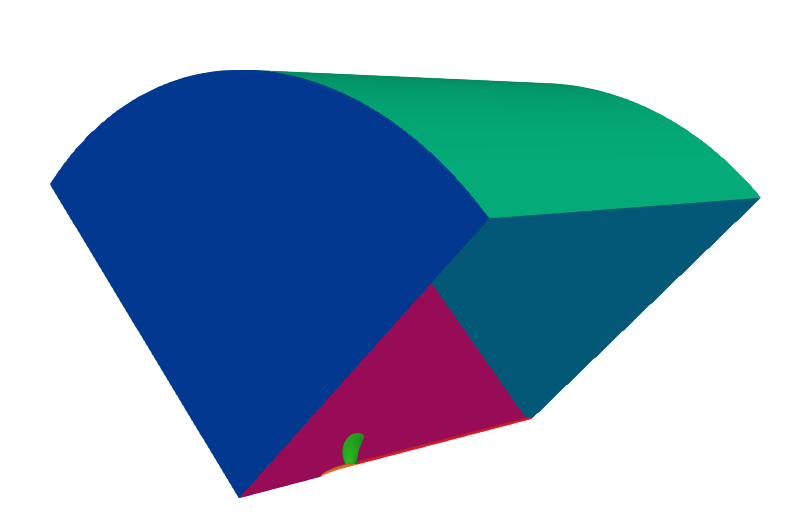
\includegraphics[width=0.95\linewidth]{fig_helice_dominio.png}
\column{0.58\textwidth}
  \begin{itemize}\small
    \item Formulación MRF; \alert{OpenFOAM y StarCCM+}.
    \item $k$–$\omega$ SST (completamente turbulento) y SST-LM $\gamma$–$\widetilde{Re}_{\theta t}$ (transición), con la intensidad turbulenta $Tu$ como parámetro.
    \item \Bfs: barrido geométrico $D = 0.14$–$8.0$\,m a $J$ constante.
    \item Descomposición directa: $K_T = K_{Tp} + K_{Tf}$, $K_Q = K_{Qp}+K_{Qf}$.
  \end{itemize}
  \begin{block}{V\&V (procedimientos ITTC)}
  \small
  Convergencia de malla con \textbf{GCI} (tres mallas). Validación: error $E\%D$ frente a
  $U_{val} = \sqrt{U_D^2 + U_{num}^2}$.
  \end{block}
\end{columns}
\note{1,5 min. Si preguntan por y+: en casco va de ~1 a escala modelo a >300 a escala buque, con funciones de pared adaptativas (respaldo).}
\end{frame}

% =====================================================================
\section{Eje 1: resistencia al avance y factor de forma}
\note{Bloque objetivo: \textbf{17 min}. Es el corazón de la defensa.}
% =====================================================================

\begin{frame}{EFD: el \KCS{} cumple Prohaska; el pesquero no}
\begin{columns}[T]
\column{0.49\textwidth}
  \centering
  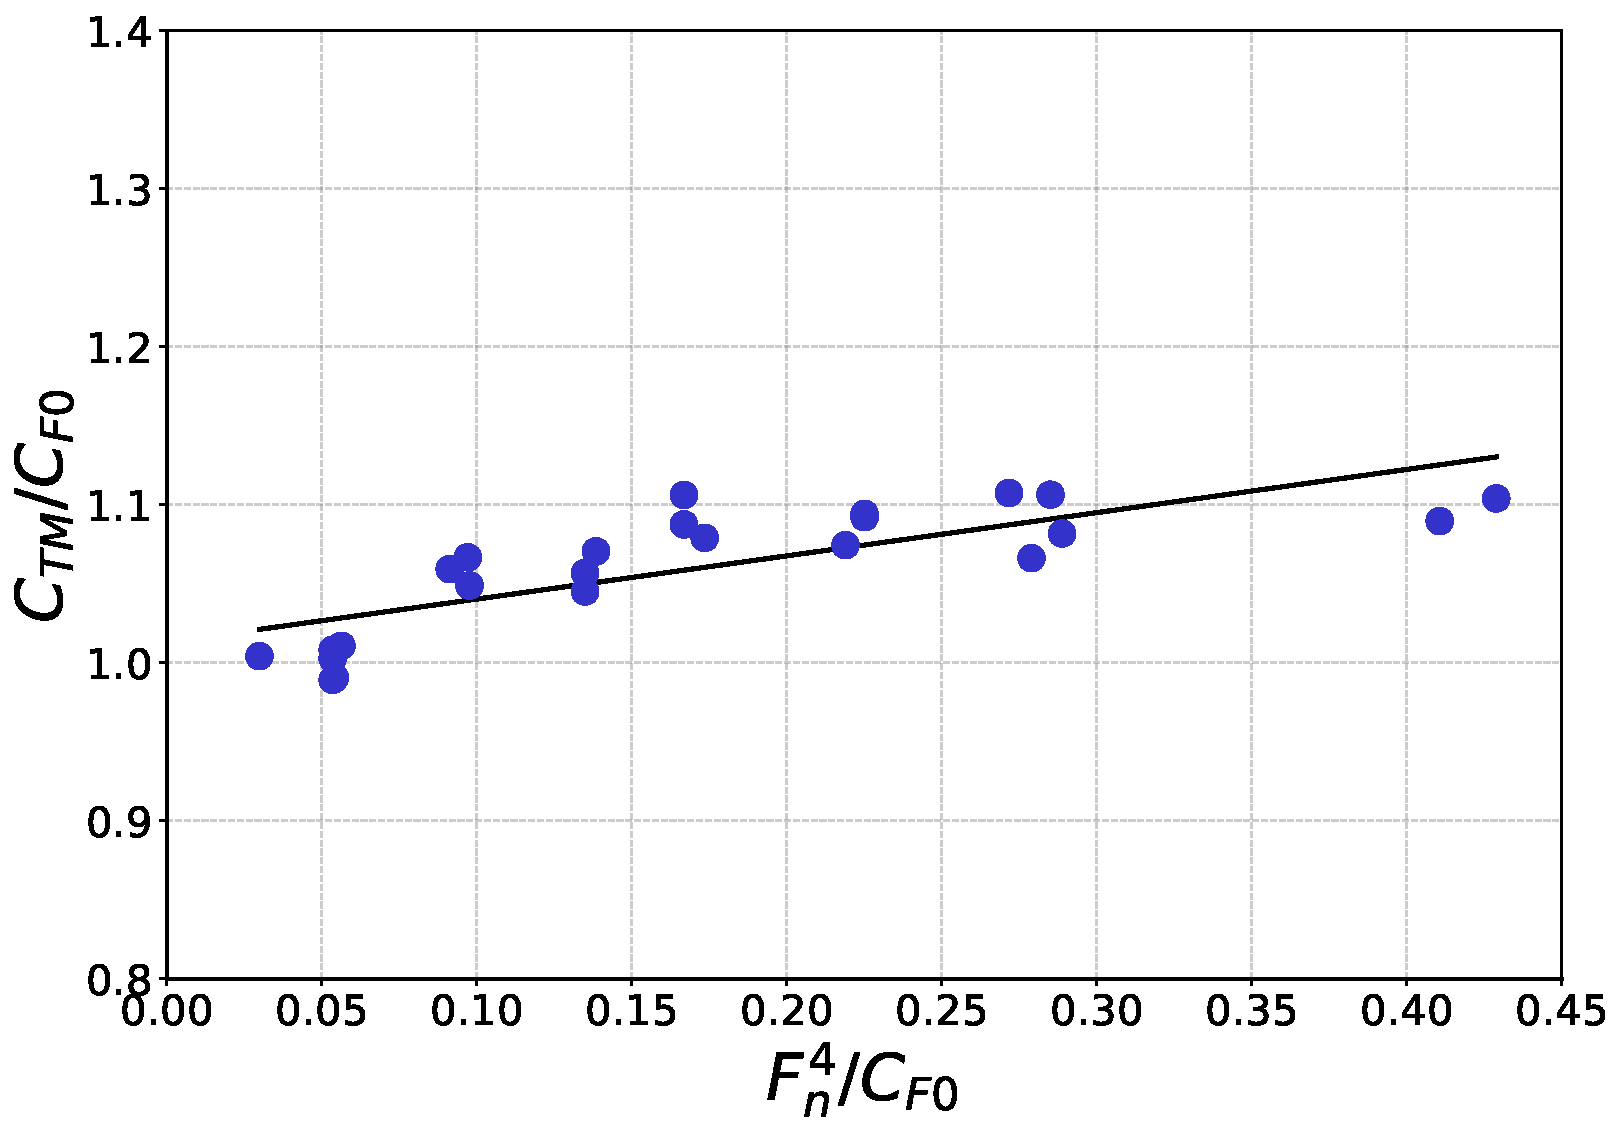
\includegraphics[width=0.84\linewidth]{prohaska_kcs.pdf}\\
  \small \KCS: puntos alineados sobre la recta.\\
  $\uk = 1.052 \pm 2.3\,\%$
\column{0.49\textwidth}
  \centering
  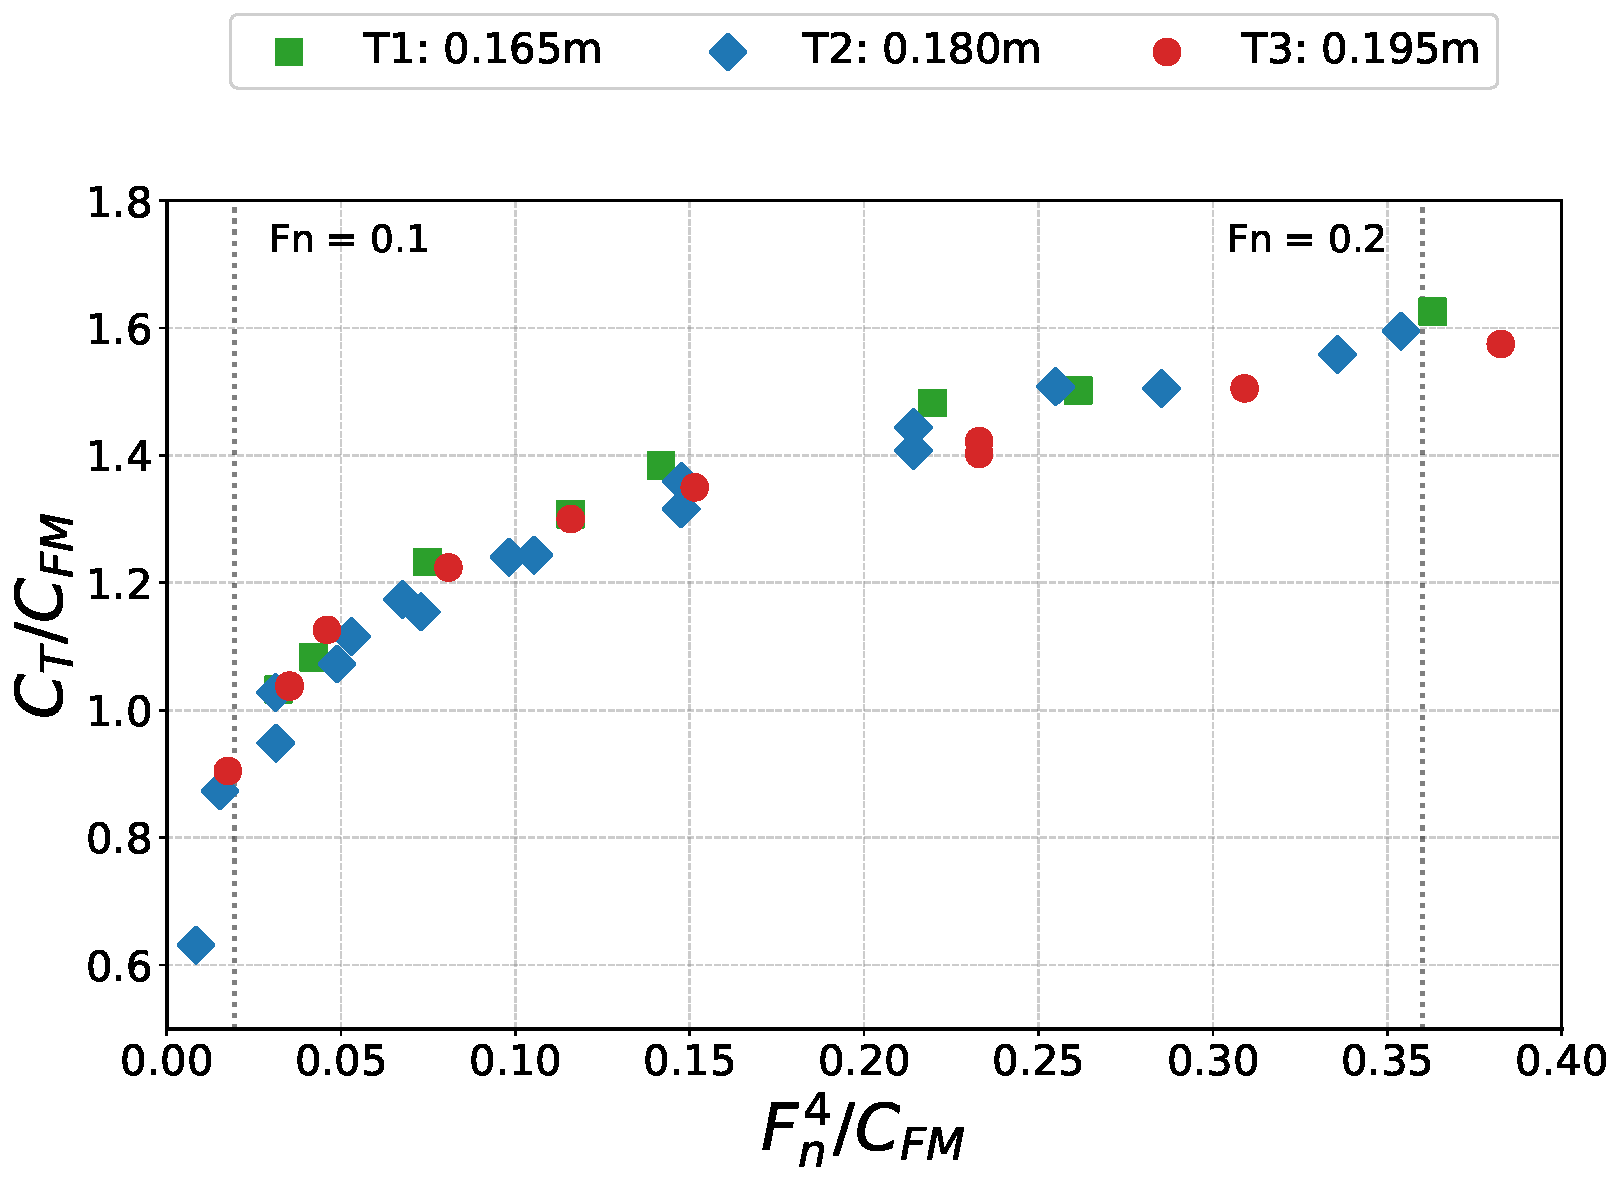
\includegraphics[width=0.84\linewidth]{prohaska_tpa_comparacion.pdf}\\
  \small \Pu, tres calados: \alert{curvatura sistemática} a bajo $Fr$.\\
  $\uk = 1.19$–$1.24 \pm$ \alert{8–11\,\%}
\end{columns}
\mensaje{Primera asimetría: los supuestos del método se cumplen con mucha menos holgura en el casco de baja esbeltez.}
\note{1,5 min. Incertidumbres obtenidas con ajuste de York. La curvatura anticipa que algo no lineal ocurre a bajo Fr.}
\end{frame}

\begin{frame}{Validación EFD–CFD con superficie libre (\Pu, calado T2)}
\begin{columns}[c]
\column{0.50\textwidth}
  \centering
  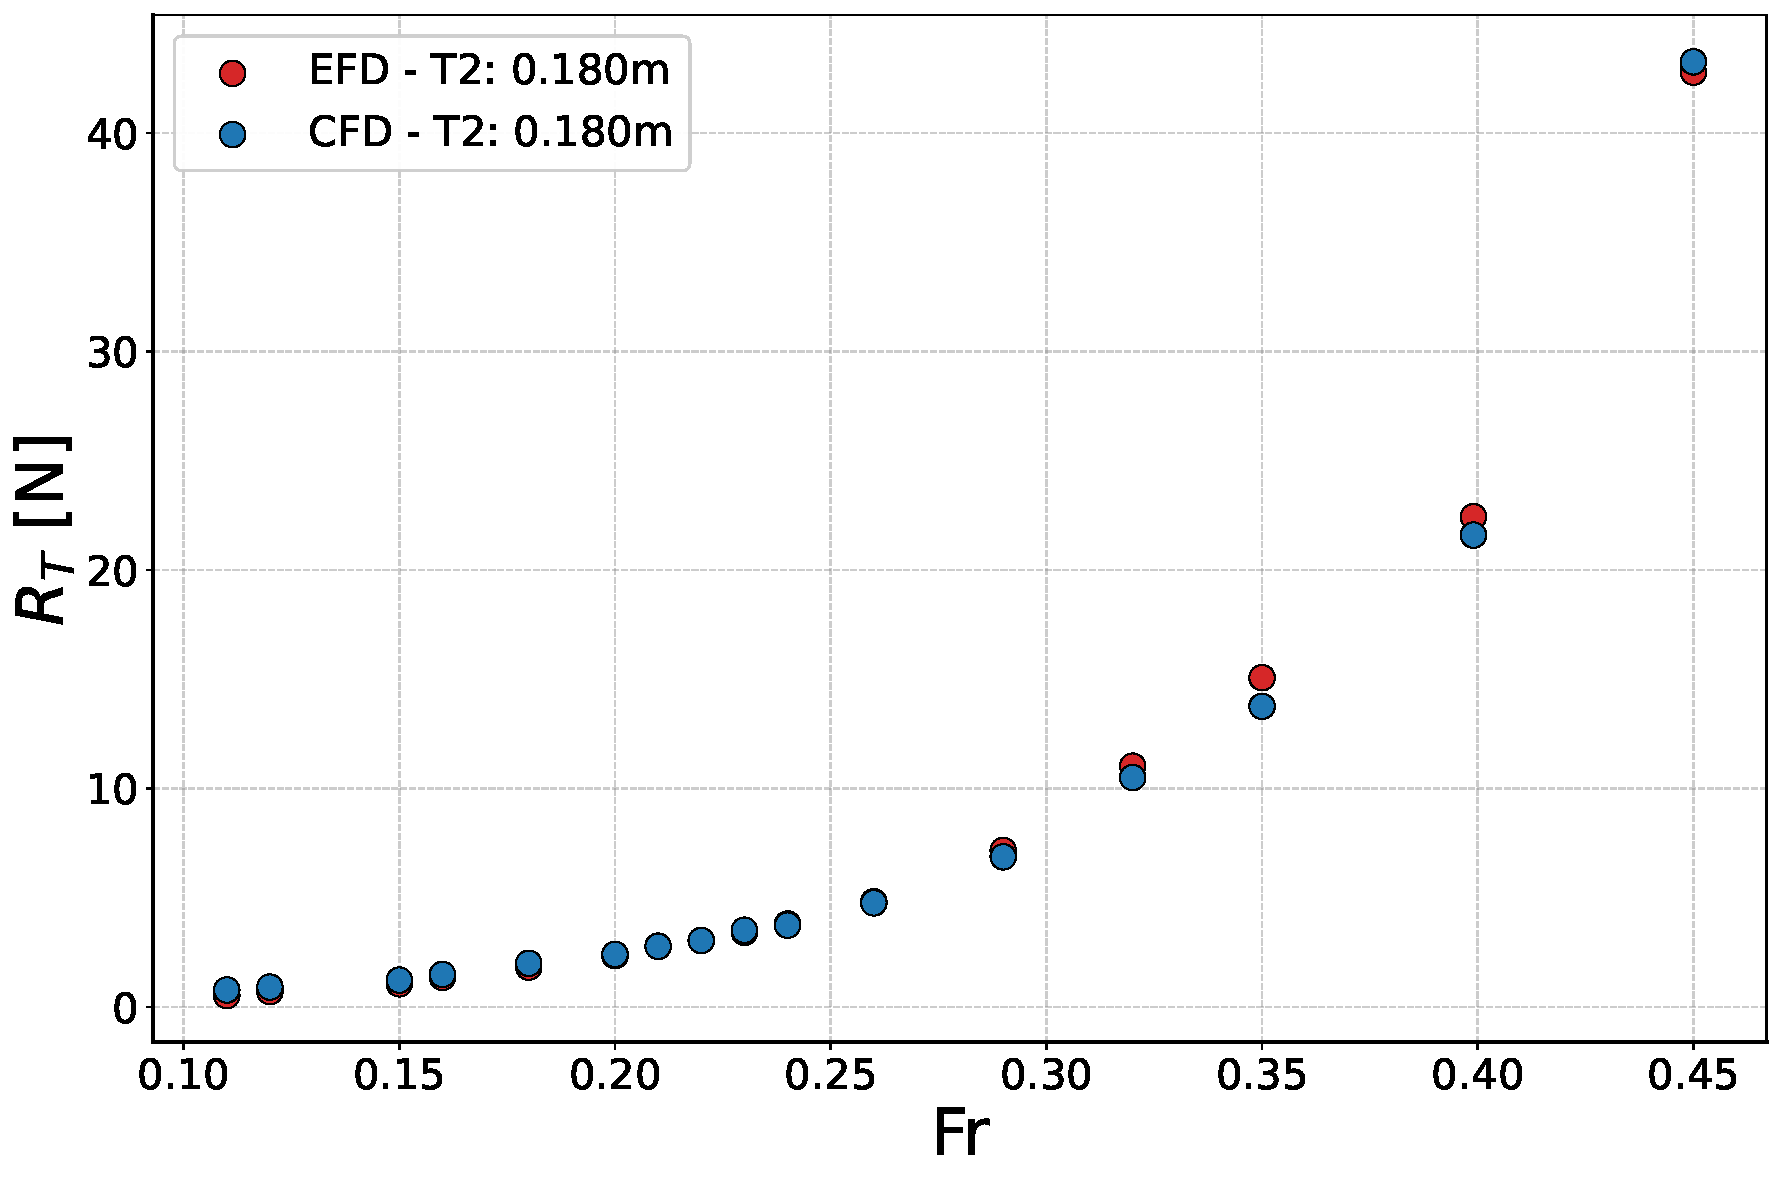
\includegraphics[width=\linewidth]{efd_cfd_180.pdf}
\column{0.48\textwidth}
  \centering\small
  \begin{tabular}{cccc}
  \toprule
  $Fr$ & $E\%D$ & $U_{val}$ [\%] & ¿Validado? \\
  \midrule
  0.20 & $-2.4$ & 3.7 & Sí \\
  0.22 & $-0.1$ & 3.1 & Sí \\
  0.24 & $\phantom{-}1.3$ & 2.6 & Sí \\
  0.26 & $\phantom{-}1.0$ & 2.0 & Sí \\
  0.29 & $\phantom{-}4.1$ & 1.7 & \alert{No} \\
  0.32 & $\phantom{-}4.7$ & 1.4 & \alert{No} \\
  \bottomrule
  \end{tabular}
  \vspace{0.6em}
  \begin{itemize}\small
    \item Validado en el \alert{rango operativo} ($Fr\le0.26$).
    \item A $Fr\ge0.29$: el CFD fija cabeceo y hundimiento; el ensayo no.
    \item Otros calados: $\sim$5\,\% (T1) y 1–2\,\% (T3).
  \end{itemize}
\end{columns}
\note{1,5 min. U\_num < 0,2 \%, despreciable frente a U\_D.}
\end{frame}

\begin{frame}{El doble cuerpo reproduce el $\uk$ experimental a bajo $Fr$}
\begin{columns}[c]
\column{0.50\textwidth}
  \centering
  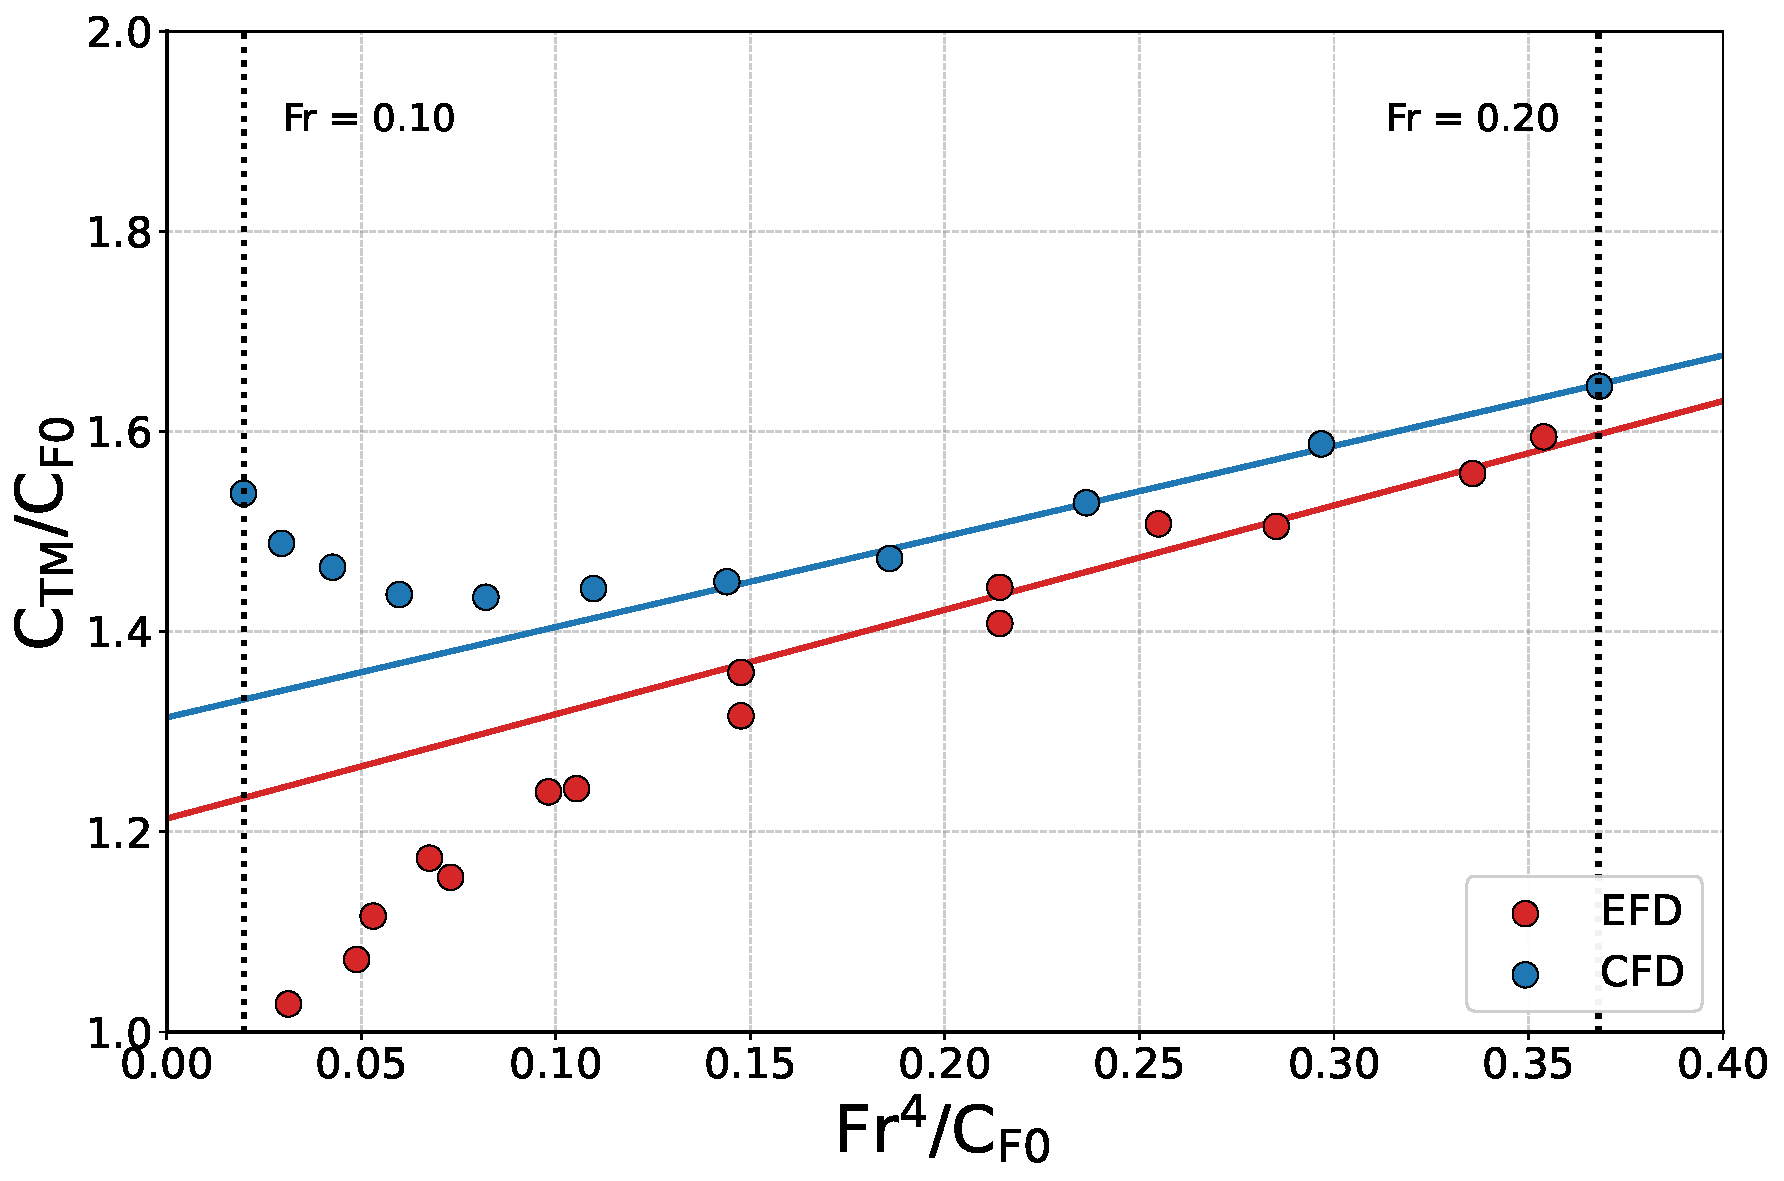
\includegraphics[width=\linewidth]{prohaska-efd-cfd-180.pdf}\\
  \fuente{Diagrama de Prohaska EFD y CFD, calado T2.}
\column{0.48\textwidth}
  \centering\small
  \begin{tabular}{lccc}
  \toprule
  & T1 & T2 & T3 \\
  \midrule
  DB, $Fr=0.10$ & 1.168 & 1.157 & 1.179 \\
  DB, $Fr=0.16$ & 1.233 & 1.225 & 1.251 \\
  \midrule
  Prohaska EFD & 1.235 & 1.195 & 1.193 \\
  \quad $U_{1+k}$ & $\pm0.104$ & $\pm0.129$ & $\pm0.133$ \\
  Prohaska CFD & 1.193 & 1.314 & 1.254 \\
  \bottomrule
  \end{tabular}
  \vspace{0.6em}
  \begin{itemize}\small
    \item El DB cae dentro de la incertidumbre del Prohaska experimental.
    \item Respalda usar el DB para \alert{extender el análisis a escala buque}.
  \end{itemize}
\end{columns}
\note{1 min. Matiz honesto: el DB no tiene contraparte experimental directa; esto es evidencia indirecta, condición necesaria.}
\end{frame}

\begin{frame}{Resultado central: el $\uk$ del pesquero no se estabiliza}
\begin{columns}[c]
\column{0.64\textwidth}
  \centering
  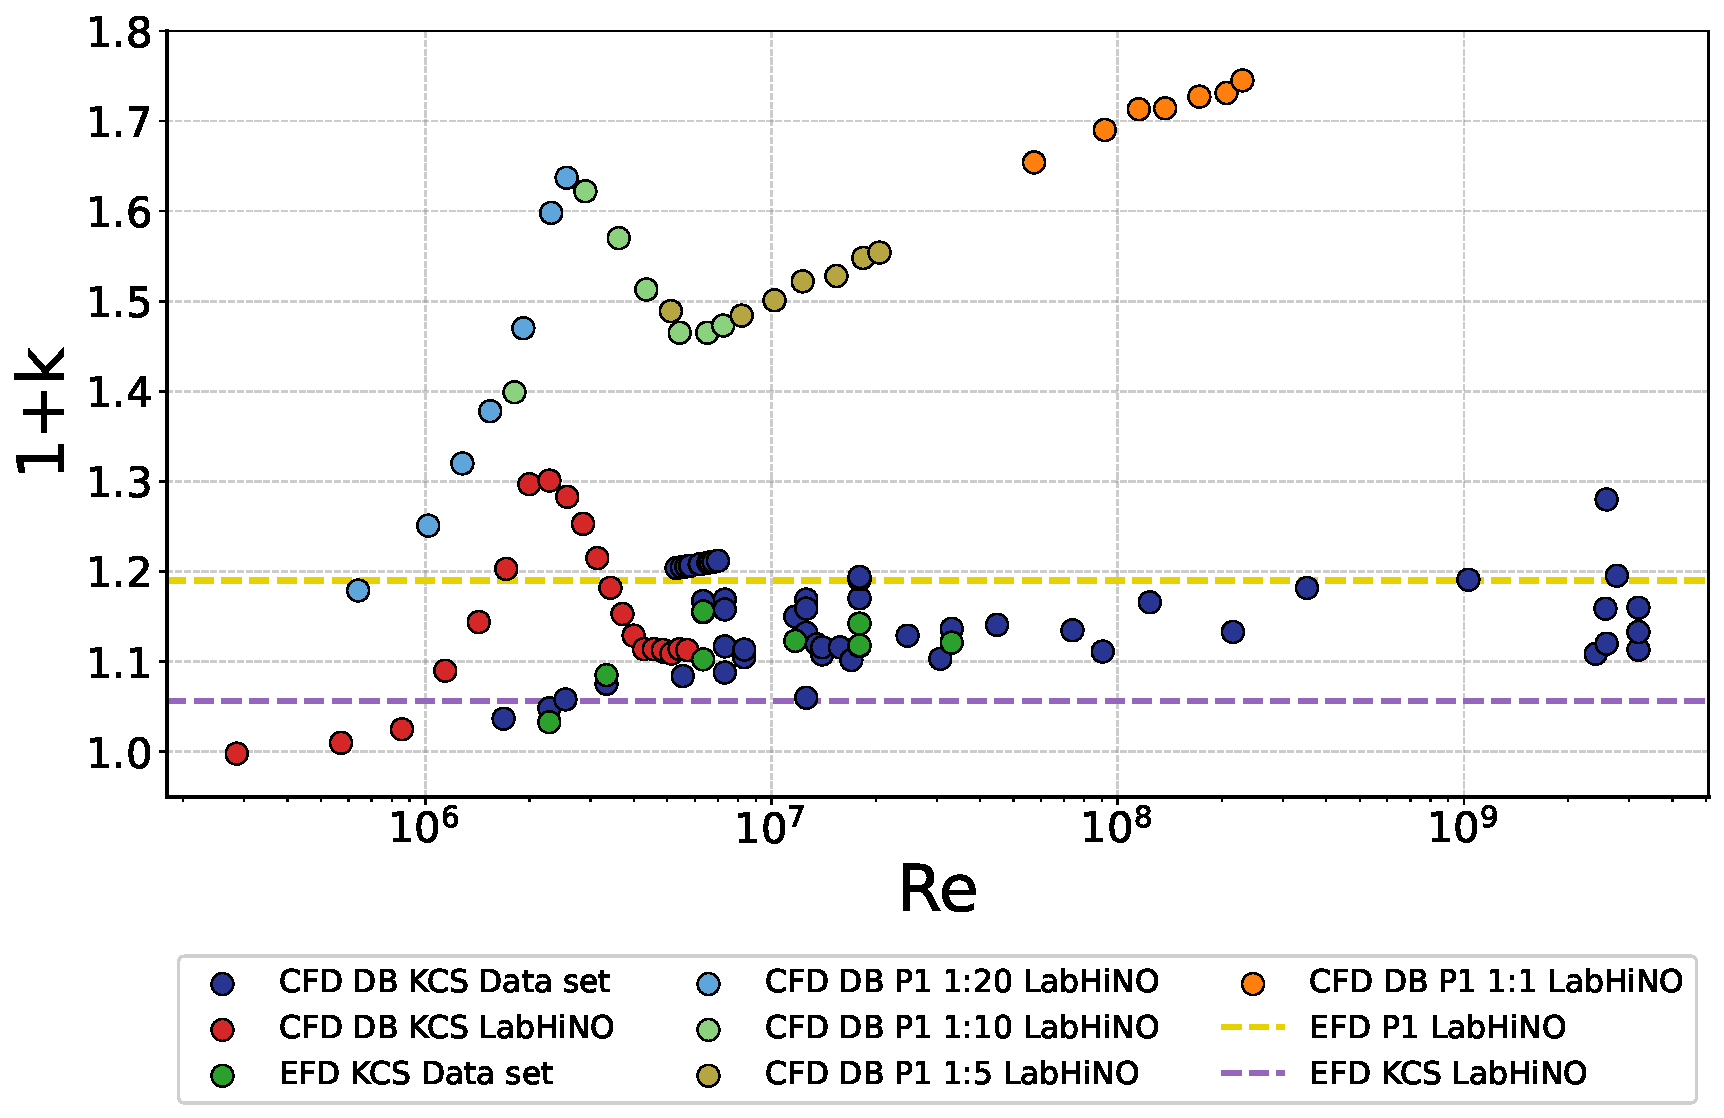
\includegraphics[width=0.90\linewidth]{completo_log_kcs_lit_tpa.pdf}
\column{0.34\textwidth}
  \begin{dato}[title={\KCS},colbacktitle=gris,coltitle=white]
  \footnotesize Crece y \textbf{se estabiliza}, como predice la teoría.\\
  Bajo vs. alto $Re$: $\approx$ \textbf{8\,\%}
  \end{dato}
  \vspace{0.3em}
  \begin{dato}[title={\Pu},colbacktitle=acento,coltitle=white]
  \footnotesize Crece de forma \textbf{continua} hasta 1:1.\\
  Bajo vs. alto $Re$: $\approx$ \alert{\textbf{40\,\%}}\\
  $\uk_S \approx \alert{1.72}$ ($\sim$50\,\% sobre el \KCS)\\
  $k_S - k_M = 0.522$
  \end{dato}
\end{columns}
\mensaje{Un efecto de escala de esta magnitud sobre $\uk$ no tiene precedente documentado para un casco desnudo.}
\note{\textbf{Diapositiva clave — 2 min.} Recorrer la figura: primero KCS (azul), coincide con la base de datos de Terziev; después P1 en las cuatro escalas. Señalar el comportamiento a bajo Re (región transicional) y luego la tendencia sin asíntota.}
\end{frame}

\begin{frame}{No es un caso aislado: los tres pesqueros}
\begin{columns}[c]
\column{0.58\textwidth}
  \centering
  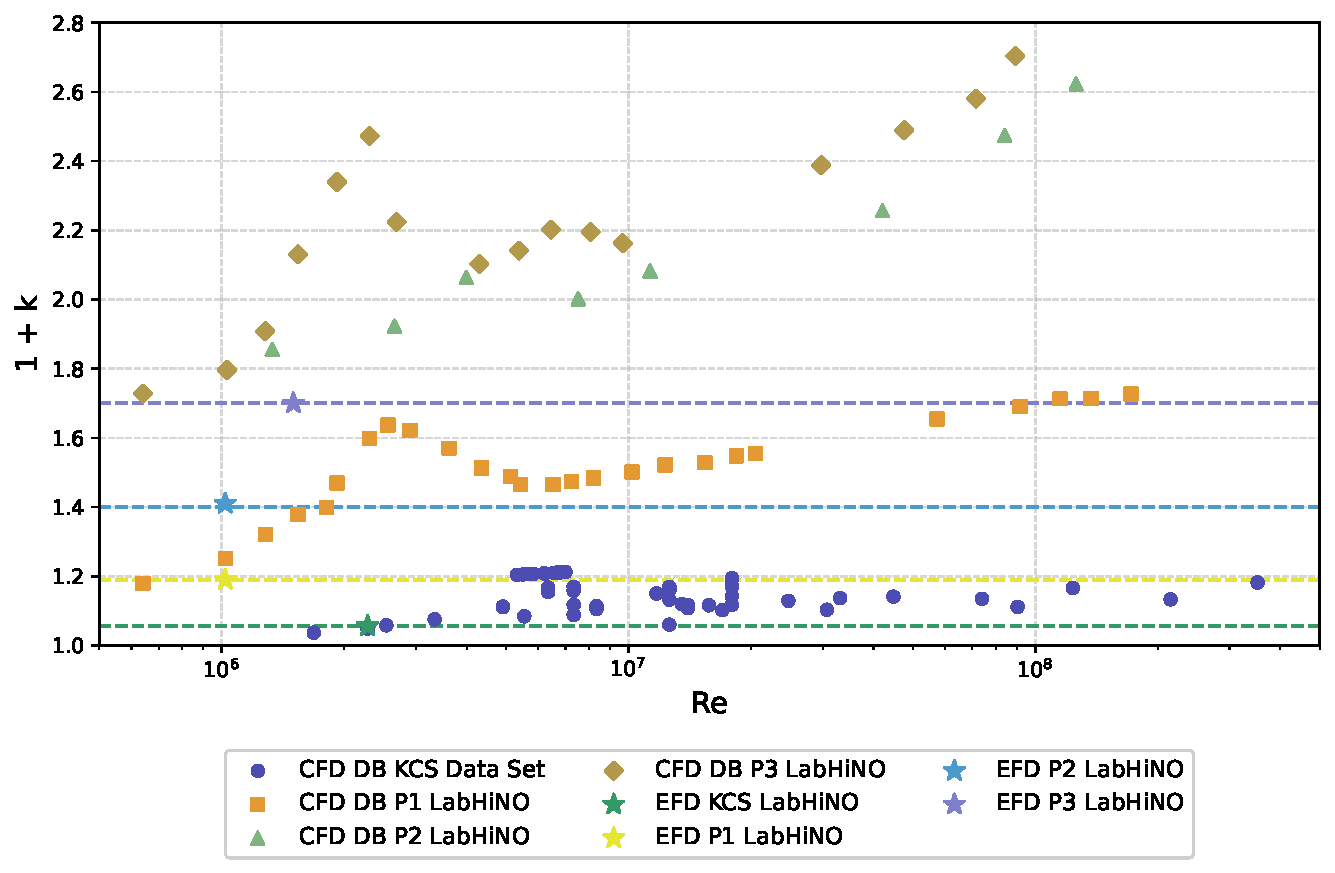
\includegraphics[width=\linewidth]{completo_log_kcs_lit_tpa_jpa_contessi.pdf}
\column{0.40\textwidth}
  \centering
  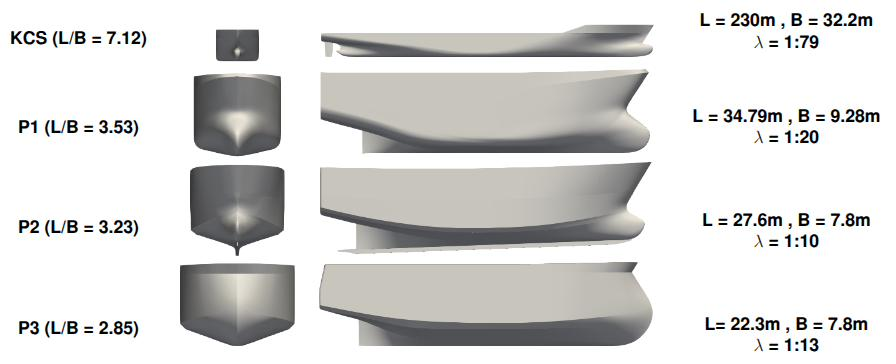
\includegraphics[width=\linewidth]{modelos_esbeltez.png}\\
  \fuente{Los cuatro cascos a igual eslora.}
  \vspace{0.5em}
  \begin{itemize}\small
    \item \Pu{} ($L/B=3.52$), \Pd{} (3.22) y \Pt{} (2.83): misma tendencia \alert{creciente y no asintótica}.
    \item Al bajar $L/B$: secciones más llenas y transición a popa más abrupta.
  \end{itemize}
\end{columns}
\mensaje{Rasgo estructural de los cascos con $L/B<4$, no una singularidad del \Pu.}
\note{1 min.}
\end{frame}

\begin{frame}{Mecanismo: la presión viscosa no escala}
\begin{columns}[c]
\column{0.55\textwidth}
  \centering
  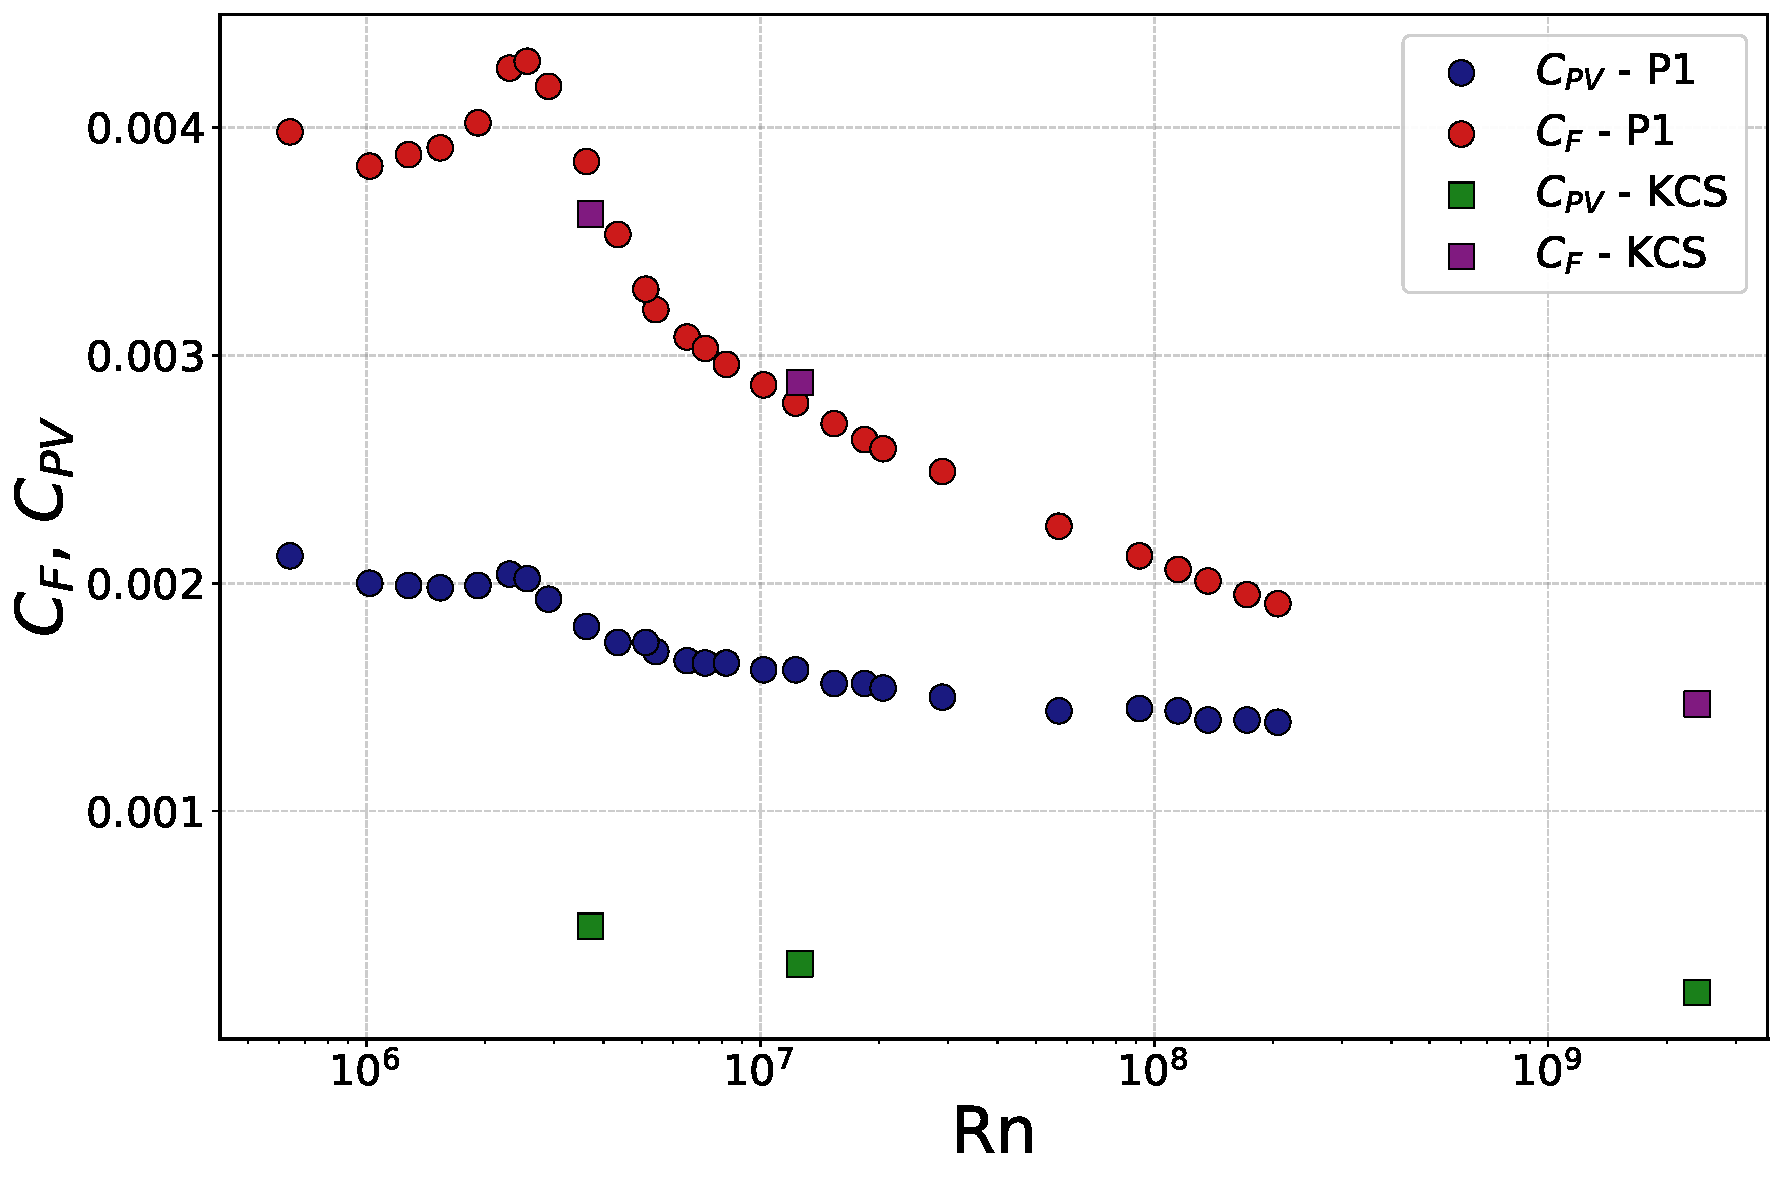
\includegraphics[width=\linewidth]{kcs_tpa_descomposicion.pdf}
\column{0.43\textwidth}
  \[\uk = \frac{C_V}{C_{F0}} = \underbrace{\frac{C_F}{C_{F0}}}_{\approx\,\text{cte}} + \alert{\frac{C_{PV}}{C_{F0}}}\]
  \begin{itemize}\small
    \item $C_F$ cae con $Re$ igual que $C_{F0}$.
    \item En el \Pu, $C_{PV}$ es \alert{alta y casi invariante} con la escala; en el \KCS{} es pequeña.
    \item El cociente $C_{PV}/C_{F0}$ crece: $\uk$ \alert{no puede estabilizarse}.
  \end{itemize}
\end{columns}
\mensaje{La descomposición que solo el CFD DB permite aísla la causa: la componente de presión viscosa.}
\note{1,5 min. Esta es la primera aparición del hilo conductor: el efecto de escala que no se corrige es de presión.}
\end{frame}

\begin{frame}{Origen físico: la popa llena}
\begin{columns}[c]
\column{0.58\textwidth}
  \centering
  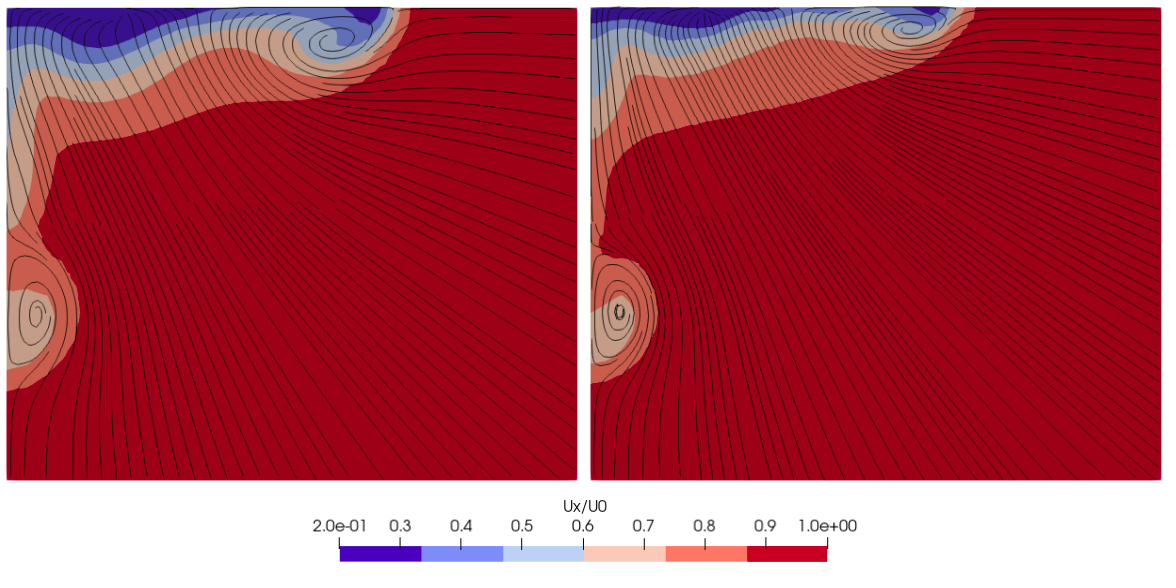
\includegraphics[width=0.86\linewidth]{U_x_U_0.png}\\
  \fuente{$U_x/U_0$ a $0.05\,L_{WL}$ aguas abajo del espejo. Izq.: 1:20 ($\log Re\approx6$). Der.: 1:1 ($\log Re\approx8$). $Fr=0.2$, T3.}
  \vspace{0.4em}
  \begin{itemize}\small
    \item Déficit de \alert{recuperación de presión} en el cuerpo de salida.
    \item Vórtices de \alert{quilla y pantoque} con extensión similar en ambas escalas: núcleo más concentrado, no debilitado.
  \end{itemize}
\column{0.40\textwidth}
  \centering
  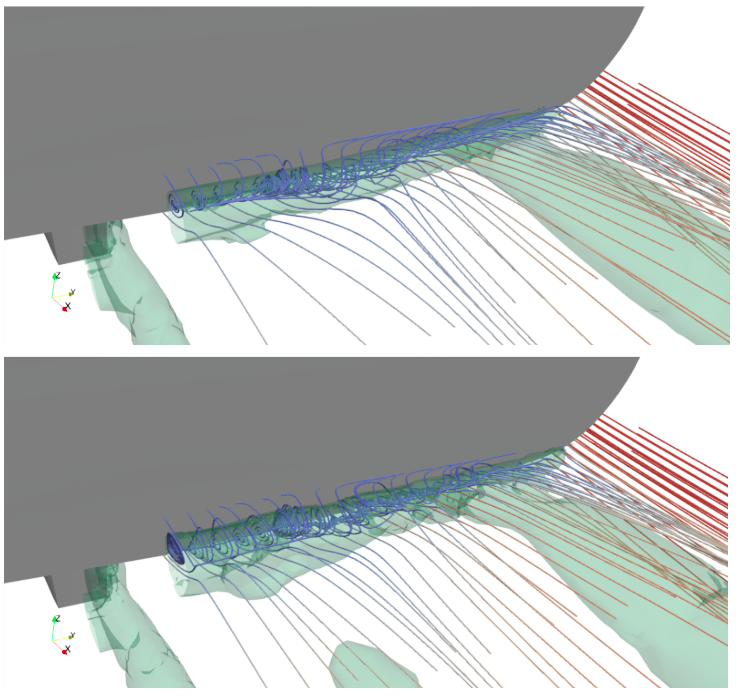
\includegraphics[width=0.88\linewidth]{vortex.png}\\
  \fuente{Criterio Q ($Q=10$). Arriba: 1:20. Abajo: 1:1.}
\end{columns}
\mensaje{Estructuras fijadas por la geometría $\Rightarrow$ $C_{PV}$ prácticamente invariante con la escala.}
\note{1,5 min.}
\end{frame}

\begin{frame}{Descartando causas alternativas (I)}
\begin{columns}[T]
\column{0.49\textwidth}
  \textbf{Proa bulbo}\\[2pt]
  \centering
  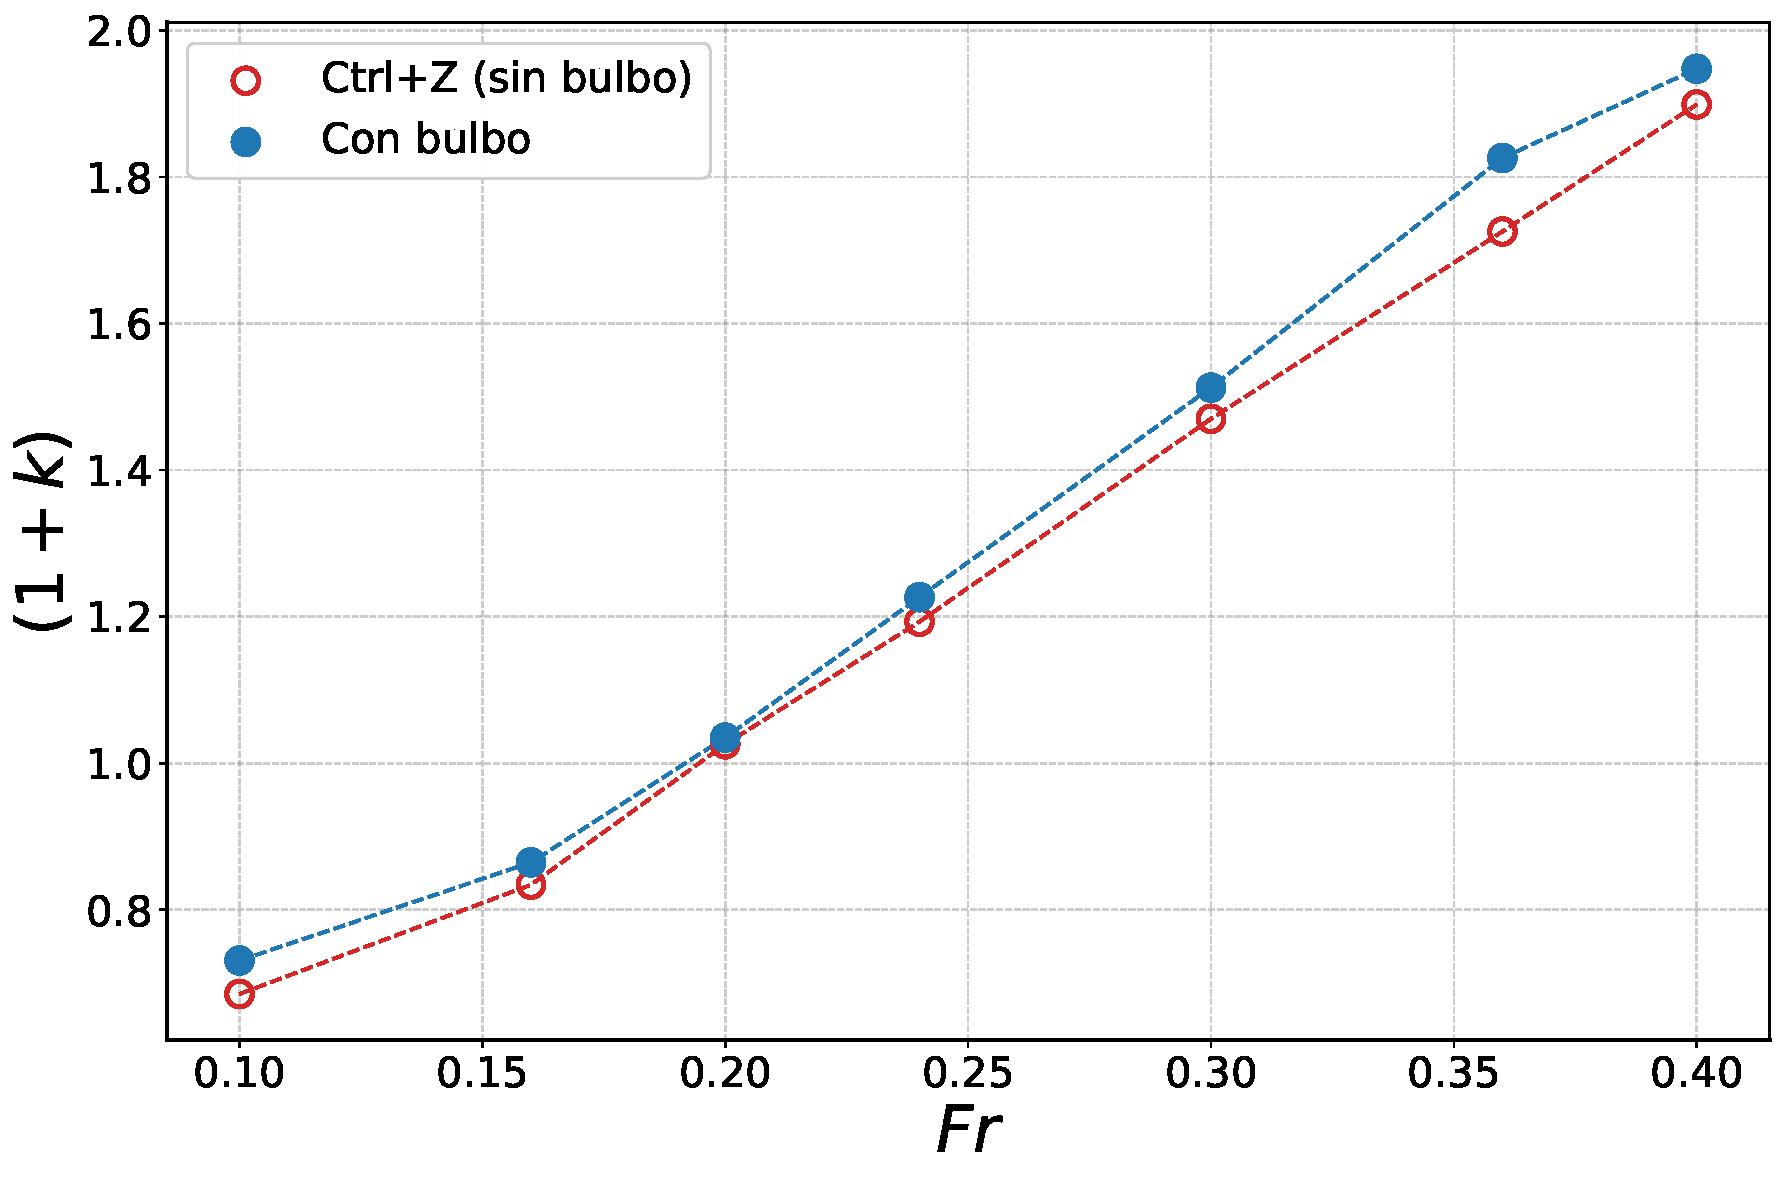
\includegraphics[height=3.4cm]{k-consinbulbo-195.pdf}
  \begin{itemize}\small
    \item El bulbo \alert{modifica} $\uk$ (efecto 3 veces mayor en carga ligera).
    \item Pero la curvatura de Prohaska y la falta de asíntota \alert{persisten sin bulbo}.
  \end{itemize}
\column{0.49\textwidth}
  \textbf{Popa espejo sumergida (método $2k$)}\\[2pt]
  \centering
  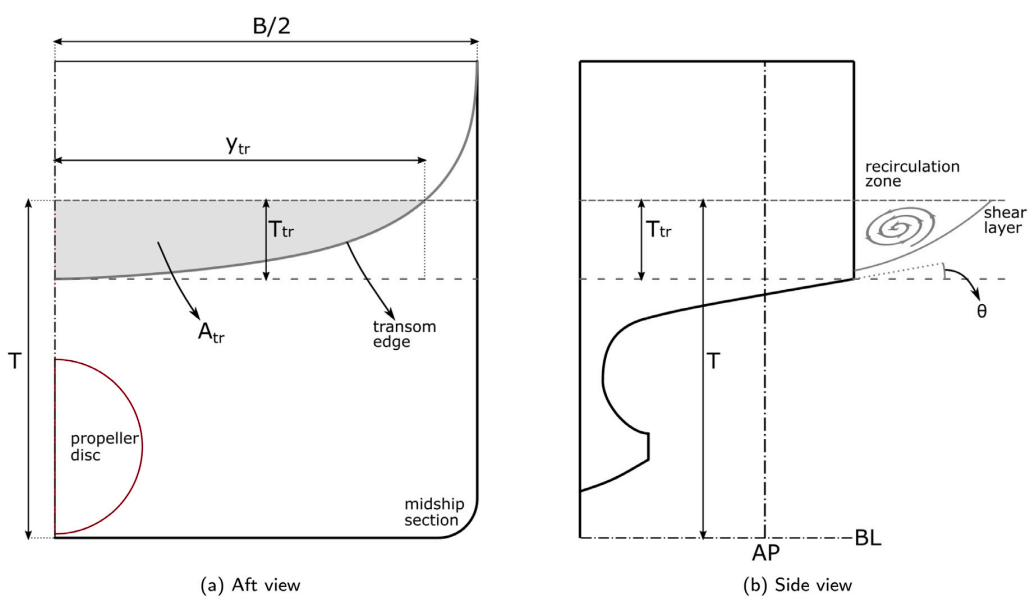
\includegraphics[height=3.4cm]{transom_scheme.png}
  \begin{itemize}\small
    \item Método de Korkmaz et al. (2022): $k_{tr} = 0.025$.
    \item Apenas \alert{$\approx$5\,\%} del efecto de escala total ($k_S-k_M = 0.522$).
  \end{itemize}
\end{columns}
\note{1,5 min. Las dos causas que la literatura señala como sospechosas habituales en Prohaska quedan descartadas como causa principal.}
\end{frame}

\begin{frame}{Descartando causas alternativas (II)}
\begin{columns}[T]
\column{0.49\textwidth}
  \textbf{Línea de fricción de referencia}\\[2pt]
  \centering
  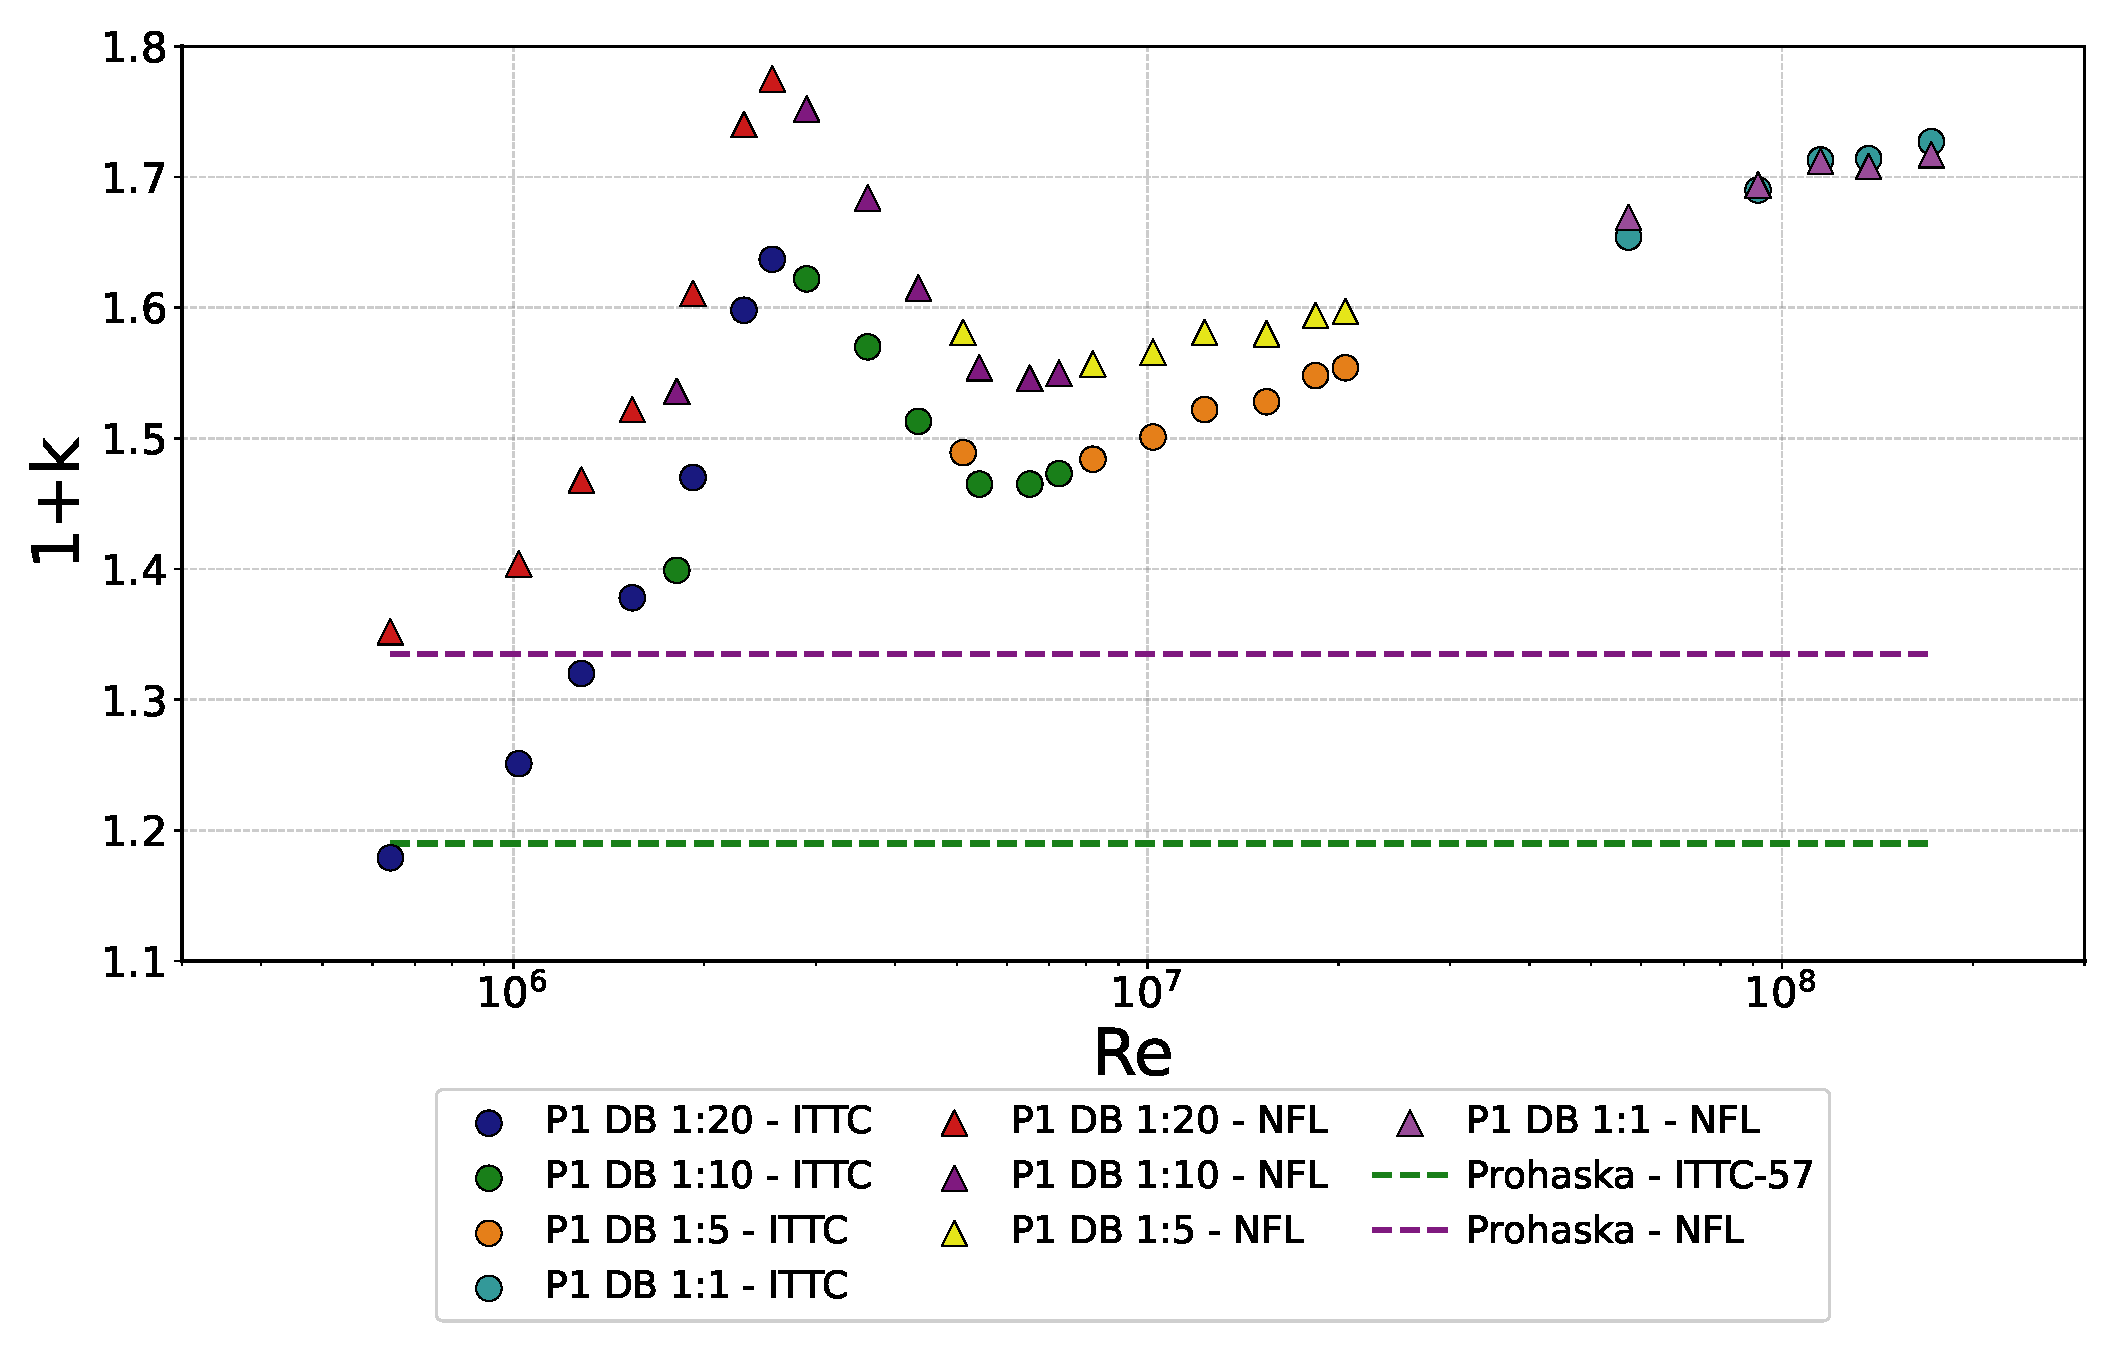
\includegraphics[height=3.3cm]{ittc-nfl.pdf}
  \begin{itemize}\small
    \item Con líneas numéricas (NFL), la variación baja de 40\,\% a \alert{$\sim$25\,\%}: se atenúa, \alert{no desaparece}.
    \item A escala buque, ambas líneas dan el mismo $\uk$.
  \end{itemize}
\column{0.49\textwidth}
  \textbf{Modelo de turbulencia}\\[2pt]
  \centering
  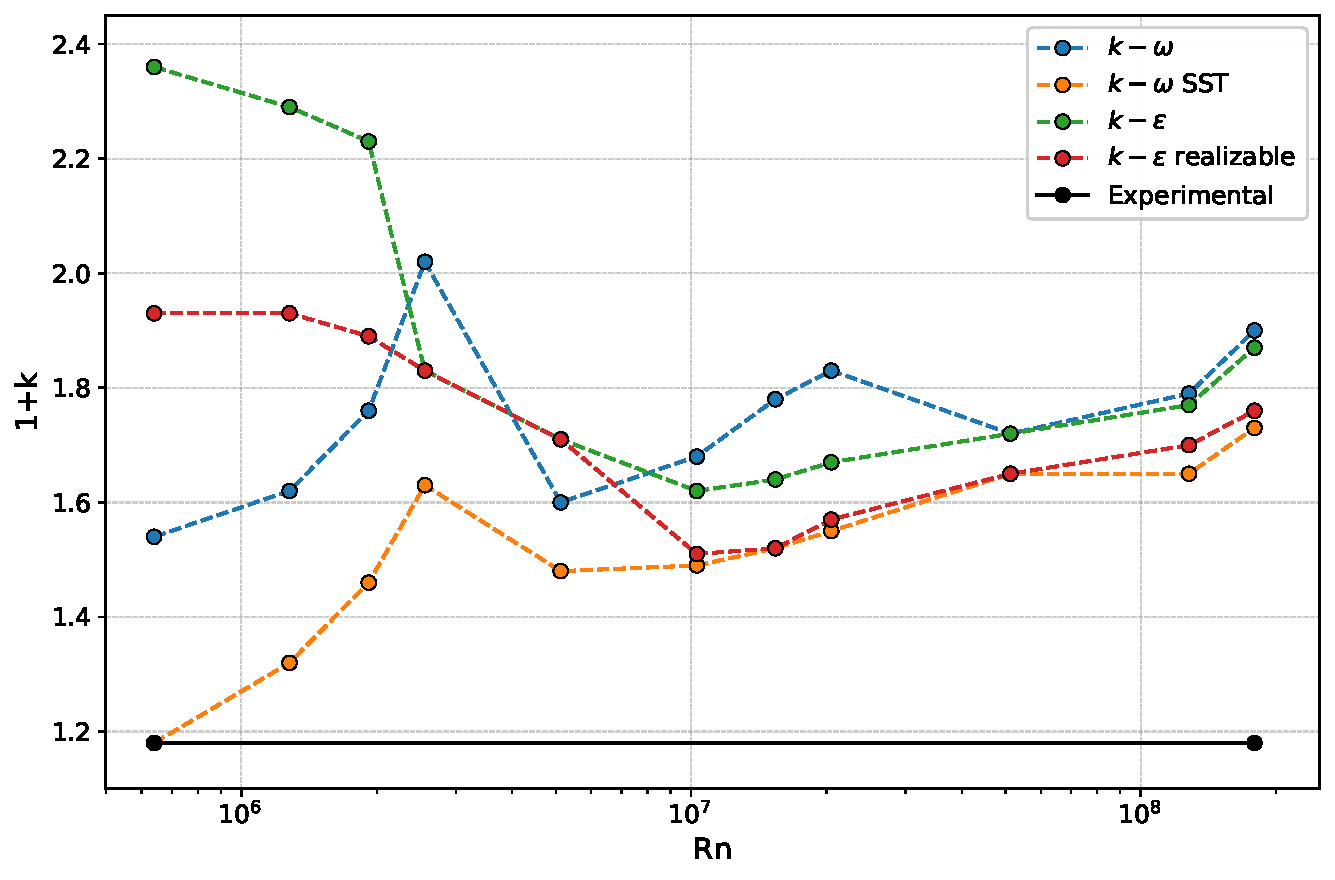
\includegraphics[height=3.3cm]{comparacion_k.pdf}
  \begin{itemize}\small
    \item Diferencias grandes a bajo $Re$; \alert{convergen} hacia escala buque.
    \item $k$–$\varepsilon$ sobrestima $\uk$ en régimen transicional; SST más alineado con EFD.
  \end{itemize}
\end{columns}
\mensaje{El efecto dominante es la evolución de $C_{PV}$, gobernada por la geometría de baja esbeltez.}
\note{1,5 min.}
\end{frame}

\begin{frame}{Correlaciones empíricas: navales frente a aerodinámicas}
\begin{columns}[T]
\column{0.49\textwidth}
  \centering
  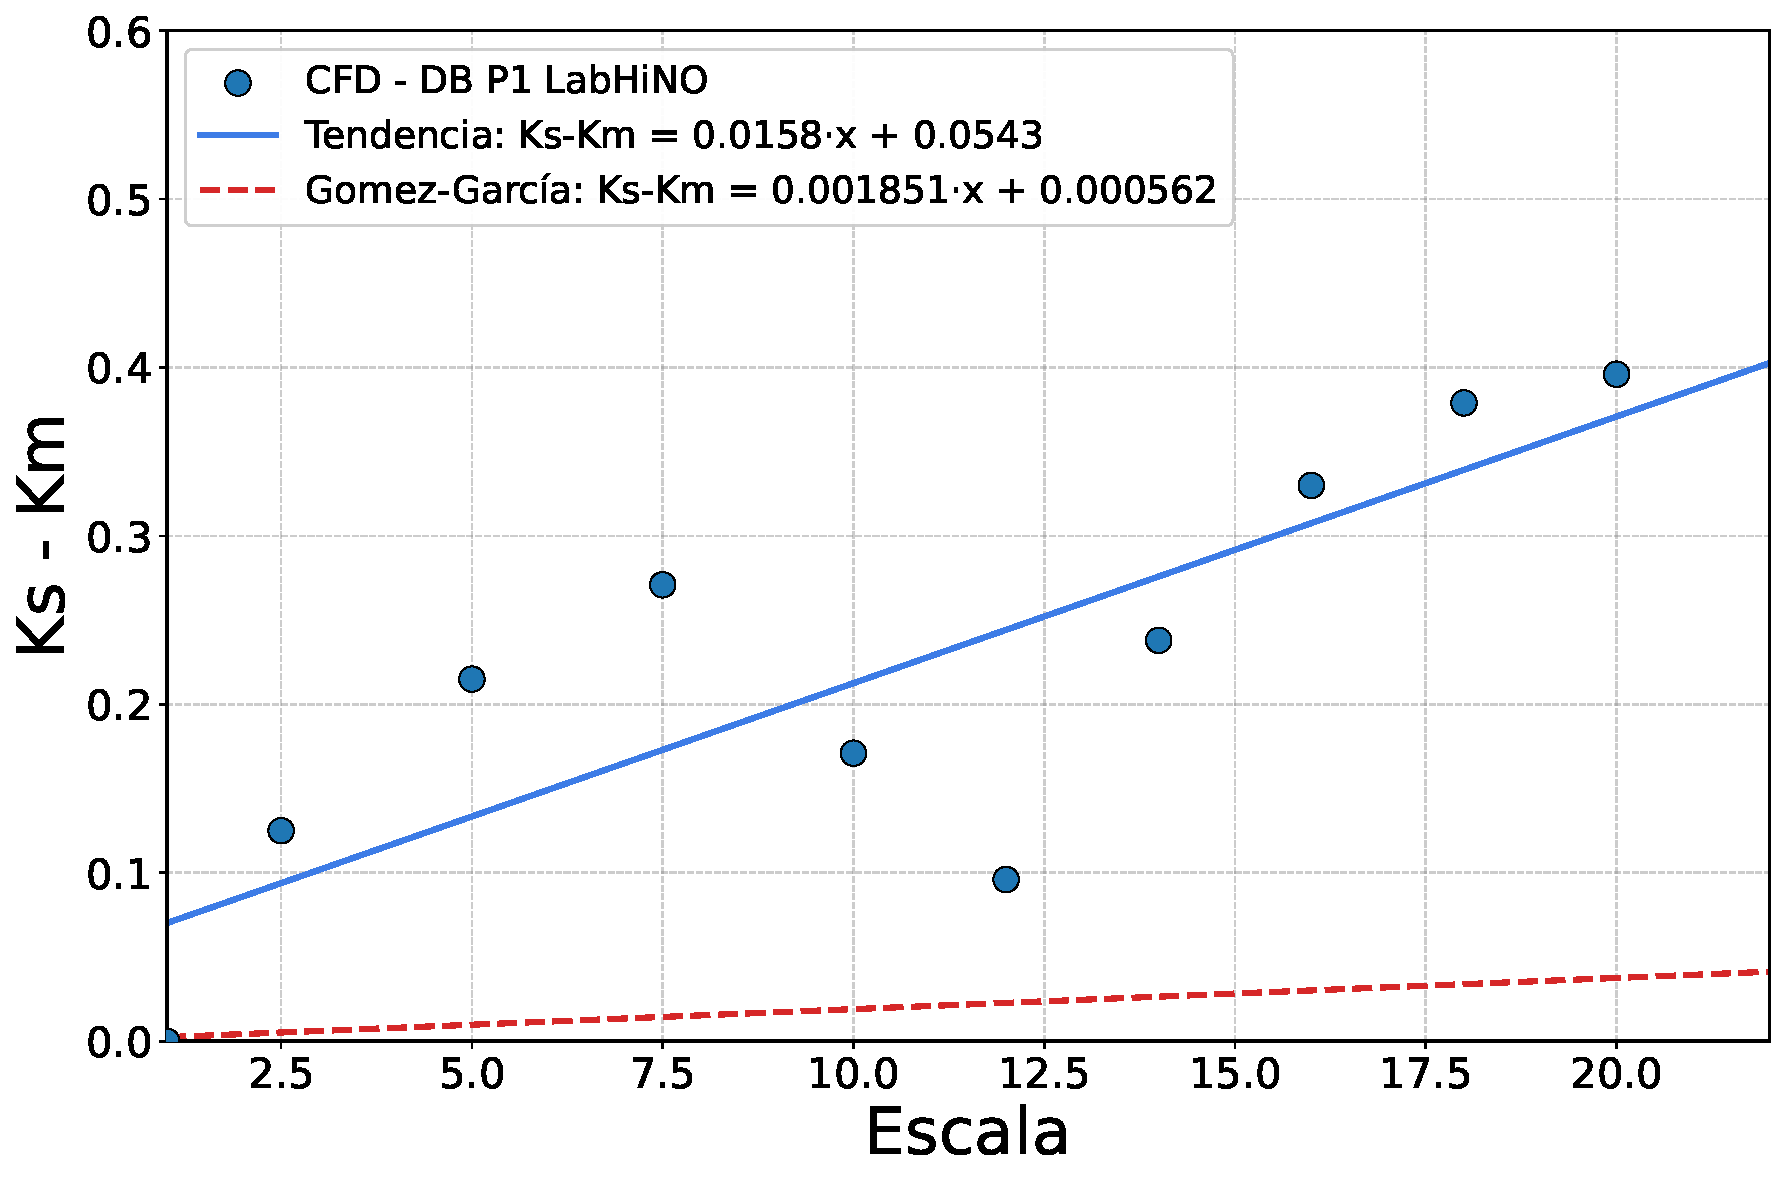
\includegraphics[width=0.72\linewidth]{gomez-garcia-nuestro.pdf}
  \begin{itemize}\small
    \item García-Gómez (2000), calibrada con $L/B = 6.98$–$9.07$: subestima el efecto de escala del \Pu{} en \alert{más de un orden de magnitud}.
  \end{itemize}
\column{0.49\textwidth}
  \centering
  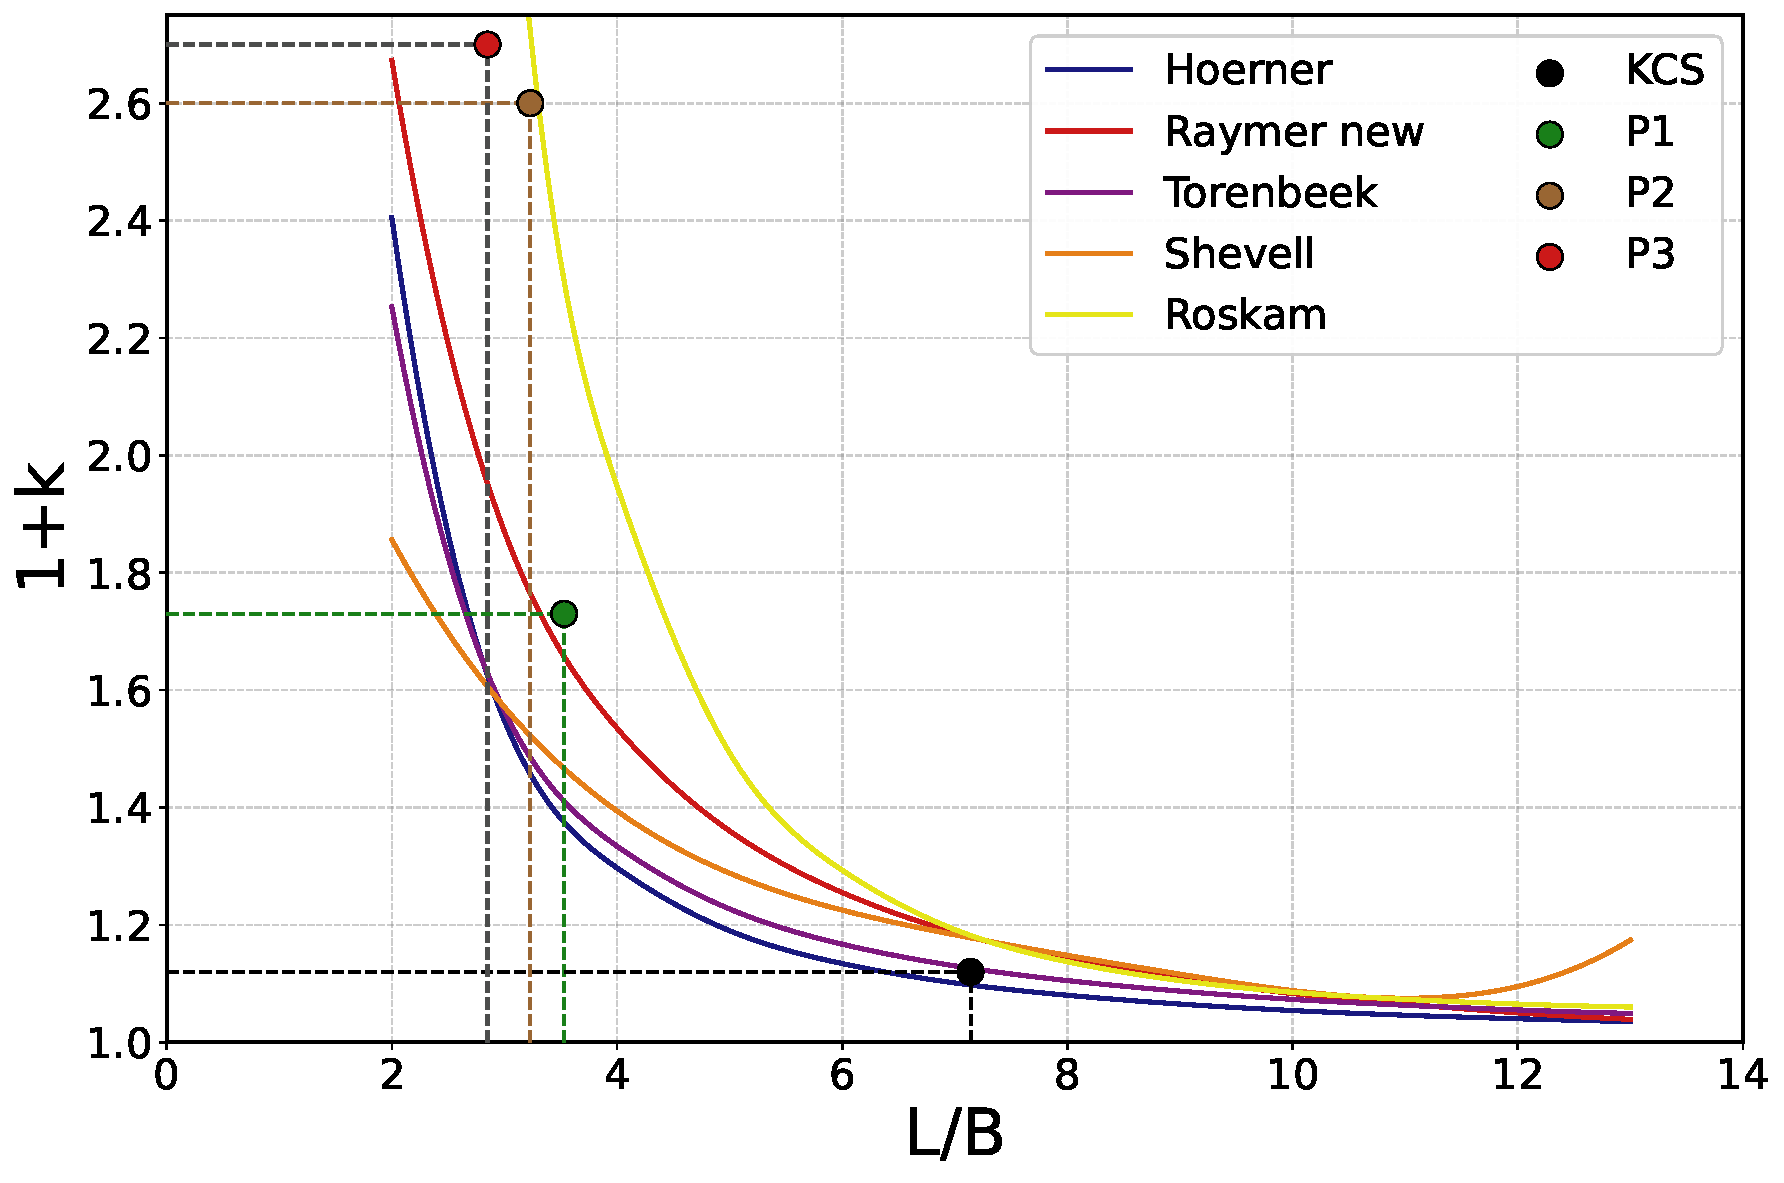
\includegraphics[width=0.72\linewidth]{aerodynamics2.pdf}
  \begin{itemize}\small
    \item Correlaciones de \alert{cuerpos de revolución} (Hoerner, Raymer, Torenbeek, Shevell, Roskam) ubican al \KCS{} y a los pesqueros de forma coherente con su $L/B$.
  \end{itemize}
\end{columns}
\mensaje{Abre la vía a una formulación $\uk = f(L/B)$ para cascos de baja esbeltez: doble $k$ sin CFD a escala buque.}
\note{1,5 min. Aporte propositivo, no solo diagnóstico.}
\end{frame}

\begin{frame}{Impacto sobre la potencia efectiva del \Pu}
\begin{columns}[c]
\column{0.50\textwidth}
  \small
  \textbf{M1} ITTC: $k_M = k_S$ (Prohaska EFD)\\
  \textbf{M2} Doble $k$: $k_M$ y $k_S$ de CFD DB\\
  \textbf{M3} $k=0$ (cota conservadora)
  \vspace{0.6em}

  \begin{tabular}{ccccc}
  \toprule
  $Fr$ & $V_S$ [kn] & \multicolumn{3}{c}{$P_{ES}$ [kW]} \\
  \cmidrule(lr){3-5}
  & & M1 & M2 & M3 \\
  \midrule
  0.26 & 9.16  & 151.5 & \alert{176.8} & 161.5 \\
  0.30 & 10.38 & 269.3 & \alert{305.5} & 283.3 \\
  \bottomrule
  \end{tabular}
\column{0.48\textwidth}
  \centering
  \begin{tikzpicture}
  \begin{axis}[
    ybar, width=6.6cm, height=4.6cm,
    bar width=13pt, enlarge x limits=0.45,
    ylabel={$\Delta P_{ES}$ vs. M1 [\%]}, ymin=0, ymax=20,
    symbolic x coords={Fr 0.26, Fr 0.30}, xtick=data,
    nodes near coords, nodes near coords style={font=\footnotesize},
    legend style={at={(0.5,1.03)},anchor=south,legend columns=2,font=\footnotesize,draw=none},
    tick label style={font=\footnotesize}, label style={font=\footnotesize},
    axis line style={gris}, ymajorgrids, grid style={gris!25}
  ]
  \addplot[fill=acento,draw=none] coordinates {(Fr 0.26,16.7) (Fr 0.30,13.4)};
  \addplot[fill=gris!60,draw=none] coordinates {(Fr 0.26,6.6) (Fr 0.30,5.2)};
  \legend{M2 doble $k$, M3 $k=0$}
  \end{axis}
  \end{tikzpicture}
\end{columns}
\mensaje{13–17\,\% de diferencia en potencia efectiva: \textbf{mayor que ignorar por completo el factor de forma} (5–7\,\%).}
\note{1,5 min. Remarcar la comparación con k=0: la discrepancia no viene del procedimiento sino de la magnitud del efecto de escala. Justifica validar con pruebas de mar.}
\end{frame}

\begin{frame}{Eje 1 en síntesis}
\begin{itemize}
  \item En pesqueros con $L/B<4$, $\uk$ \alert{crece sin asíntota} hasta escala buque: $\sim$40\,\% frente a $\sim$8\,\% en el \KCS.
  \item La causa es la \alert{presión viscosa de popa}, que no escala; bulbo, popa sumergida, línea de fricción y modelo de turbulencia no la explican.
  \item El supuesto $k_M = k_S$ introduce diferencias de \alert{13–17\,\%} en $P_E$.
  \item Las correlaciones navales fallan; las aerodinámicas en función de $L/B$ son una alternativa prometedora.
\end{itemize}
\note{30 s. Transición al Eje 2: “la misma pregunta, ahora en la hélice”.}
\end{frame}

% =====================================================================
\section{Eje 2: efectos de escala en hélices en aguas abiertas}
\note{Bloque objetivo: \textbf{12 min}.}
% =====================================================================

\begin{frame}{Hélices estudiadas y validación}
\begin{columns}[T]
\column{0.36\textwidth}
  \centering
  \begin{tabular}{cc}
  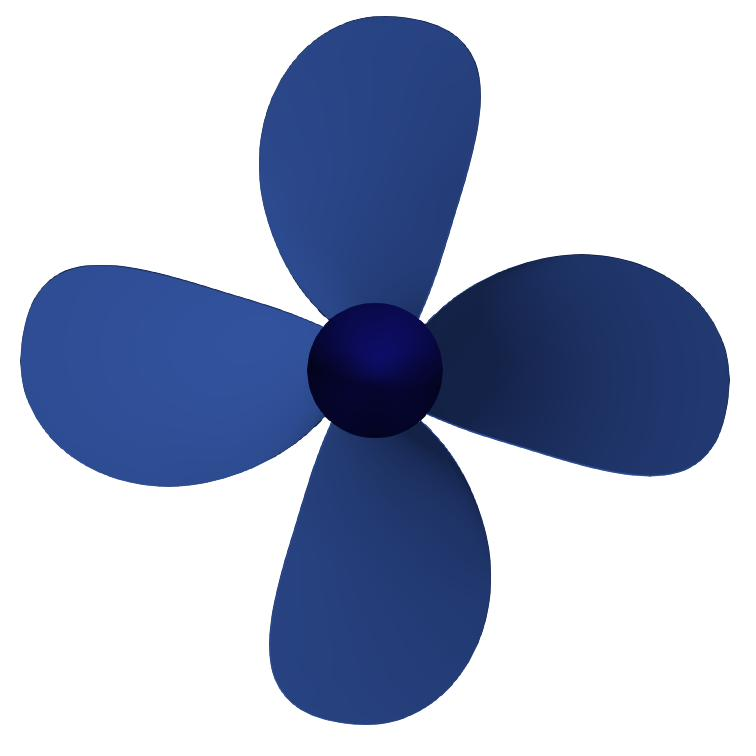
\includegraphics[height=2.2cm]{pala_wageningen.png} &
  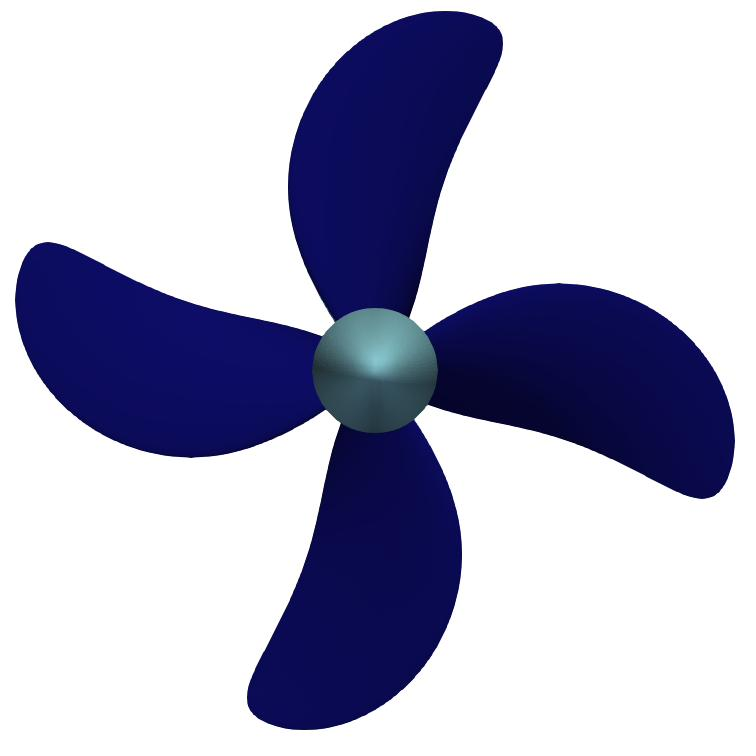
\includegraphics[height=2.2cm]{pala_p206.png}\\
  \small\Bfs & \small\Pdos
  \end{tabular}
  \begin{itemize}\footnotesize
    \item \Bfs: serie Wageningen, $P/D=0.81$, ensayos de archivo LabHiNO.
    \item \Pdos: $Z=4$, $A_E/A_0=0.431$, diseño no seriado; datos de túnel.
  \end{itemize}
\column{0.62\textwidth}
  \centering\small
  \Bfs, $J=0.5$, $Re_n = 3.2\times10^5$\\[3pt]
  \begin{tabular}{lccc}
  \toprule
  Fuente & $K_T$ & $10K_Q$ & $\eta_0$ \\
  \midrule
  LabHiNO (EFD) & 0.177 & 0.245 & 0.575 \\
  MARIN & 0.177 & 0.244 & 0.577 \\
  CFD SST & 0.186 {\scriptsize(+5.2\,\%)} & 0.270 {\scriptsize(+10.3\,\%)} & 0.548 \\
  CFD SST-LM & 0.190 {\scriptsize(+7.3\,\%)} & 0.264 {\scriptsize(+7.8\,\%)} & 0.573 \\
  \bottomrule
  \end{tabular}
  \vspace{0.5em}
  \begin{itemize}\footnotesize
    \item Diferencias de 5–7\,\% $>$ $U_{val}\approx1.7\,\%$: no validado en valor absoluto.
    \item Origen probable: geometría de serie \alert{sin planos} (bordes y punta) y régimen transicional.
    \item Uso: la \Bfs{} se emplea para \alert{diferencias entre escalas}, donde el sesgo geométrico se cancela en primer orden.
  \end{itemize}
\end{columns}
\note{1,5 min. Mejor decirlo nosotros antes de que lo pregunte el jurado: la limitación está cuantificada y el uso es coherente con ella.}
\end{frame}

\begin{frame}{\Bfs: barrido de diámetros $D = 0.14$–$8.0$\,m}
\begin{columns}[c]
\column{0.58\textwidth}
  \centering
  \begin{tikzpicture}
  \begin{axis}[
    width=8.4cm, height=5.6cm, xmode=log,
    xlabel={$Re_n = nD^2/\nu$}, ylabel={$K_T$},
    ymin=0.184, ymax=0.197, yticklabel style={/pgf/number format/.cd,fixed,precision=3},
    legend style={at={(0.03,0.97)},anchor=north west,font=\footnotesize,draw=none,fill=white,fill opacity=0.85,text opacity=1}, ytick={0.185,0.188,0.191,0.194,0.197},
    tick label style={font=\footnotesize}, label style={font=\footnotesize},
    axis line style={gris}, grid=major, grid style={gris!25}
  ]
  \addplot[navy,thick,mark=*,mark size=1.8pt] coordinates {
    (3.2e5,0.186) (2.4e6,0.188) (9.6e6,0.191) (1.92e7,0.193) (3.84e7,0.194) (7.68e7,0.195)};
  \addplot[acento,thick,dashed,mark=diamond*,mark size=2.2pt] coordinates {
    (3.2e5,0.1860) (2.4e6,0.1864) (9.6e6,0.1868) (1.92e7,0.1870) (3.84e7,0.1872) (7.68e7,0.1873)};
  \legend{CFD SST (directo), ITTC-78 desde $D=0.14$\,m}
  \end{axis}
  \end{tikzpicture}\\
  \fuente{Datos de la tabla del barrido ($J=0.5$). ITTC-78 recalculado con $c_{0.75R}/D=0.309$, $t/c=0.033$, superficie lisa.}
\column{0.40\textwidth}
  \begin{itemize}\small
    \item $J = 0.5$, SST, malla escalada geométricamente.
    \item $Re_n$: $3.2\times10^5 \rightarrow 7.7\times10^7$.
  \end{itemize}
  \vspace{0.3em}
  \begin{dato}
  \small
  $\Delta K_T = \alert{+4.7\,\%}$\\
  $\Delta K_Q = -4.1\,\%$\\
  $\Delta\eta_0 = \alert{+9.1\,\%}$
  \end{dato}
  \begin{itemize}\small
    \item El empuje crece por \alert{presión} ($K_{Tp}$), no por fricción.
  \end{itemize}
\end{columns}
\note{1 min.}
\end{frame}

\begin{frame}{El aumento de empuje es de presión}
\centering
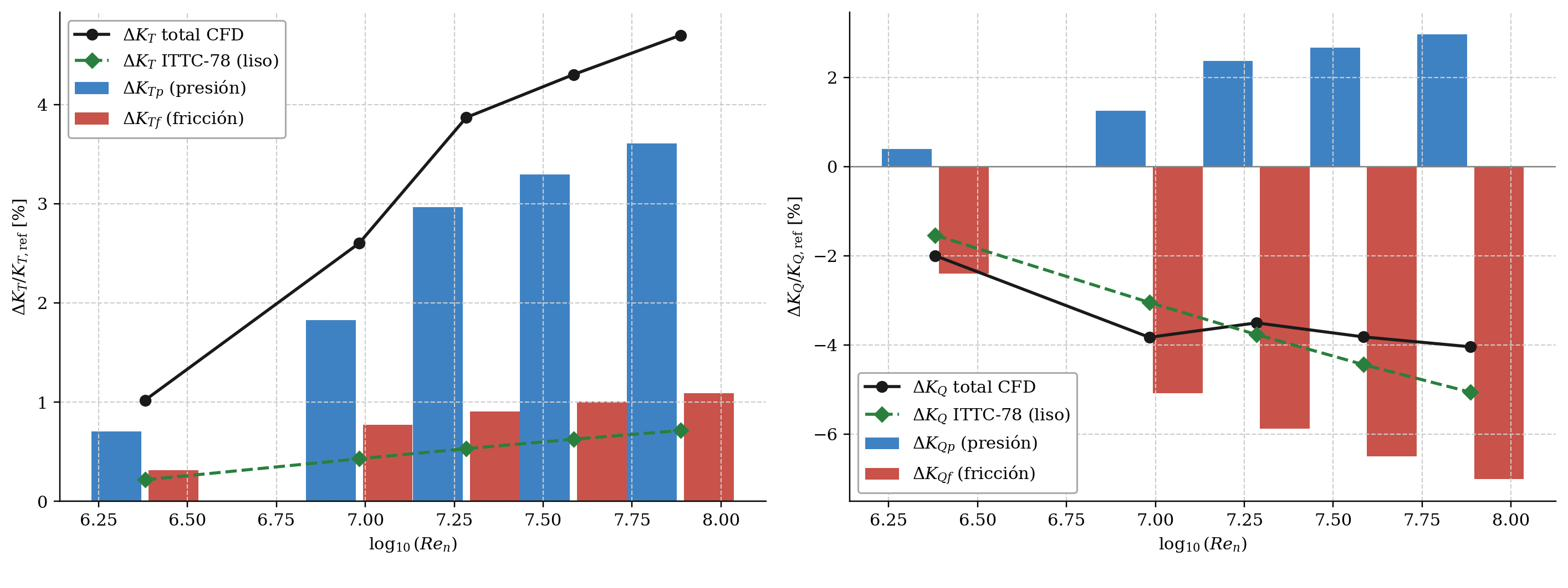
\includegraphics[width=0.86\linewidth]{fig2_delta_descomp.png}
\vspace{0.3em}
\begin{columns}[T]
\column{0.48\textwidth}
  \small\textbf{Empuje:} $\Delta K_{Tp}/\Delta K_T \approx$ \alert{76–77\,\%} (para $D\ge1$\,m). Solo un cuarto proviene de la reducción de fricción.
\column{0.48\textwidth}
  \small\textbf{Par:} la reducción está dominada por la fricción; $\Delta K_{Qp}$ es pequeño y \alert{positivo}.
\end{columns}
\mensaje{El efecto de escala completamente turbulento sobre el empuje es mayoritariamente de \textbf{presión}.}
\note{1,5 min. Segunda aparición del hilo conductor.}
\end{frame}

\begin{frame}{Dónde ocurre: lado de succión, mitad externa de la pala}
\begin{columns}[c]
\column{0.50\textwidth}
  \centering
  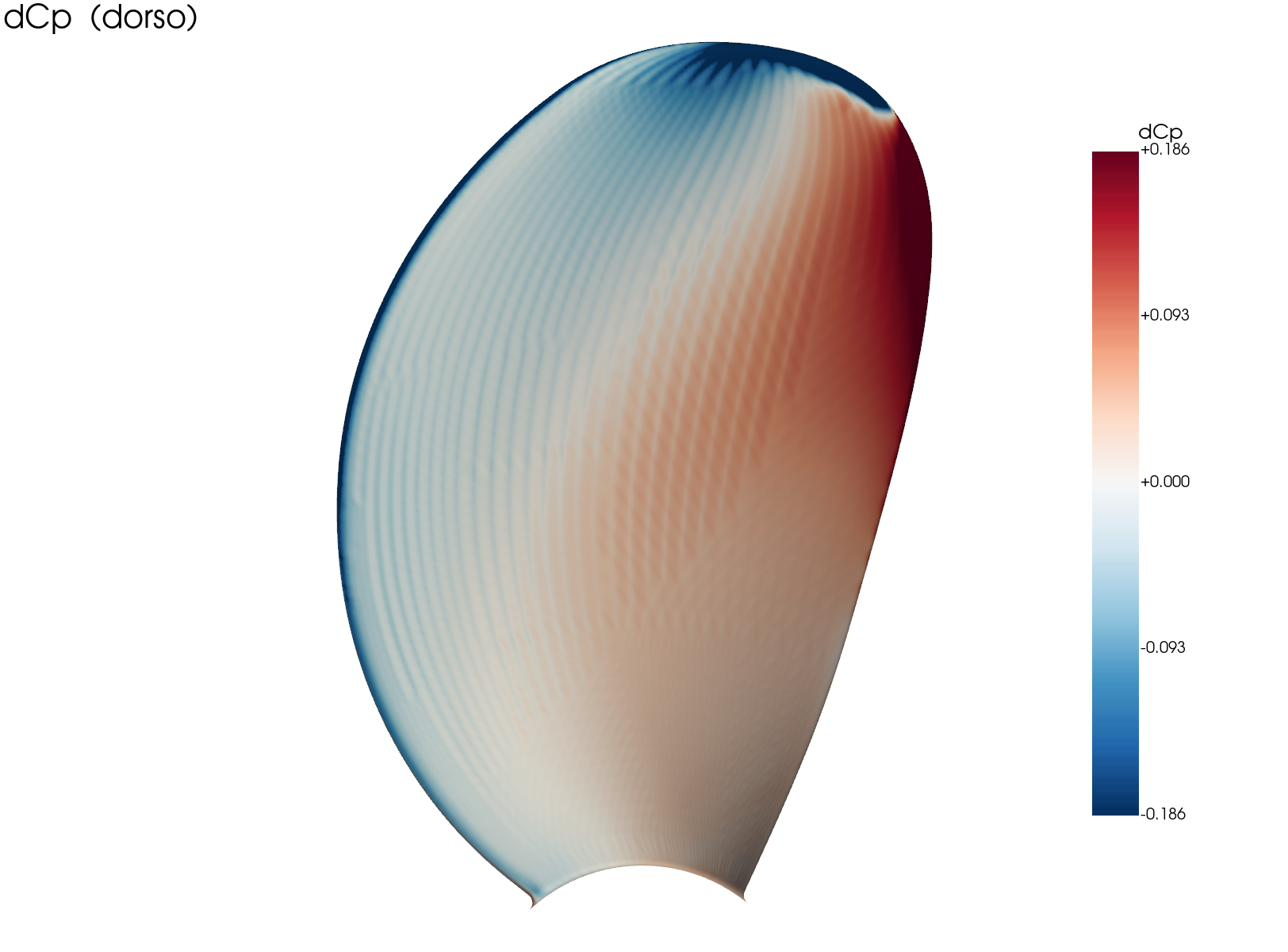
\includegraphics[width=0.49\linewidth]{delta_cp_dorso.png}\hfill
  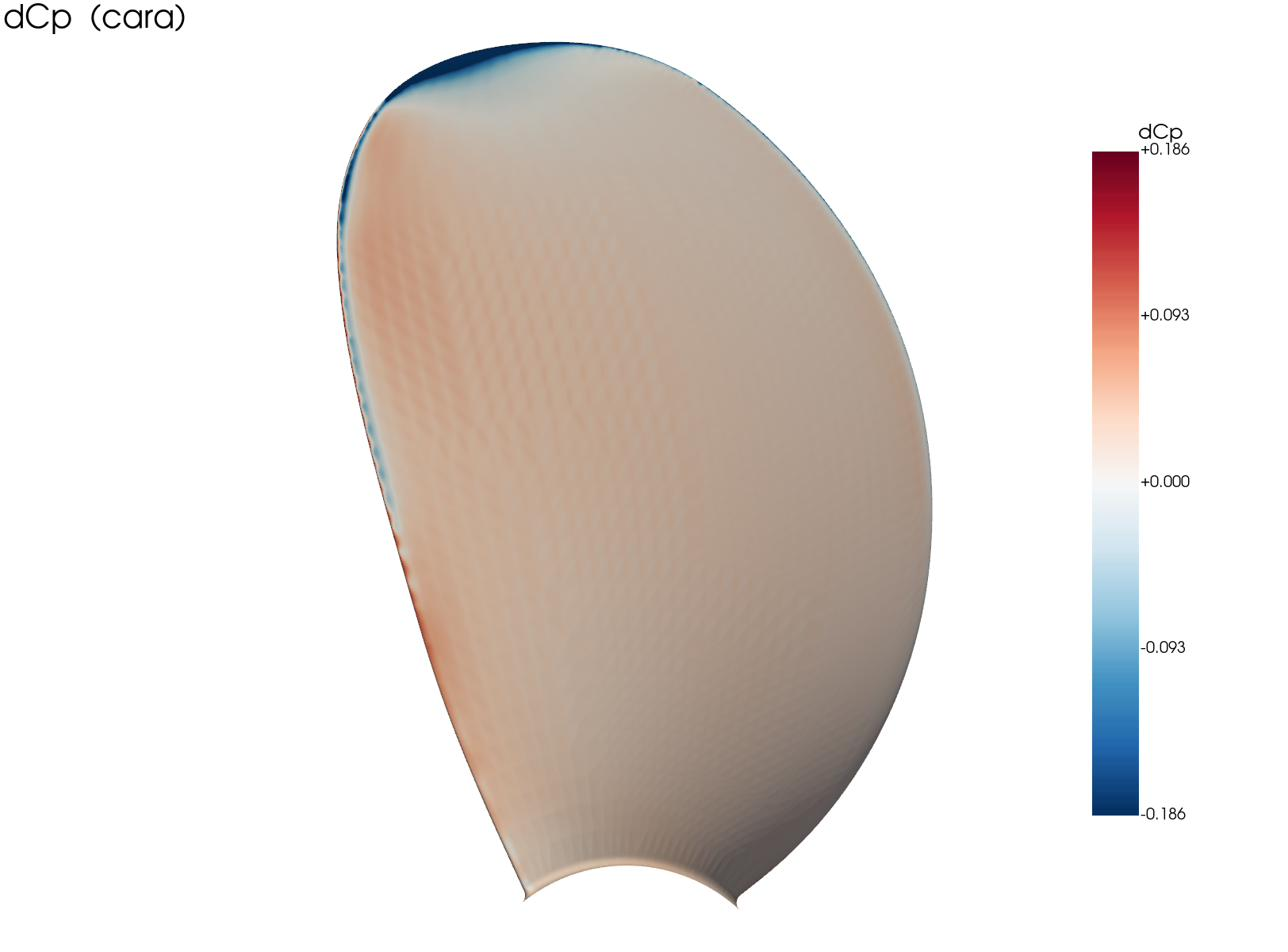
\includegraphics[width=0.49\linewidth]{delta_cp_cara.png}\\
  \fuente{$\Delta C_p$ entre $Re_n=10^4$ y $\approx2.5\times10^6$. Izq.: dorso. Der.: cara.}
\column{0.48\textwidth}
  \centering
  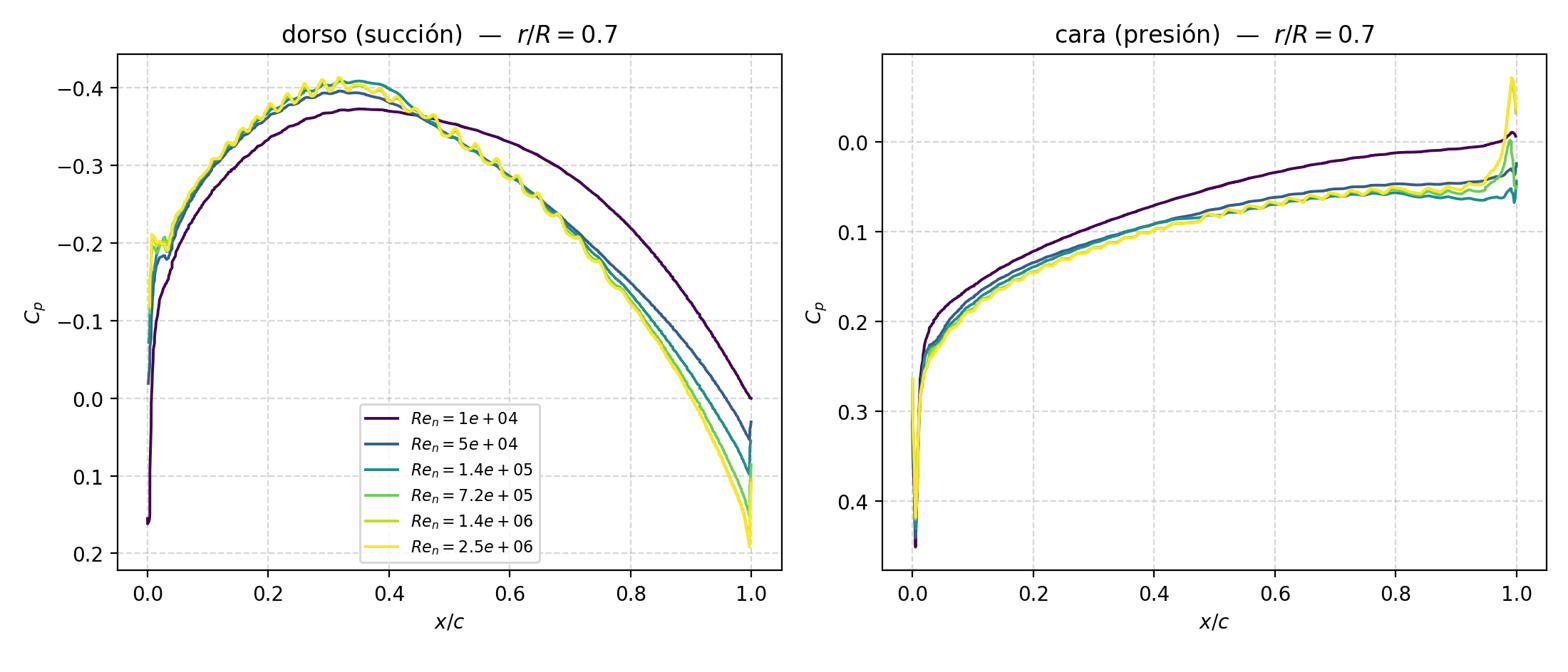
\includegraphics[width=\linewidth]{cp_section_r07.png}\\
  \fuente{$C_p$ en $r/R=0.7$ para las escalas del barrido.}
\end{columns}
\vspace{0.5em}
\begin{itemize}\small
  \item La redistribución se concentra en el \alert{dorso} y se intensifica hacia la punta.
  \item El \alert{pico de succión} del borde de ataque se profundiza con $Re$; la cara es poco sensible.
\end{itemize}
\note{1 min.}
\end{frame}

\begin{frame}{Consecuencia: el ITTC-78 subestima la ganancia a escala buque}
\begin{columns}[c]
\column{0.56\textwidth}
  \centering
  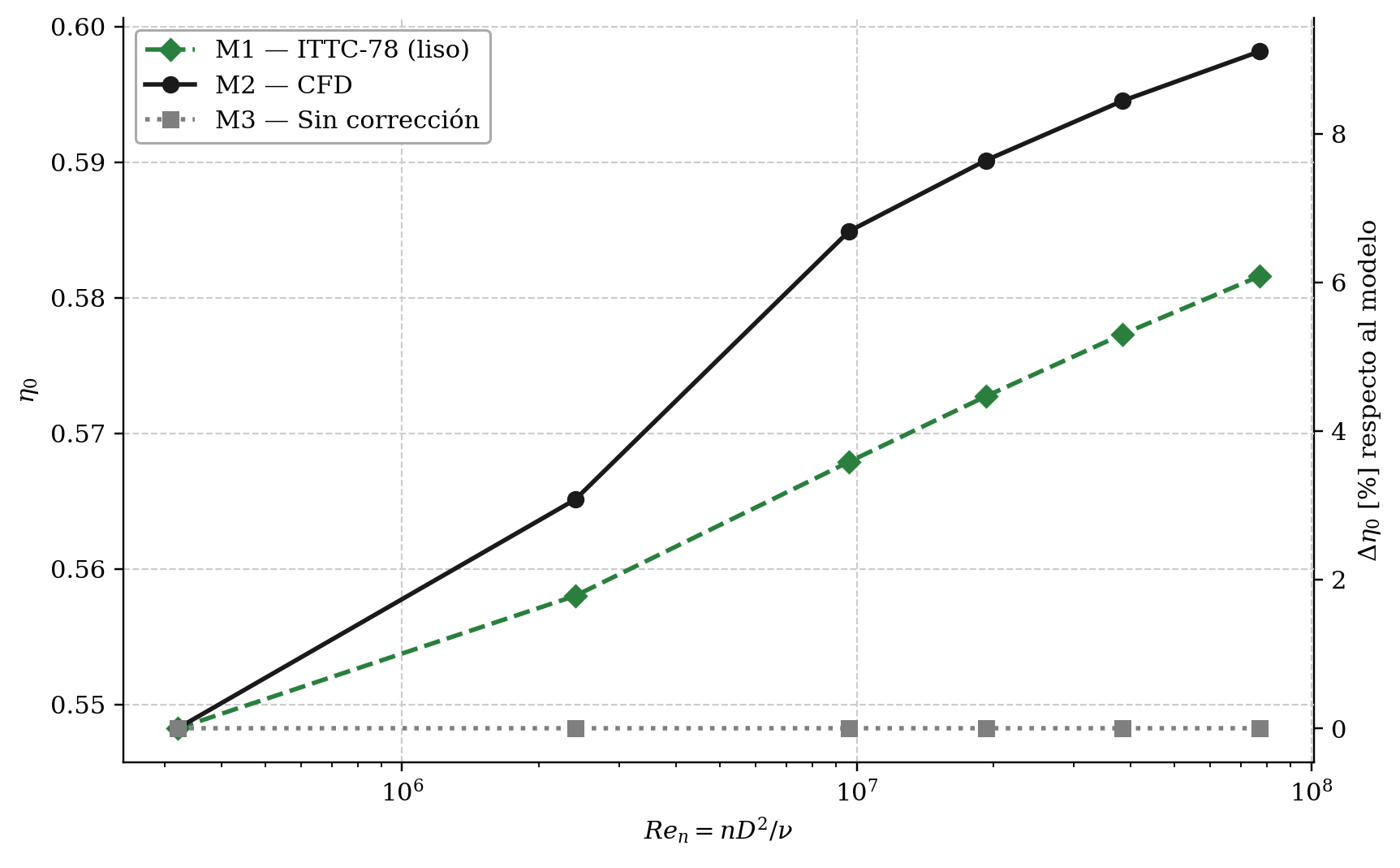
\includegraphics[width=\linewidth]{fig2b_eficiencia.png}\\
  \fuente{M1: ITTC-78 · M2: CFD SST · M3: sin corrección. $J=0.5$.}
\column{0.42\textwidth}
  \centering\small
  $D = 8.0$\,m (referencia $D = 0.14$\,m)\\[3pt]
  \begin{tabular}{lccc}
  \toprule
  & ITTC-78 & CFD & Dif. \\
  \midrule
  $K_T$ & 0.188 & 0.195 & \alert{+4.0\,\%} \\
  $10K_Q$ & 0.257 & 0.259 & +1.1\,\% \\
  $\eta_0$ & 0.582 & 0.598 & +2.8\,\% \\
  \bottomrule
  \end{tabular}
  \vspace{0.5em}
  \begin{itemize}\footnotesize
    \item Ganancia de $\eta_0$: CFD \alert{+9.1\,\%} vs. ITTC-78 \alert{+6.1\,\%}: brecha de 3.0 puntos.
    \item El ITTC-78 recupera $\sim$\alert{1/6} del aumento de empuje.
  \end{itemize}
\end{columns}
\note{1,5 min. Sesgo conservador pero no despreciable para dimensionar la instalación propulsora.}
\end{frame}

\begin{frame}{\Pdos: la joroba transicional}
\centering
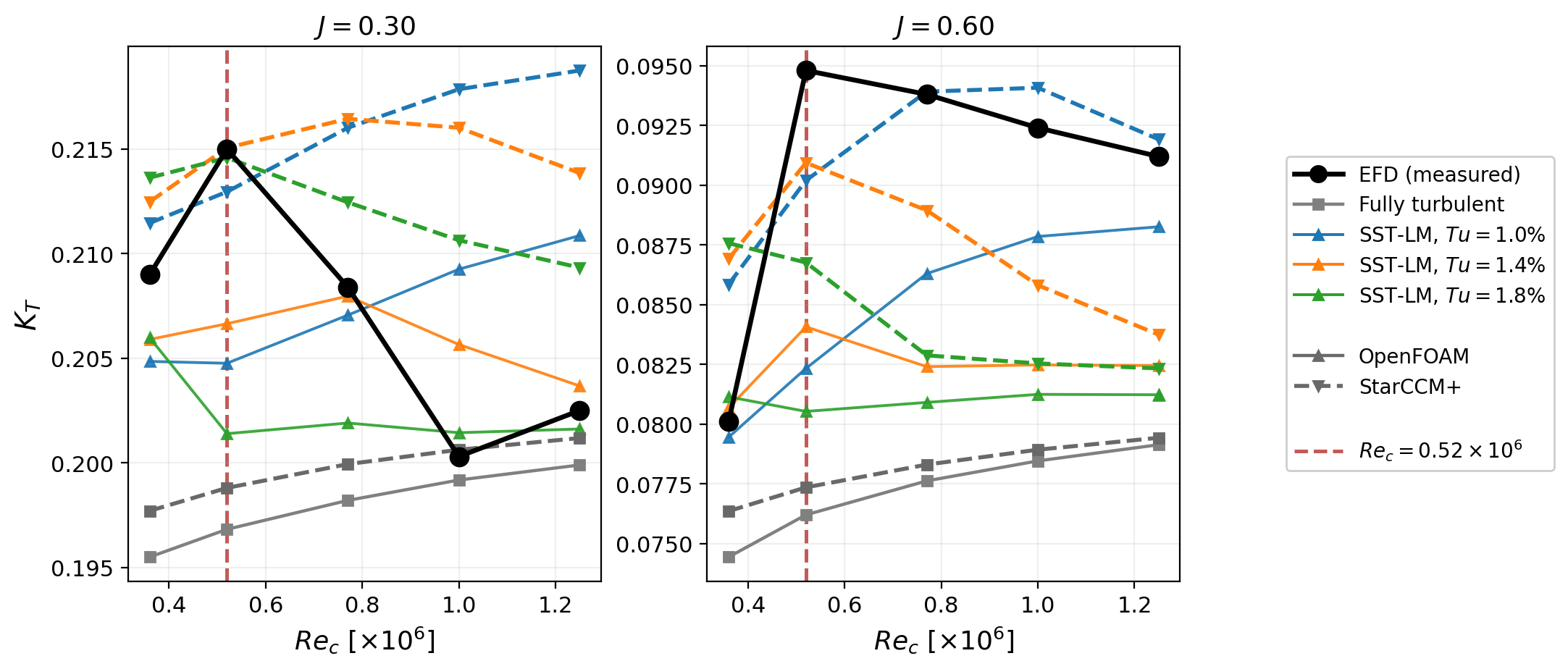
\includegraphics[width=0.84\linewidth]{fig_chichon_en.png}
\begin{columns}[T]
\column{0.48\textwidth}
  \begin{itemize}\footnotesize
    \item $Re_c = 0.36$–$1.25\times10^6$; máximo en $Re_c\approx0.52\times10^6$.
    \item Amplitud: \alert{7.1\,\%} ($J=0.30$) a \alert{16.3\,\%} ($J=0.60$).
  \end{itemize}
\column{0.48\textwidth}
  \begin{itemize}\footnotesize
    \item SST completamente turbulento: \alert{no la reproduce}.
    \item SST-LM (OpenFOAM y StarCCM+): la captura parcialmente; \alert{ningún $Tu$ único} ajusta todo el rango.
  \end{itemize}
\end{columns}
\note{1,5 min. Tu no es una propiedad transferible: el mejor valor cambia con J y con el solver.}
\end{frame}

\begin{frame}{La joroba también es de presión}
\centering
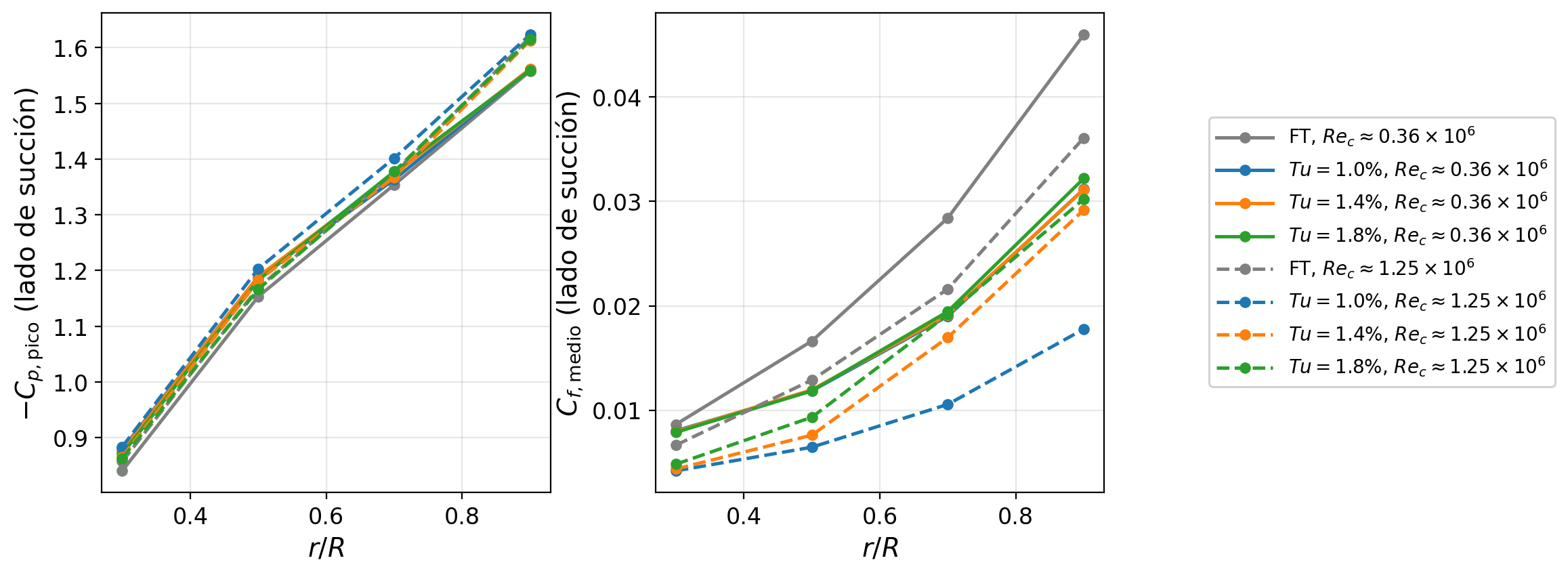
\includegraphics[width=0.86\linewidth]{cpn_cf_vs_rR_succion_es.png}
\begin{itemize}\small
  \item Desplazamiento de la curva completamente turbulenta hacia el SST-LM: \alert{$\sim$90\,\% de presión}.
  \item El par \alert{aumenta} levemente con SST-LM; una reducción puramente friccional lo disminuiría.
  \item La transición se ve nítida en $C_f$ (frente dependiente de $Tu$; cizalla más radial: 0.19 $\rightarrow$ 0.40–0.43), pero el pico de succión cambia $<3.1\,\%$: es una \alert{redistribución de carga} en envergadura.
\end{itemize}
\note{1,5 min.}
\end{frame}

\begin{frame}{Extrapolar desde el régimen transicional}
\centering
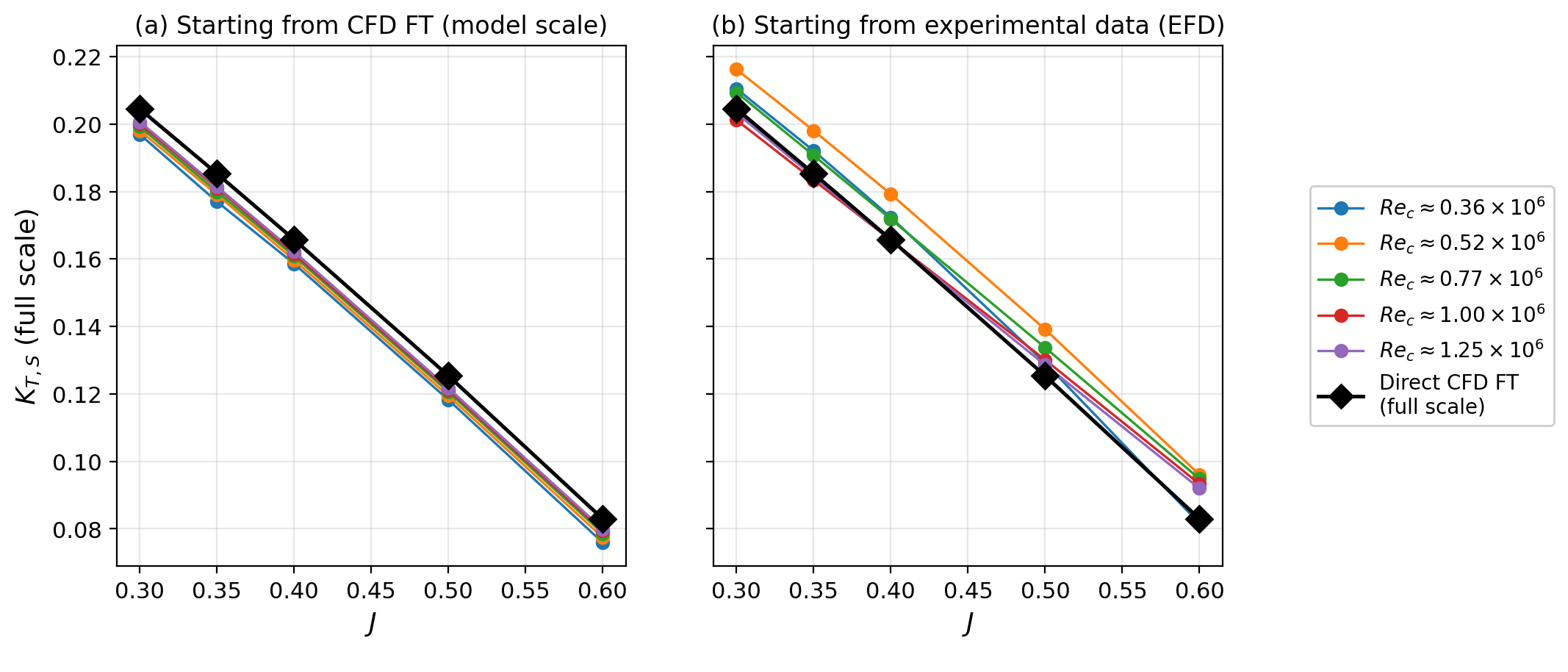
\includegraphics[width=0.70\linewidth]{fig_ittc78_vs_cfd_en.png}\\
\fuente{ITTC-78 aplicado a cada punto de escala modelo, frente al CFD resuelto a escala buque ($D=6$\,m).}
\begin{columns}[T]
\column{0.48\textwidth}
  \begin{itemize}\footnotesize
    \item \textbf{Base completamente turbulenta:} sesgo sistemático de \alert{$-2$ a $-10\,\%$} en $K_{TS}$, creciente al descargar.
  \end{itemize}
\column{0.48\textwidth}
  \begin{itemize}\footnotesize
    \item \textbf{Base EFD:} el punto en la joroba da \alert{+5.5 a +14.5\,\%}; dispersión de hasta \alert{17.7 puntos} ($J=0.60$).
  \end{itemize}
\end{columns}
\mensaje{El resultado depende de \textbf{a qué velocidad de giro} se hizo el único ensayo de túnel disponible.}
\note{1,5 min. Riesgo práctico: sin saber si el Re\_c del ensayo cae en la joroba, el error puede duplicarse o triplicarse.}
\end{frame}

\begin{frame}{Fracción de presión del efecto de escala}
\begin{columns}[c]
\column{0.52\textwidth}
  \centering
  \begin{tikzpicture}
  \begin{axis}[
    xbar, width=7.2cm, height=4.4cm, bar width=12pt,
    xmin=0, xmax=1.3, xtick={0,0.2,0.4,0.6,0.8,1.0}, xlabel={$f_p = \Delta K_{Tp}/\Delta K_T$},
    symbolic y coords={B4-60, P1727, P206}, ytick=data,
    enlarge y limits=0.3,
    nodes near coords, nodes near coords align={horizontal},
    point meta=explicit symbolic,
    every node near coord/.append style={font=\footnotesize,anchor=west},
    tick label style={font=\footnotesize}, label style={font=\footnotesize},
    axis line style={gris}, xmajorgrids, grid style={gris!25}
  ]
  \addplot[fill=acento,draw=none] coordinates {
    (0.765,B4-60) [0.70–0.77]
    (0.88,P1727) [$\approx$0.88]
    (0.91,P206) [0.90–0.92]};
  \end{axis}
  \end{tikzpicture}\\
  \fuente{\textit{P1727}: a partir de Gallotti y Gaggero (2026).}
\column{0.46\textwidth}
  \begin{itemize}\small
    \item \Pdos{} ($A_E/A_0 = 0.431$) y \textit{P1727} (0.444), geométricamente afines, coinciden en la banda alta.
    \item Hipótesis: $f_p$ gobernada por el \alert{área expandida reducida}.
    \item En la \Pdos, una corrección friccional explica a lo sumo el \alert{8–10\,\%} del efecto real.
  \end{itemize}
\end{columns}
\mensaje{La generalización con la geometría de la pala requiere un mapeo sistemático: el eje propulsivo queda más abierto que el de resistencia.}
\note{1 min.}
\end{frame}

\begin{frame}{Eje 2 en síntesis}
\begin{itemize}
  \item Efecto de escala completamente turbulento (\Bfs): el empuje crece por \alert{presión} (76–77\,\%); el ITTC-78 subestima la ganancia de $\eta_0$ en 3 puntos.
  \item Transición (\Pdos): joroba de 7–16\,\%, \alert{de origen de presión} ($\sim$90\,\%); SST-LM la captura solo parcialmente.
  \item Extrapolar desde el régimen transicional hace al resultado \alert{dependiente del punto de ensayo}.
  \item $f_p \approx 0.90$–$0.92$ en la \Pdos: muy por encima de hélices de área moderada.
\end{itemize}
\note{30 s.}
\end{frame}

% =====================================================================
\section{Conclusiones}
\note{Bloque objetivo: \textbf{4 min}.}
% =====================================================================

\begin{frame}{Hilo conductor: lo que escala es la presión}
\begin{columns}[T]
\column{0.49\textwidth}
  \centering
  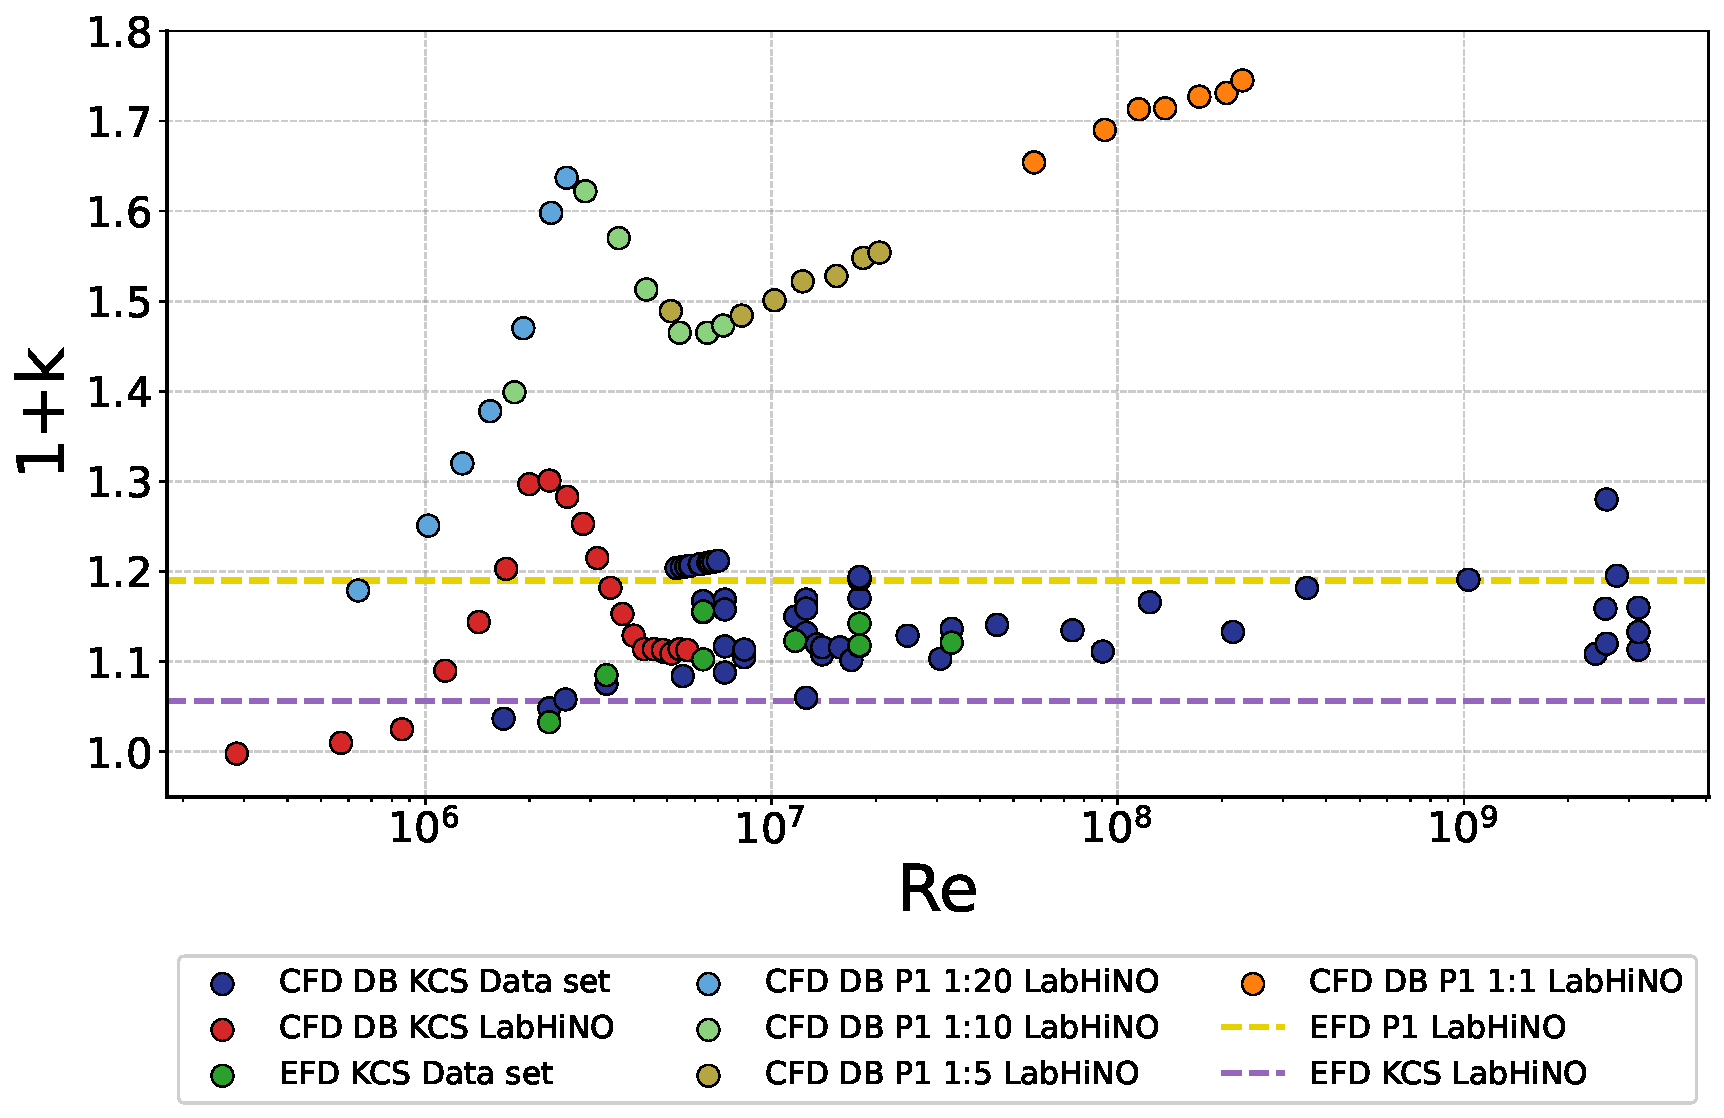
\includegraphics[height=2.9cm]{completo_log_kcs_lit_tpa.pdf}
  \begin{block}{Resistencia}
  \small $C_{PV}$ persiste con $Re$ $\Rightarrow$ $\uk$ crece sin asíntota ($k_S-k_M=0.52$). El ITTC supone $k_M=k_S$.
  \end{block}
\column{0.49\textwidth}
  \centering
  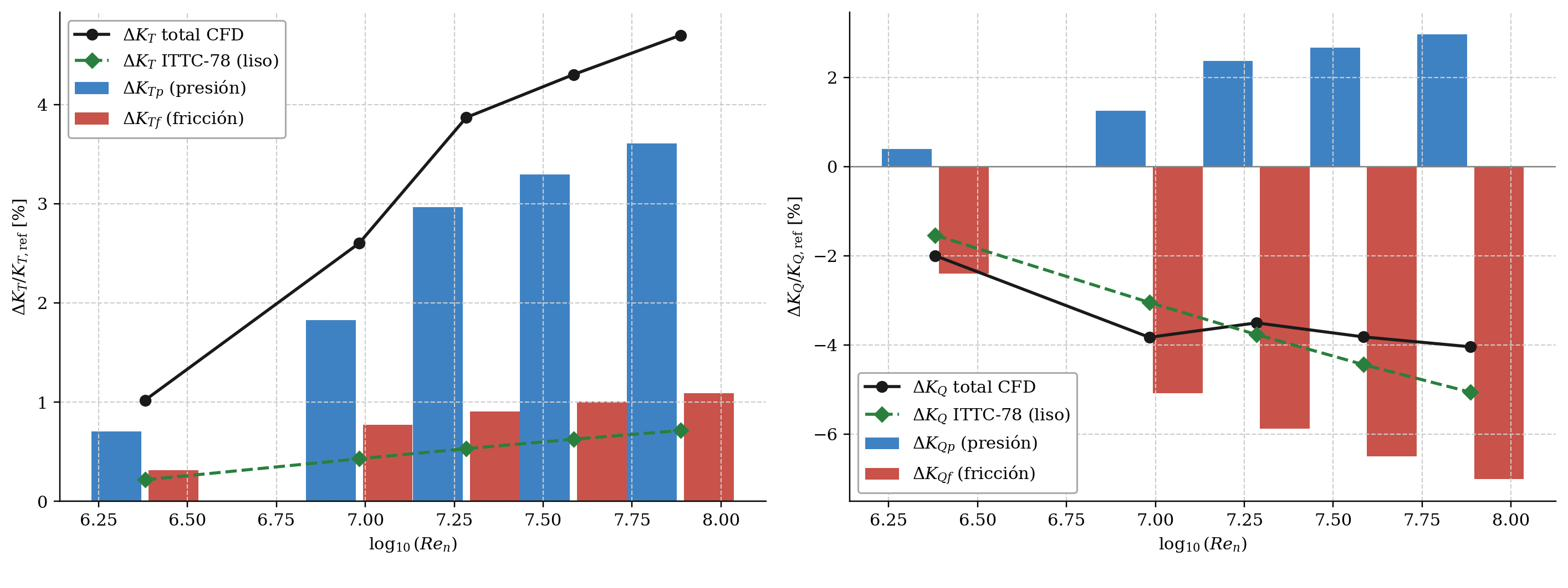
\includegraphics[height=2.6cm]{fig2_delta_descomp.png}
  \begin{block}{Propulsión}
  \small 76–77\,\% (\Bfs) y 90–92\,\% (\Pdos) del efecto de escala sobre $K_T$ es de presión. El ITTC-78 supone $\Delta K_{Tp}=0$.
  \end{block}
\end{columns}
\mensaje{Los procedimientos estándar corrigen la \textbf{fracción menor} del fenómeno y omiten la mayor.}
\note{1 min. Cerrar la pregunta transversal planteada al inicio.}
\end{frame}

\begin{frame}{Aportes principales}
\small
\begin{enumerate}
  \item Primera caracterización, con datos propios y en tres cascos, del efecto de escala de $\uk$ en pesqueros de \alert{baja esbeltez}: crecimiento continuo y no asintótico hasta escala buque.
  \item Identificación de la \alert{presión viscosa de popa} como causa dominante, y cuantificación y descarte de bulbo, popa sumergida y línea de fricción.
  \item Propuesta de \alert{correlaciones aerodinámicas en función de $L/B$} como marco para estimar $\uk$.
  \item Cuantificación de la \alert{fracción de presión} del efecto de escala en hélices: 76–77\,\% (\Bfs) y 90–92\,\% (\Pdos).
  \item Caracterización EFD–CFD de la \alert{joroba transicional} y de su impacto sobre la extrapolación ITTC-78.
  \item Evaluación del impacto en potencia: \alert{13–17\,\%} en $P_E$; métodos de doble $k$ y correcciones de presión.
  \item Metodología combinada \alert{EFD–CFD} consolidada y validada frente a referencias internacionales.
\end{enumerate}
\note{1 min.}
\end{frame}

\begin{frame}{Líneas futuras}
\begin{columns}[T]
\column{0.49\textwidth}
\begin{block}{Resistencia}
\small
\begin{itemize}
  \item Correlación $\uk = f(L/B)$ calibrada para $L/B<4$ con más geometrías.
  \item Validación con \alert{pruebas de mar}.
  \item Condición autopropulsada: interacción casco–hélice.
\end{itemize}
\end{block}
\column{0.49\textwidth}
\begin{block}{Propulsión}
\small
\begin{itemize}
  \item Mapeo de $f_p$ con $Z$, $A_E/A_0$, skew y cuerdas.
  \item Turbuladores o rugosidad controlada para evitar la joroba en el ensayo.
  \item Forma funcional $f_p(Re)$ e incorporación de correcciones de presión a la extrapolación.
\end{itemize}
\end{block}
\end{columns}
\note{1 min. Terminar con: “un esquema de extrapolación que no suponga que el efecto de escala es puramente friccional”.}
\end{frame}

\begin{frame}[standout]
¡Muchas gracias!\\[1em]
{\normalsize Preguntas}\\[1.5em]
{\scriptsize\mdseries Publicación asociada: Oyuela et al. (2024), \textit{Journal of Marine Science and Engineering}.}
\end{frame}

% =====================================================================
%  RESPALDO
% =====================================================================
\appendix
\begin{frame}[standout]
Diapositivas de respaldo
\end{frame}

\begin{frame}{Respaldo · Ajustes de York sobre el diagrama de Prohaska}
\begin{columns}[T]
\column{0.49\textwidth}
  \centering
  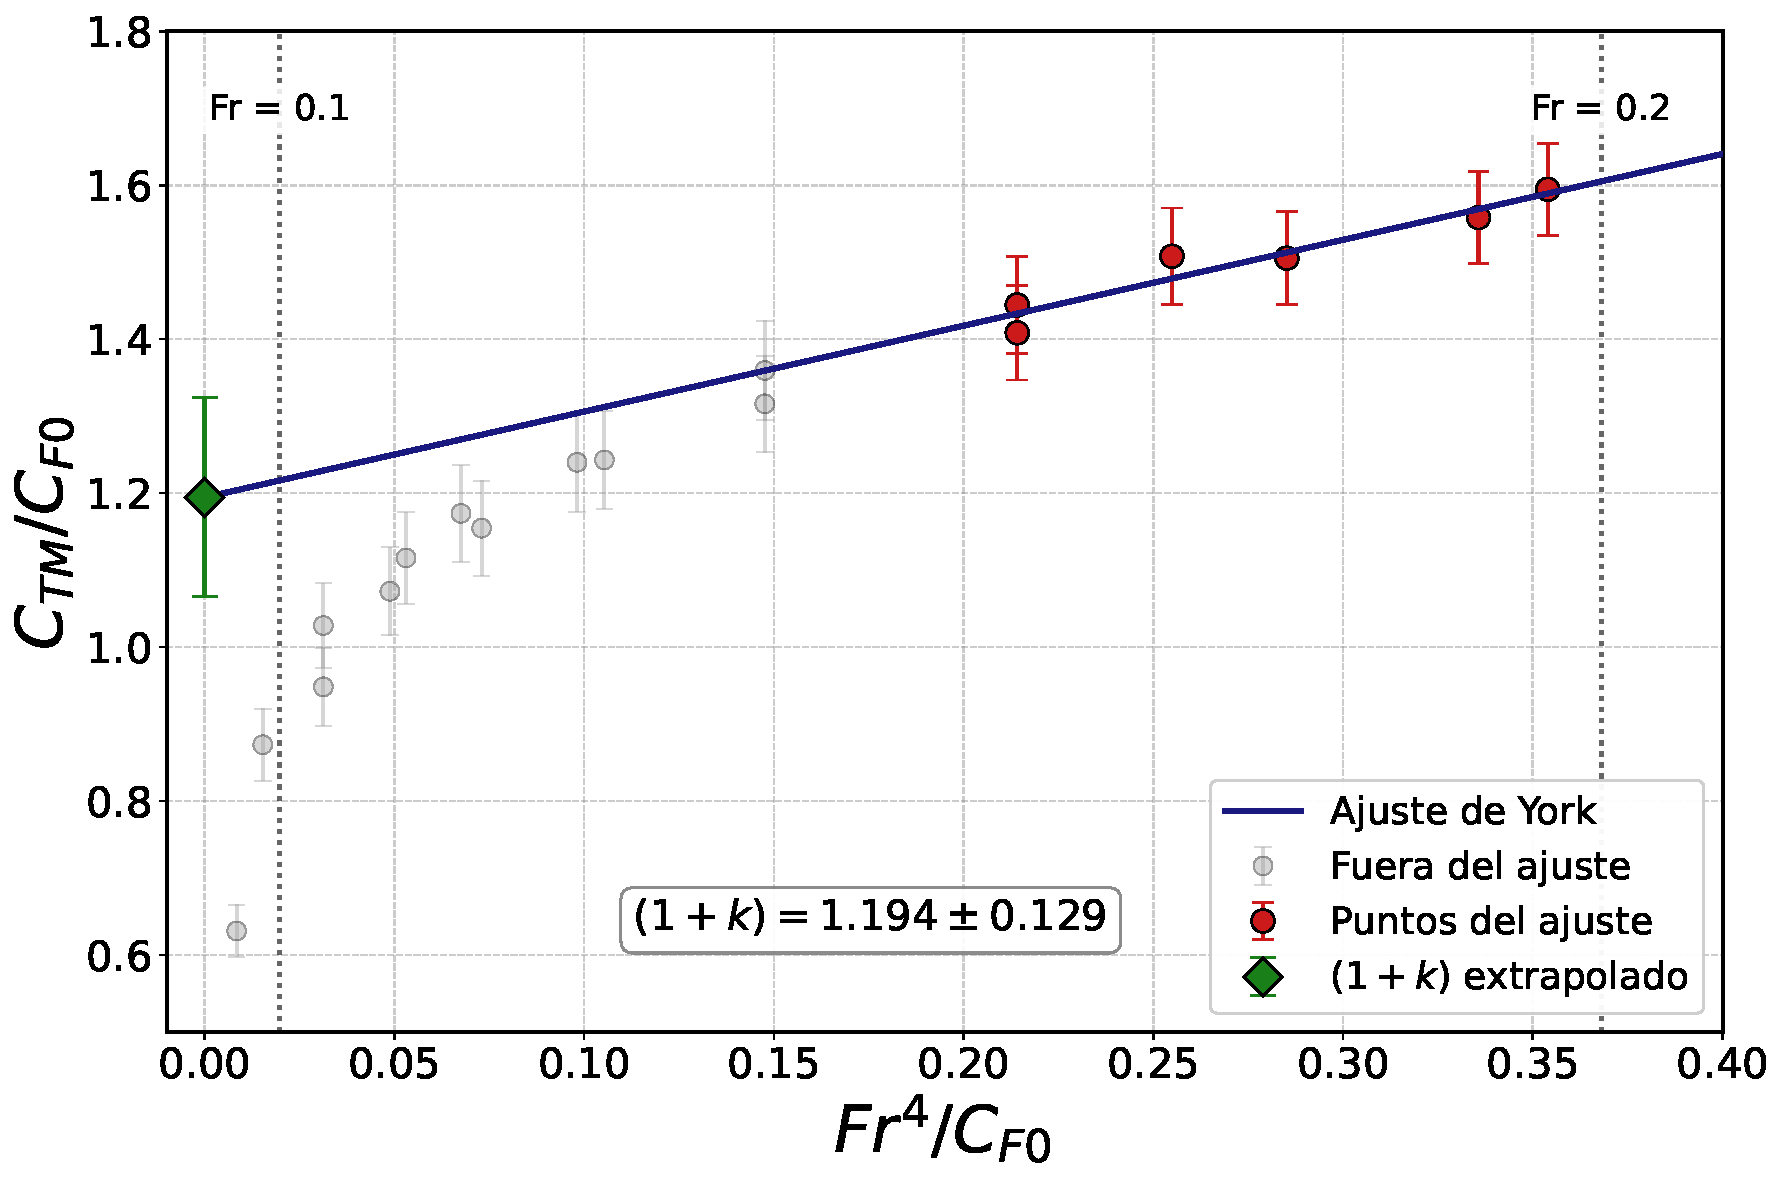
\includegraphics[width=0.82\linewidth]{york_tpa_180.pdf}\\
  \small \Pu, T2
\column{0.49\textwidth}
  \centering
  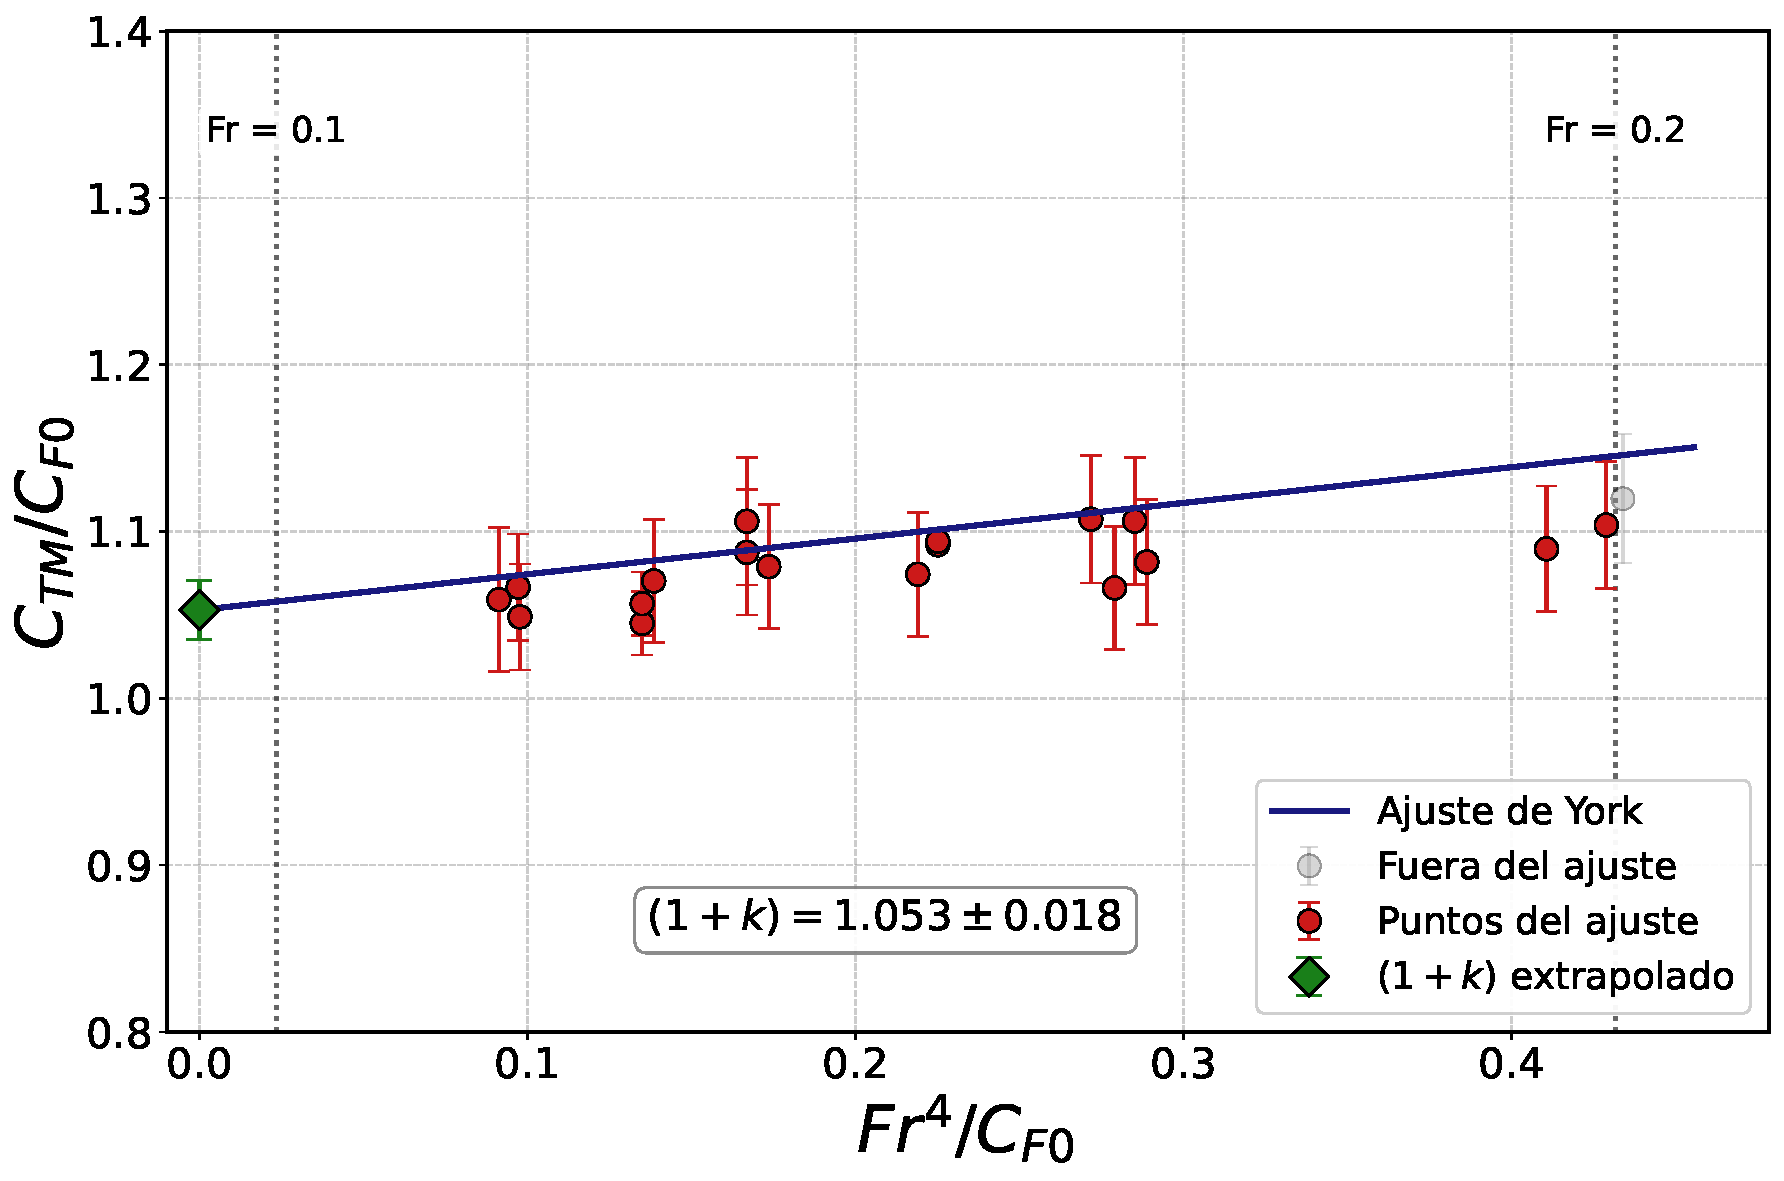
\includegraphics[width=0.82\linewidth]{york_kcs.pdf}\\
  \small \KCS
\end{columns}
\vspace{0.4em}
\centering\small
\begin{tabular}{lccc}
\toprule
\Pu & T1 & T2 & T3 \\
\midrule
$\uk$ & 1.235 & 1.194 & 1.190 \\
$U(1+k)/(1+k)$ & $\pm8.4\,\%$ & $\pm10.8\,\%$ & $\pm11.2\,\%$ \\
\bottomrule
\end{tabular}
\end{frame}

\begin{frame}{Respaldo · Validación EFD–CFD en los otros calados}
\begin{columns}[T]
\column{0.49\textwidth}
  \centering
  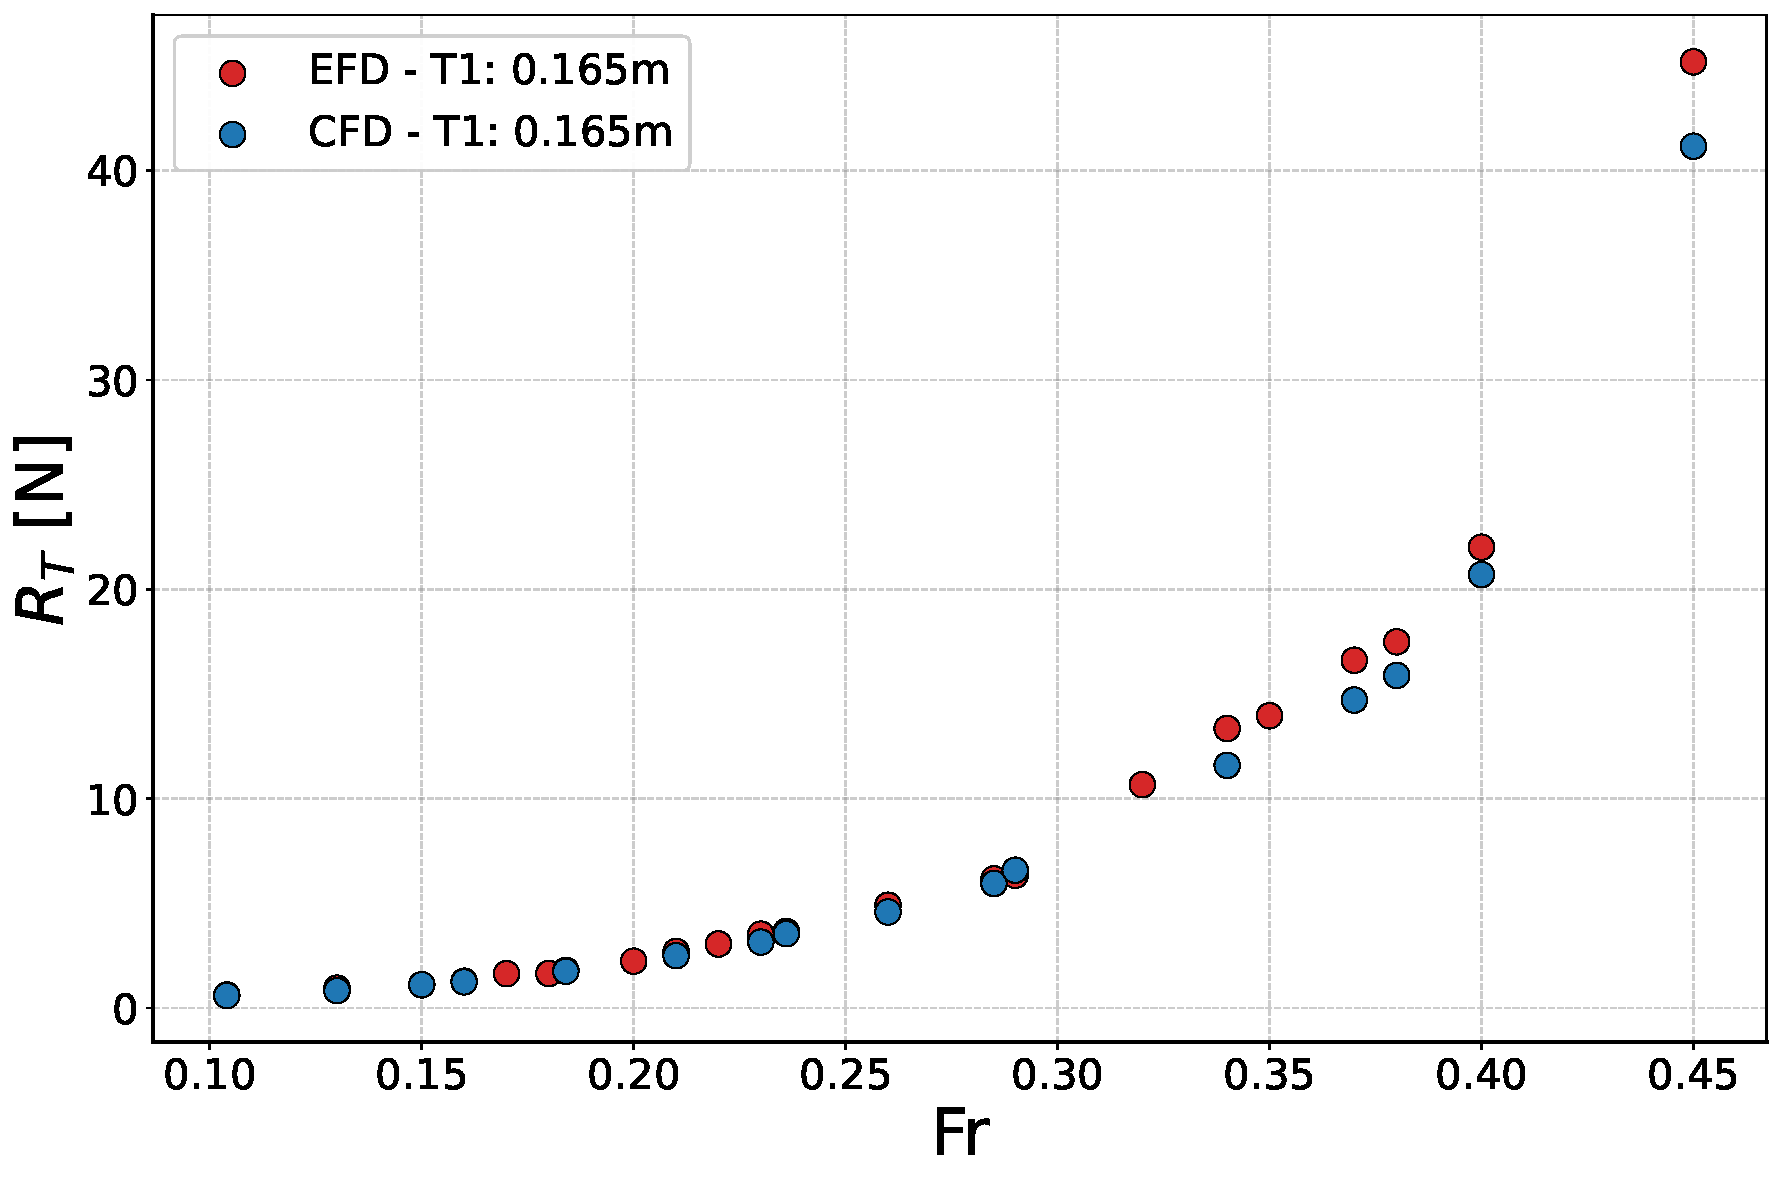
\includegraphics[width=\linewidth]{efd_cfd_165.pdf}\\
  \small T1 (0.165\,m): error medio $\sim$5\,\% en el rango operativo.
\column{0.49\textwidth}
  \centering
  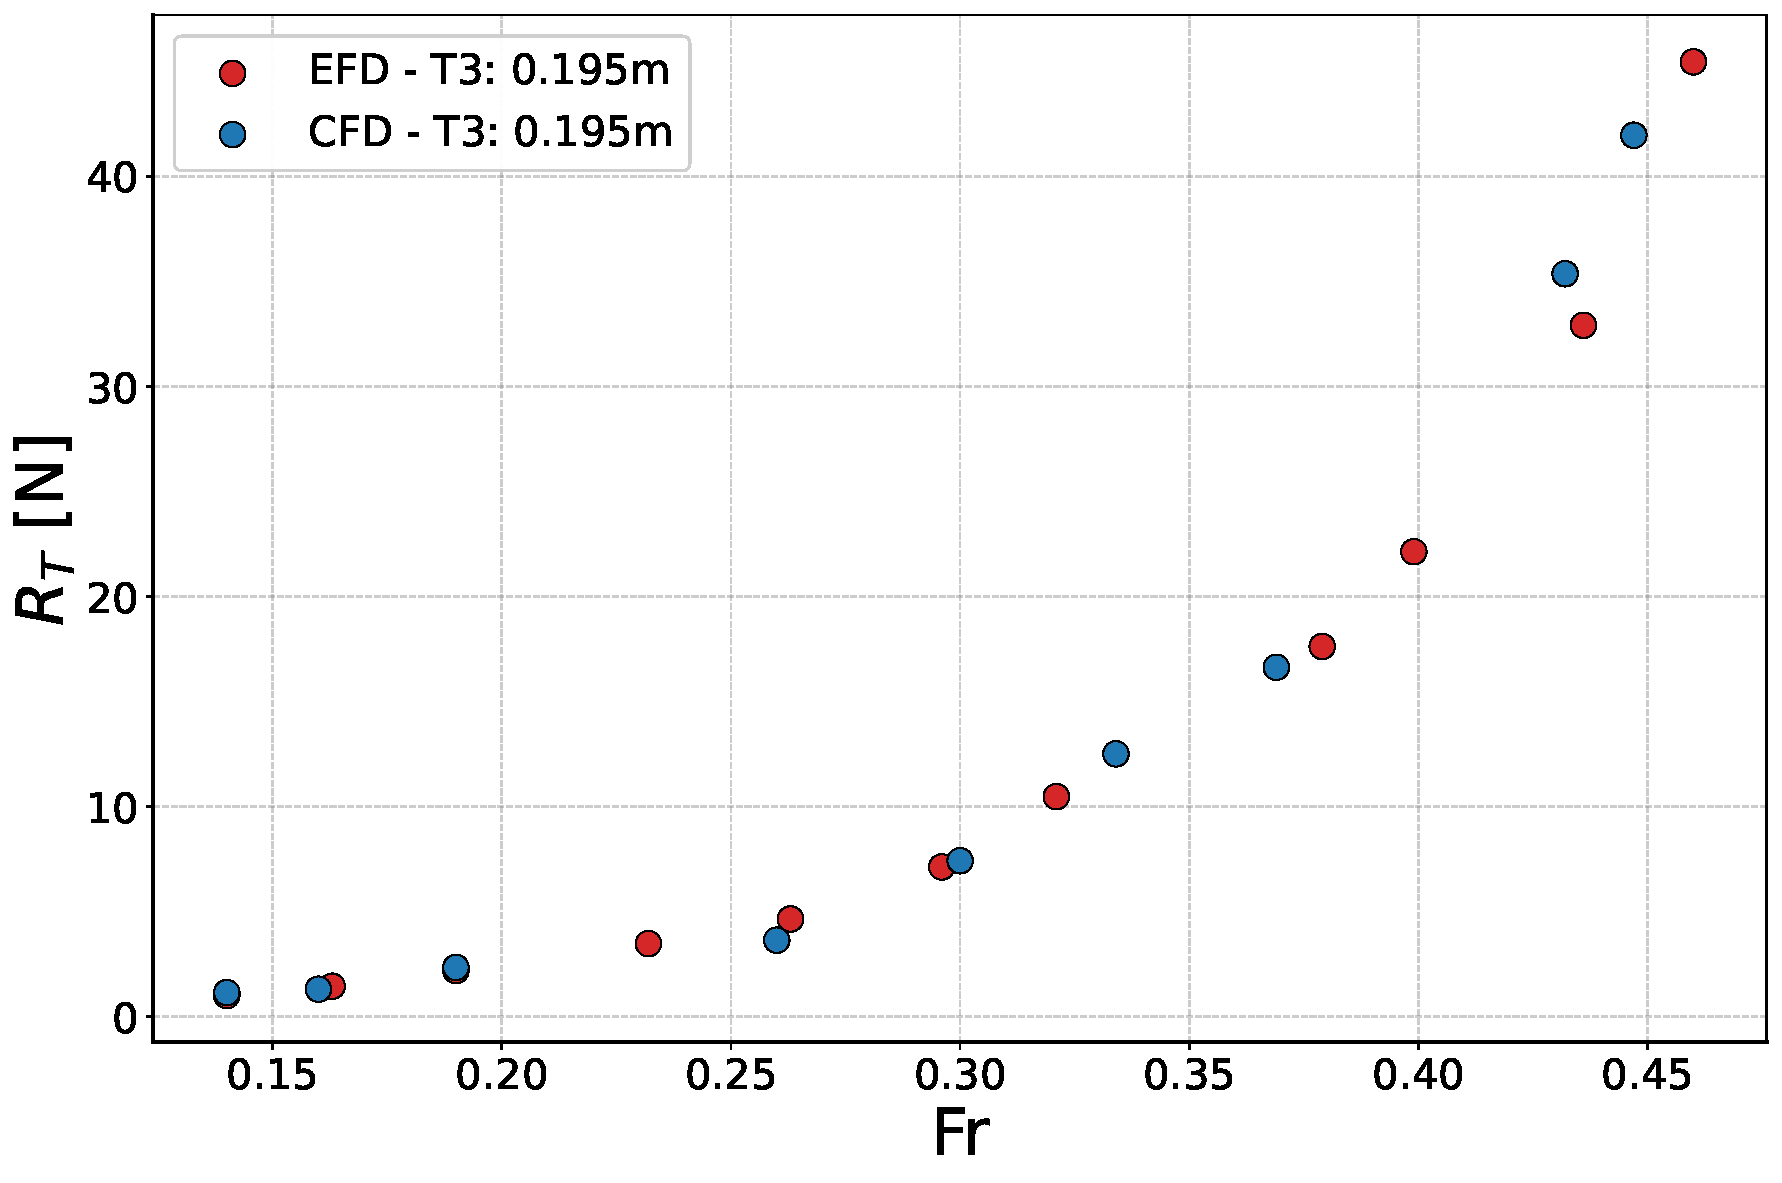
\includegraphics[width=\linewidth]{efd_cfd_195.pdf}\\
  \small T3 (0.195\,m): concordancia de 1–2\,\% (CFD interpolado a las $Fr$ ensayadas).
\end{columns}
\end{frame}

\begin{frame}{Respaldo · \KCS: comparación con la literatura}
\begin{columns}[T]
\column{0.49\textwidth}
  \centering
  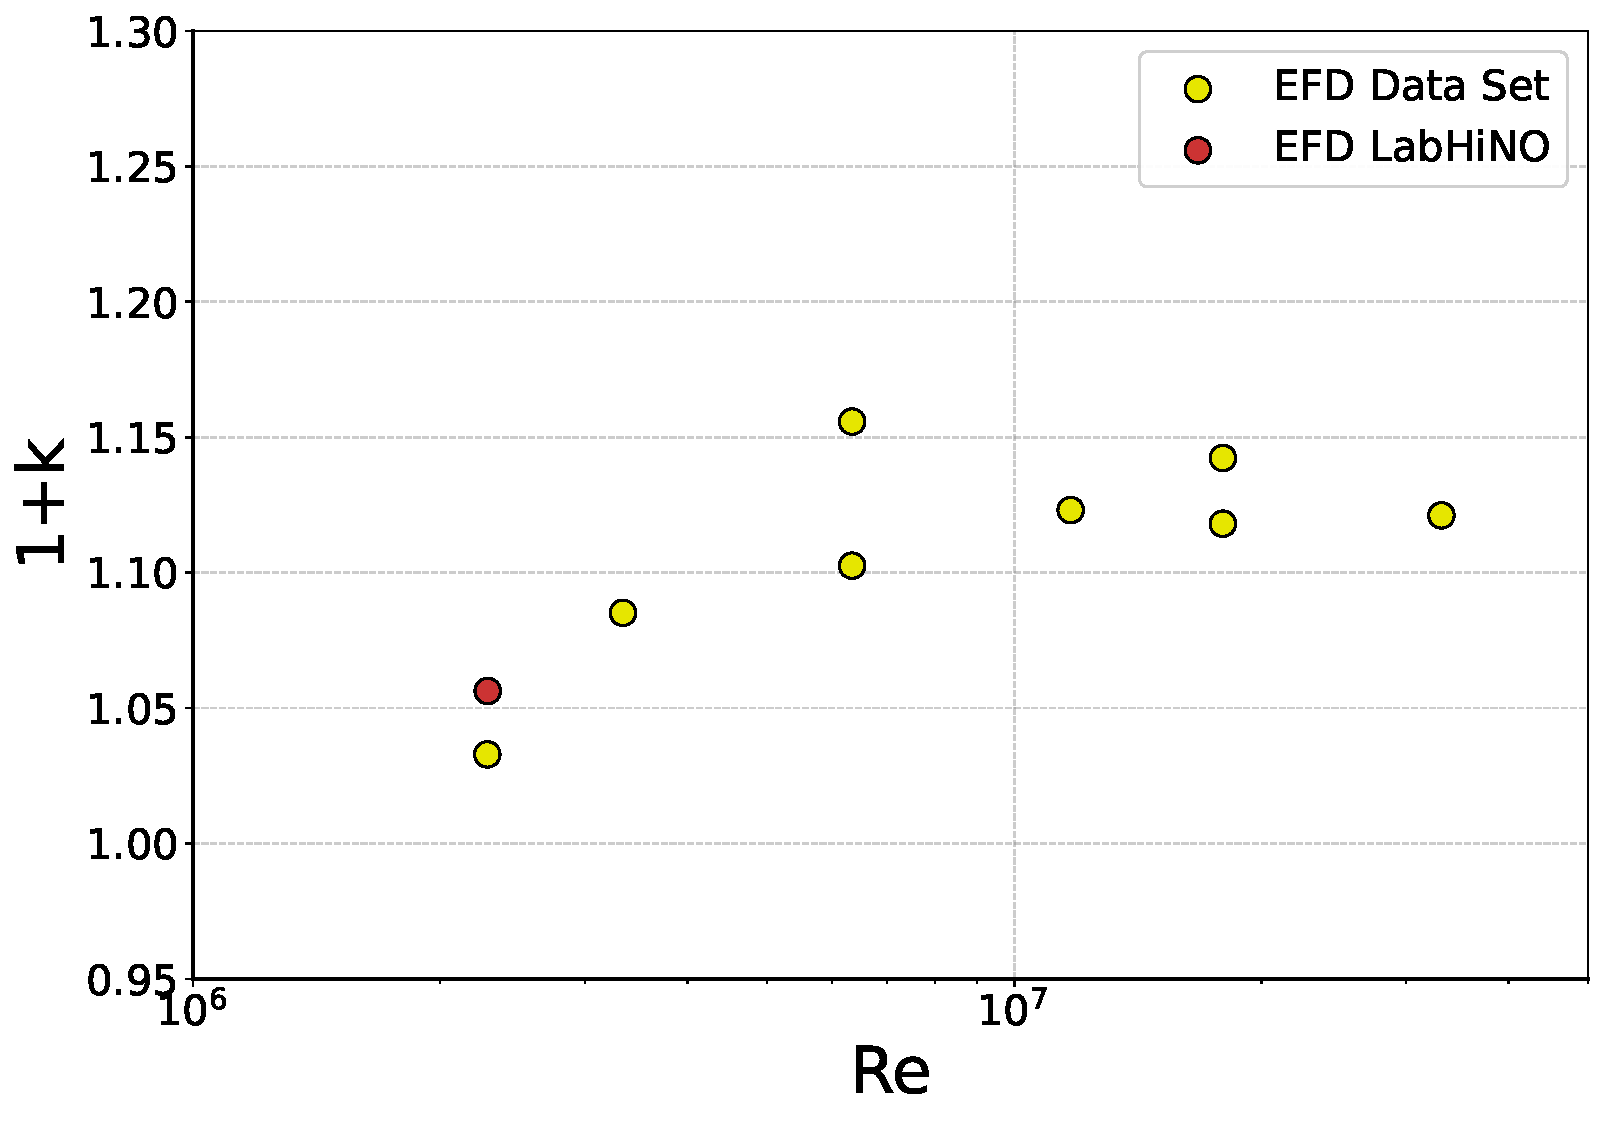
\includegraphics[width=\linewidth]{efd_kcs_lit.pdf}\\
  \small EFD propio frente a otros laboratorios.
\column{0.49\textwidth}
  \centering
  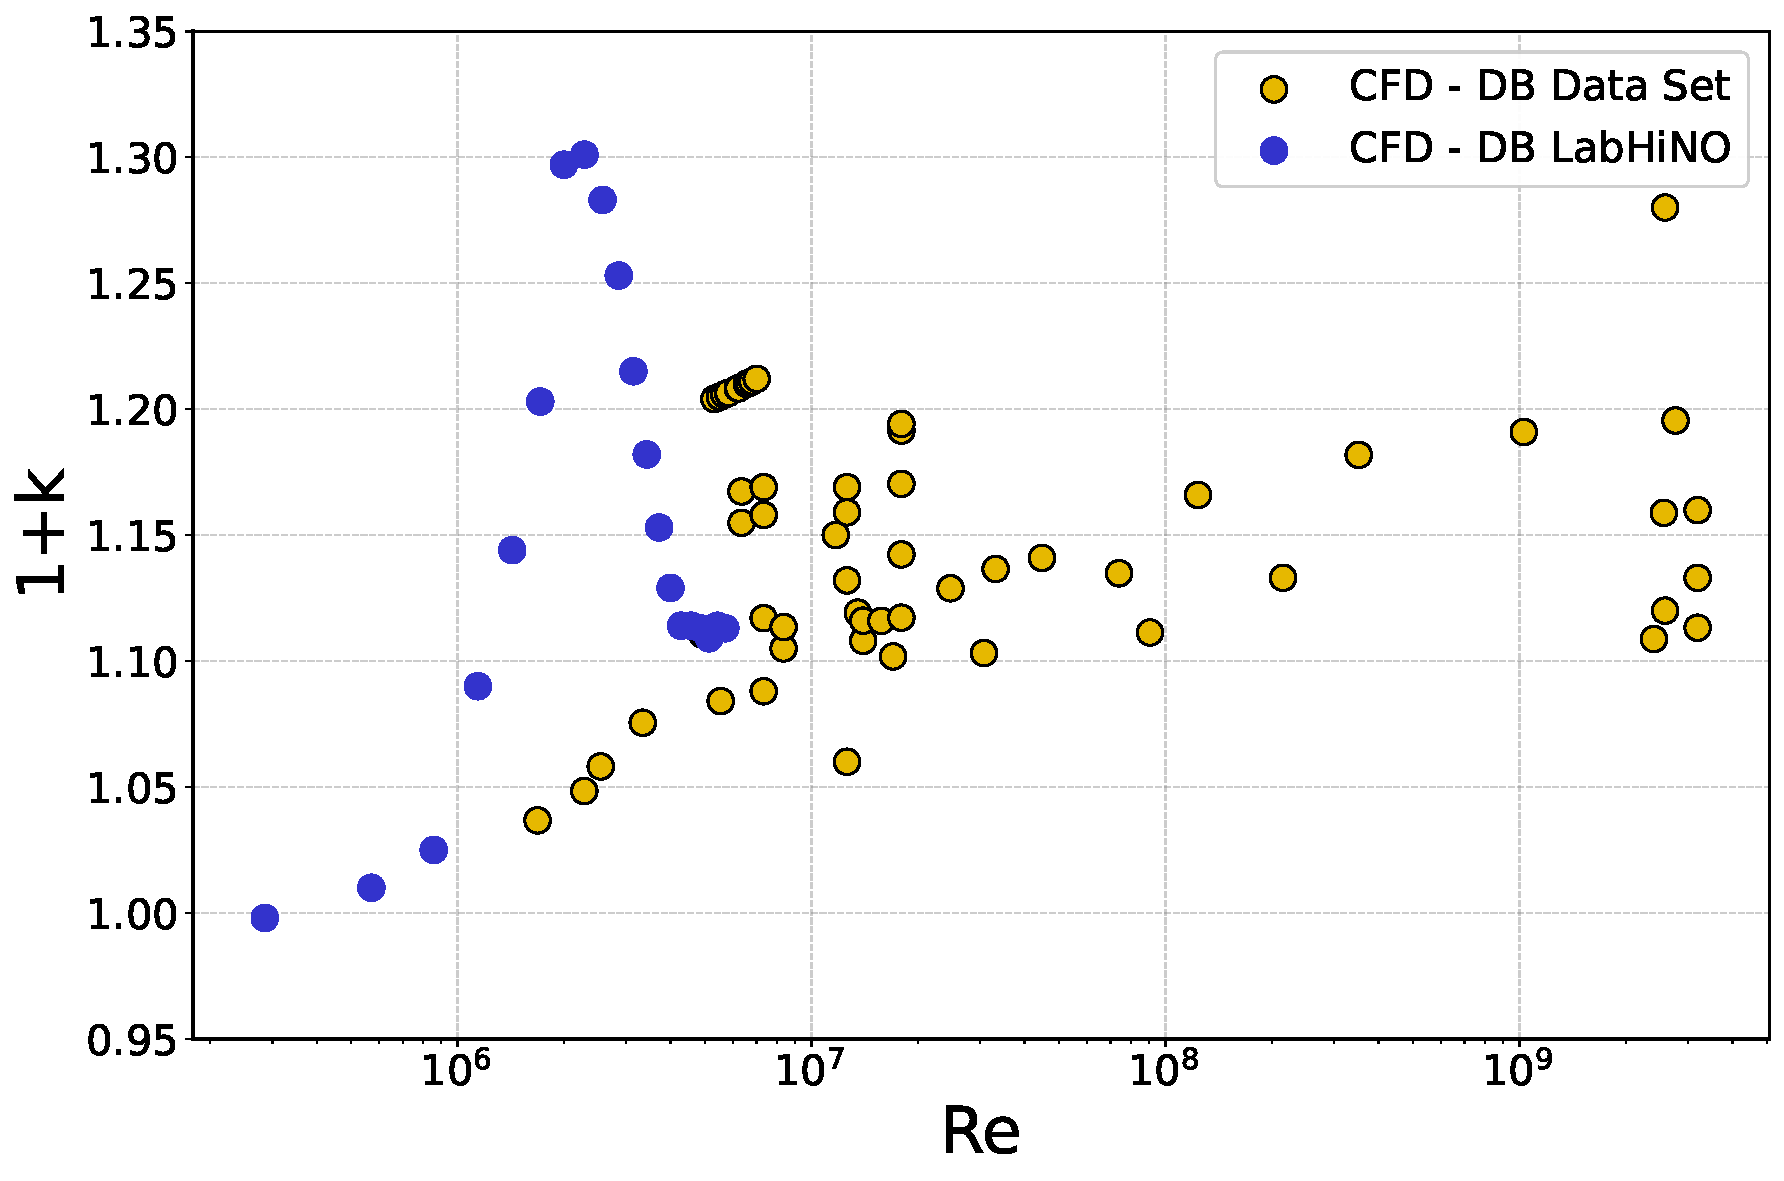
\includegraphics[width=\linewidth]{cfd_kcs_lit.pdf}\\
  \small CFD DB propio frente a la base de datos de Terziev et al.
\end{columns}
\end{frame}

\begin{frame}{Respaldo · Diagramas de Prohaska con y sin bulbo}
\begin{columns}[T]
\column{0.49\textwidth}
  \centering
  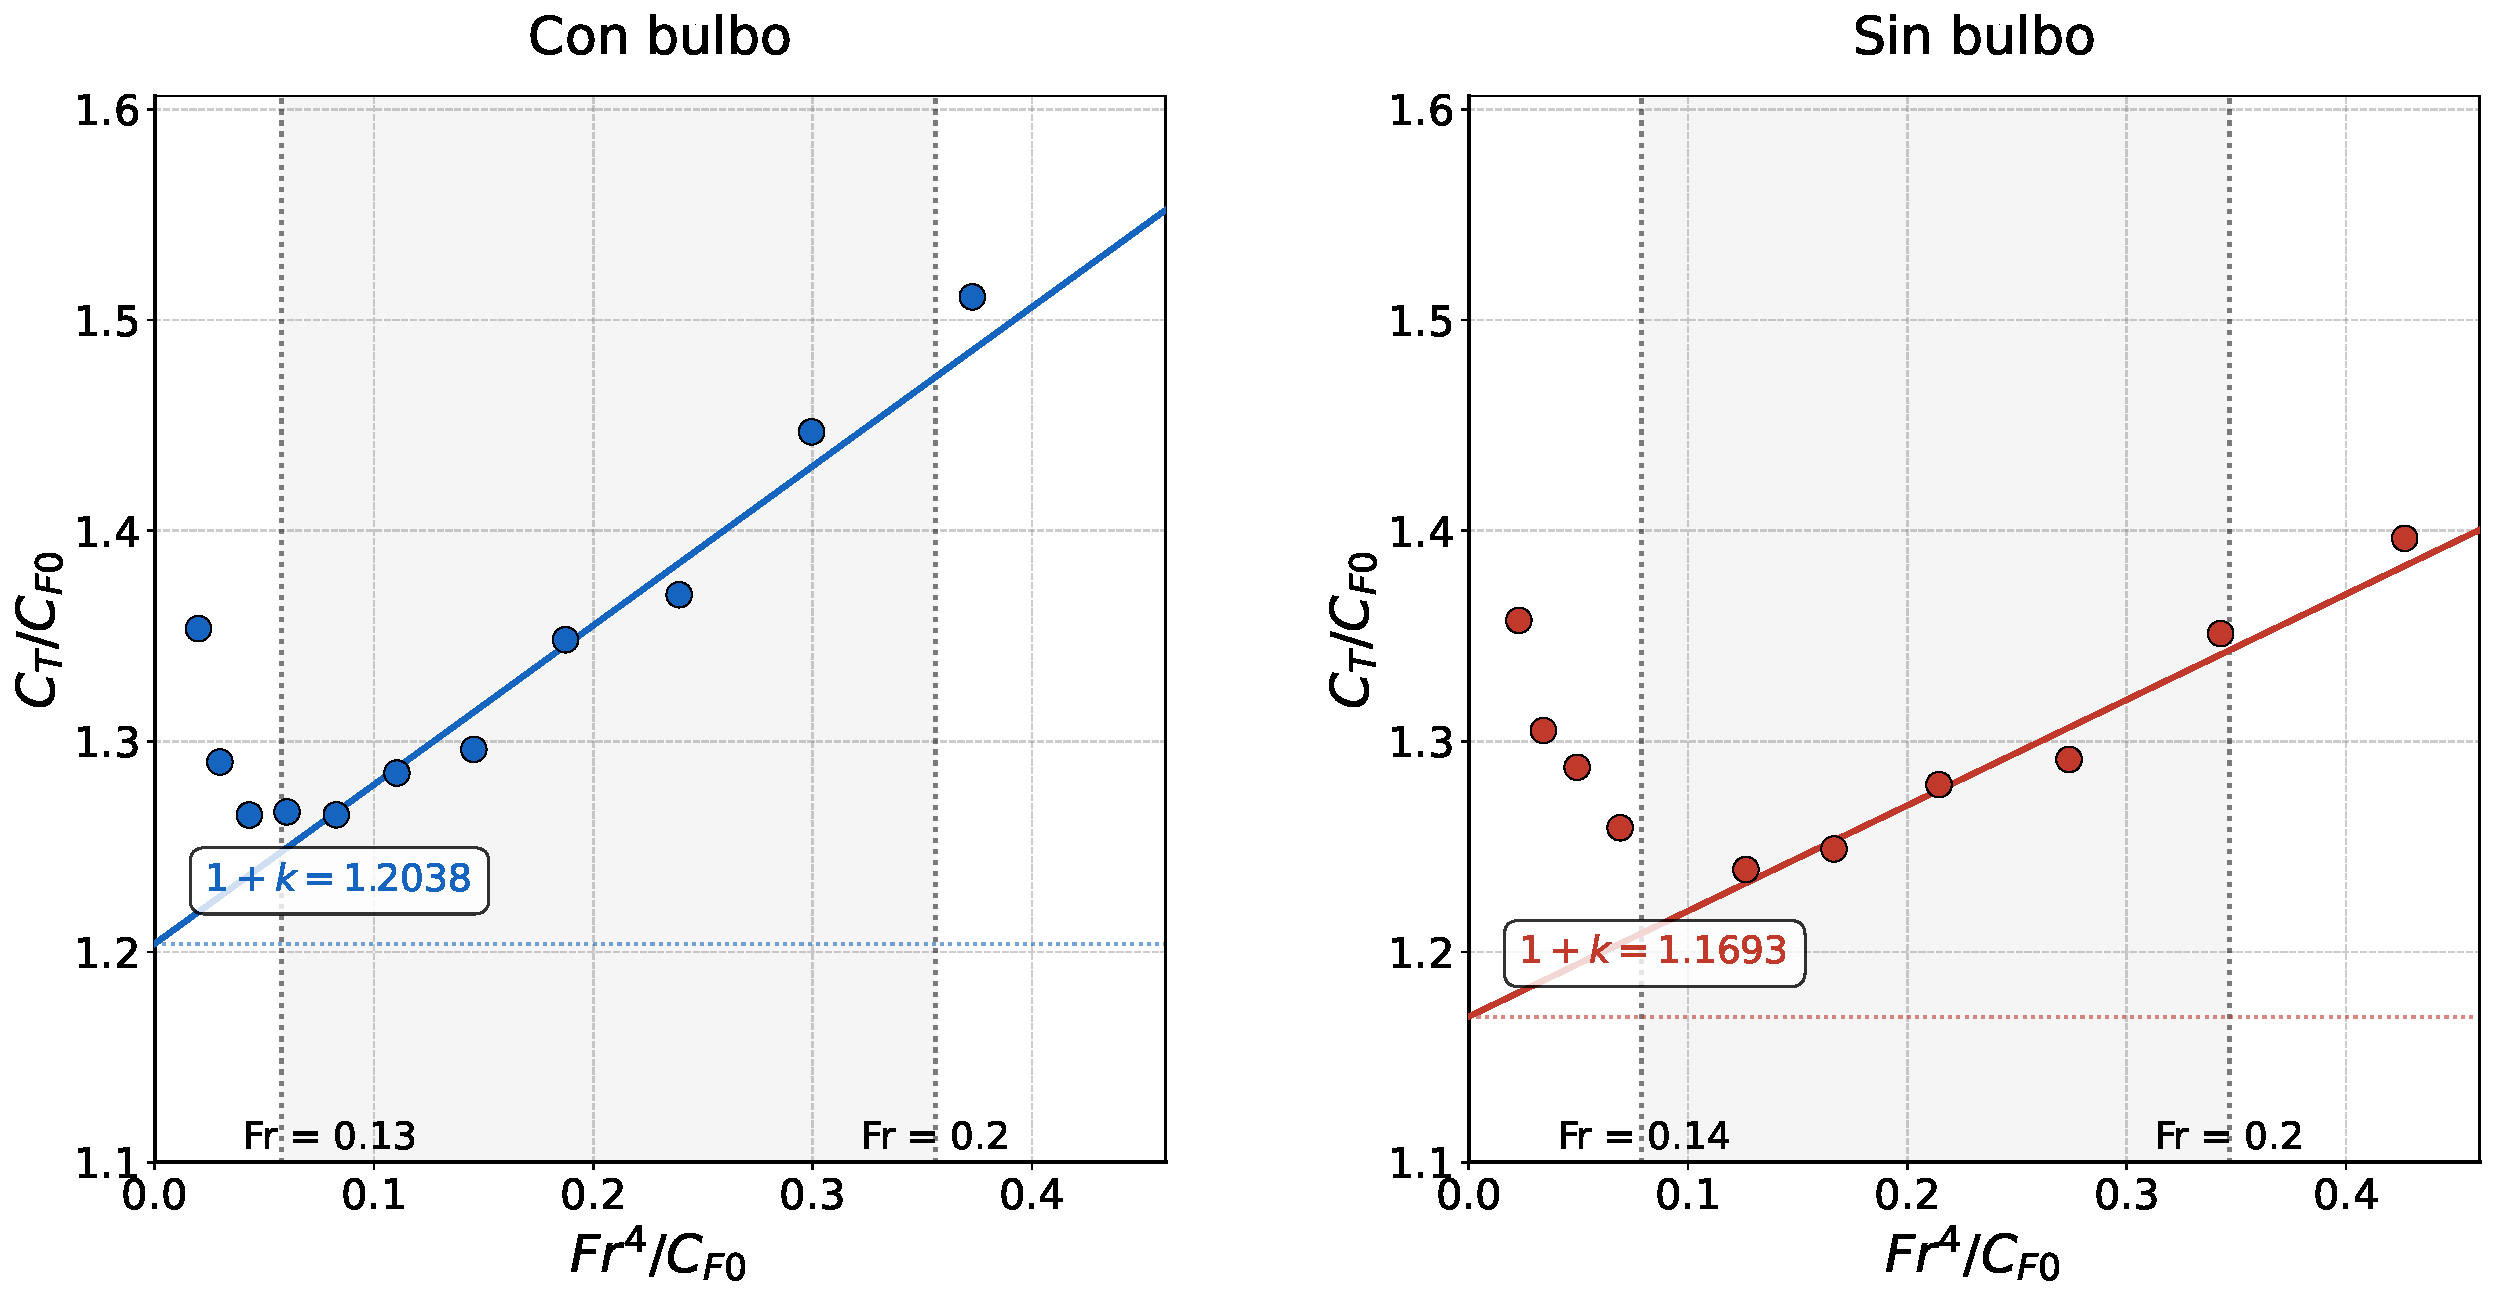
\includegraphics[width=\linewidth]{prohaska-bulbo-ctrlz-165.pdf}\\
  \small Calado T1
\column{0.49\textwidth}
  \centering
  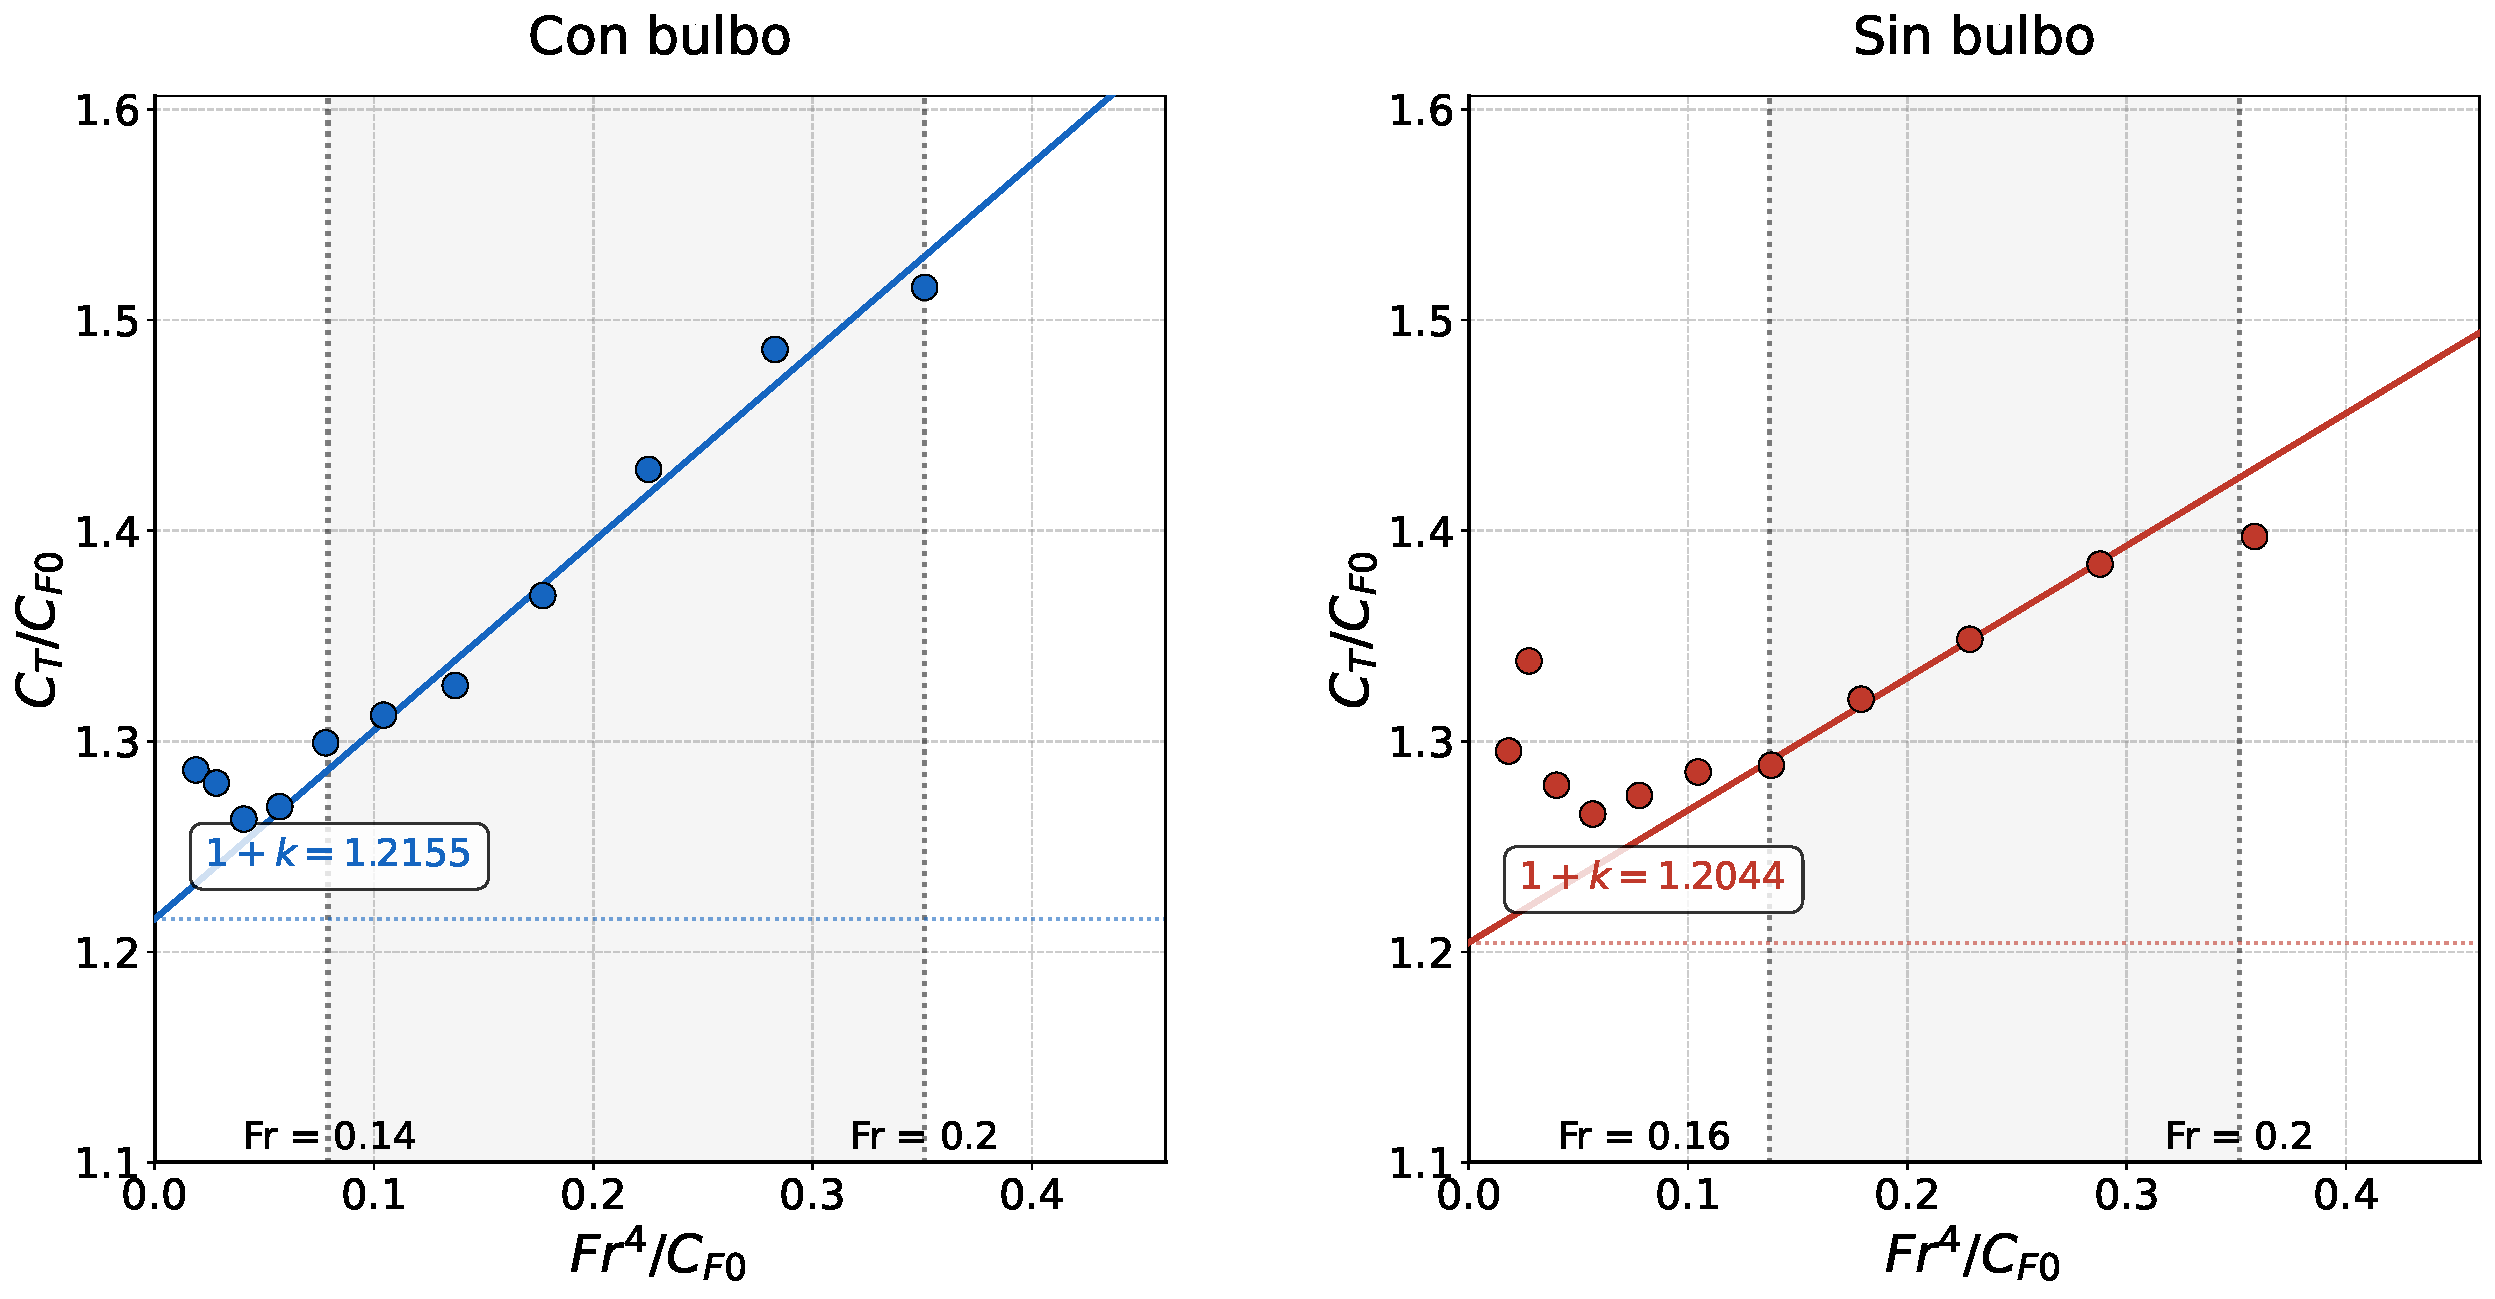
\includegraphics[width=\linewidth]{prohaska-bulbo-ctrlz-195.pdf}\\
  \small Calado T3
\end{columns}
\vspace{0.5em}
\small La curvatura a bajo $Fr$ persiste sin bulbo. El análisis no distingue entre un origen geométrico y uno asociado al modelado de la transición, porque ambas variantes usan el mismo modelo de turbulencia.
\end{frame}

\begin{frame}{Respaldo · Recirculación en la popa sumergida}
\begin{columns}[T]
\column{0.49\textwidth}
  \centering
  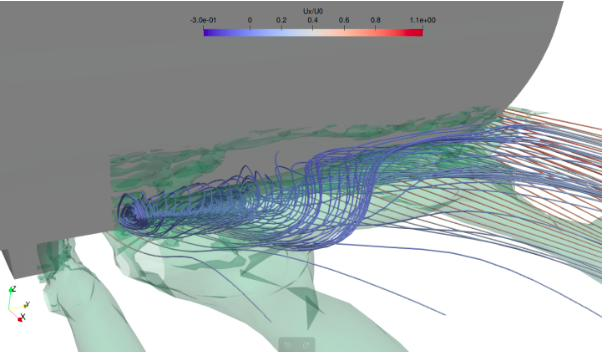
\includegraphics[width=\linewidth]{195-036-consup-modelo.png}\\
  \small Escala modelo
\column{0.49\textwidth}
  \centering
  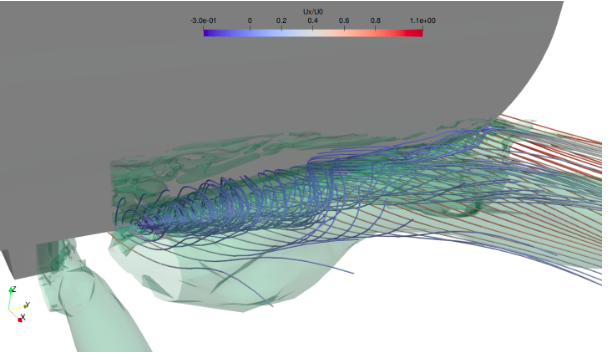
\includegraphics[width=\linewidth]{195-036-consup-real.png}\\
  \small Escala buque
\end{columns}
\vspace{0.5em}
\small La recirculación detrás del espejo se mantiene estable frente al cambio de escala, con y sin superficie libre: condición que justifica el método $2k$ (Korkmaz et al., 2022). Resultado: $k_{tr}=0.025$.
\end{frame}

\begin{frame}{Respaldo · Modelos de turbulencia: descomposición $C_F$ / $C_{PV}$}
\begin{columns}[T]
\column{0.49\textwidth}
  \centering
  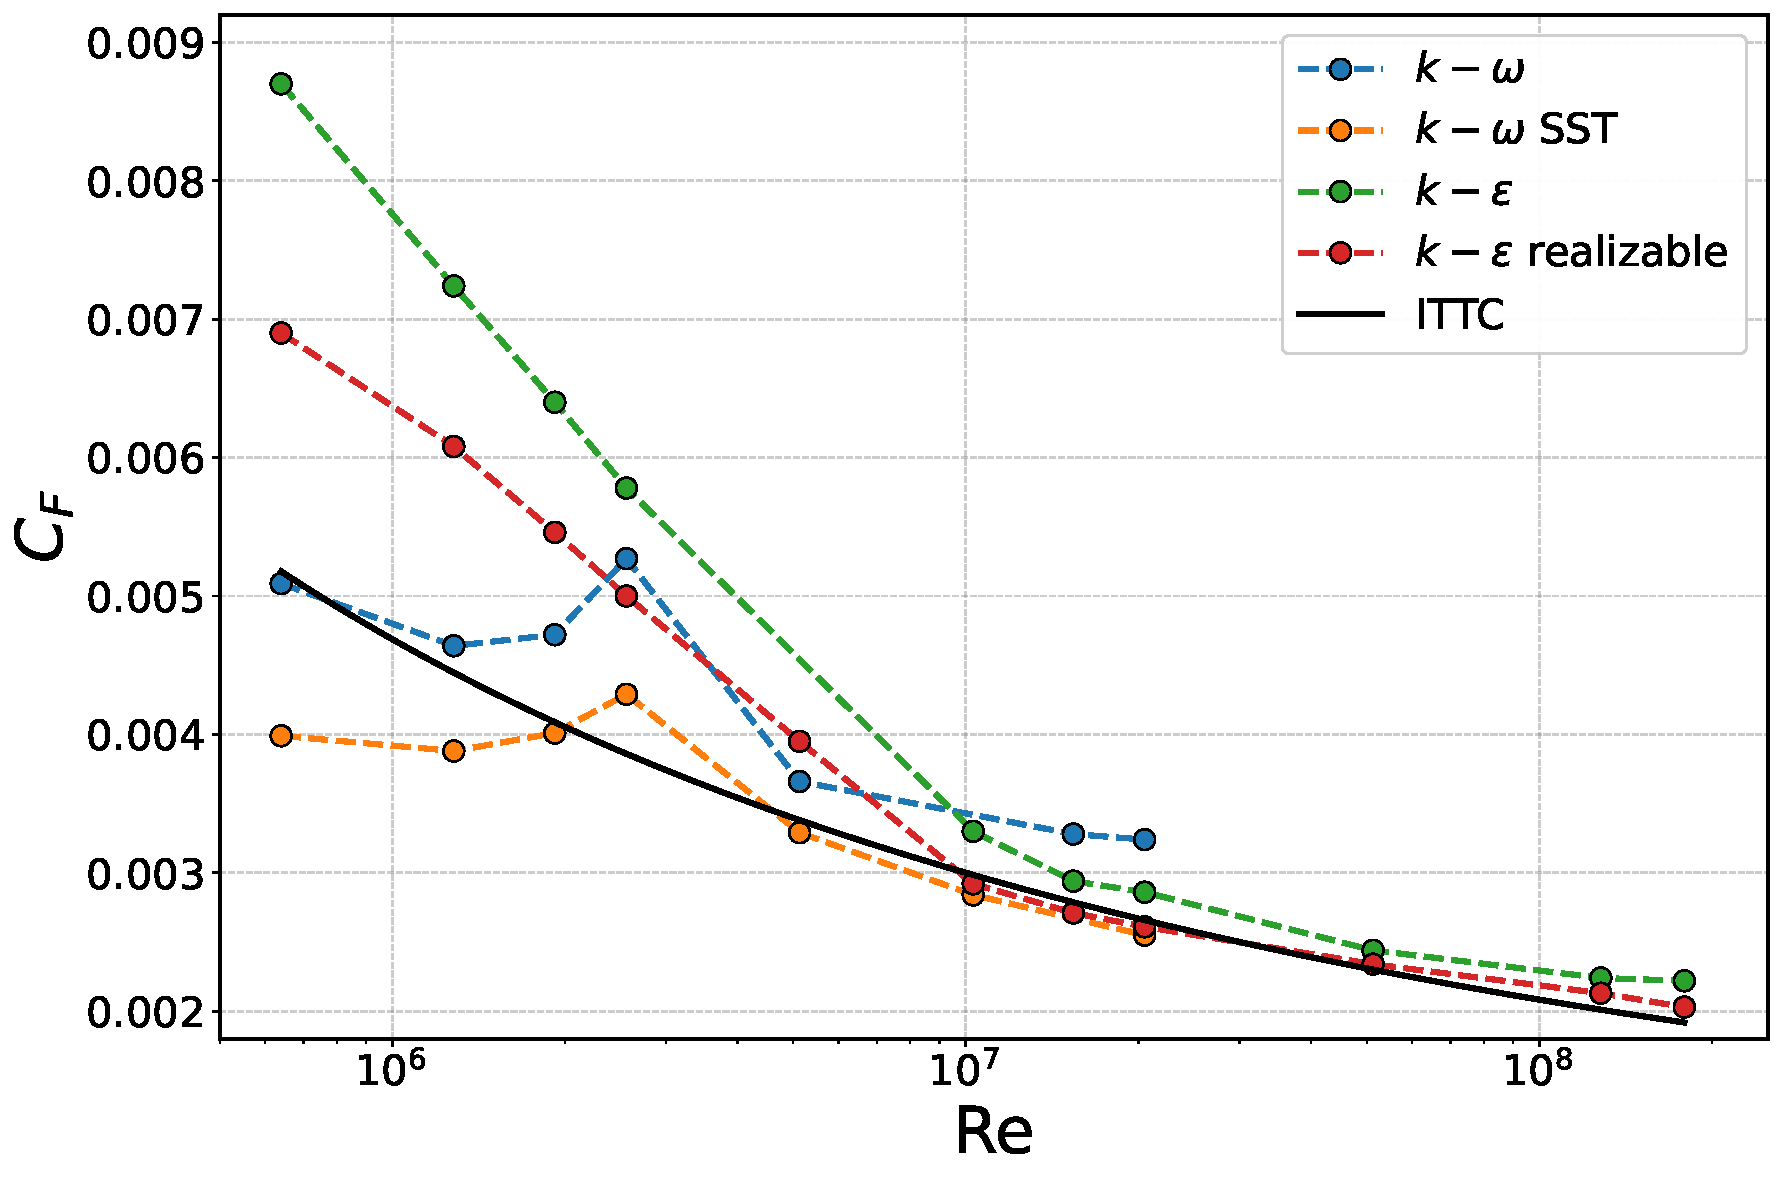
\includegraphics[width=\linewidth]{comparacion_cf.pdf}
\column{0.49\textwidth}
  \centering
  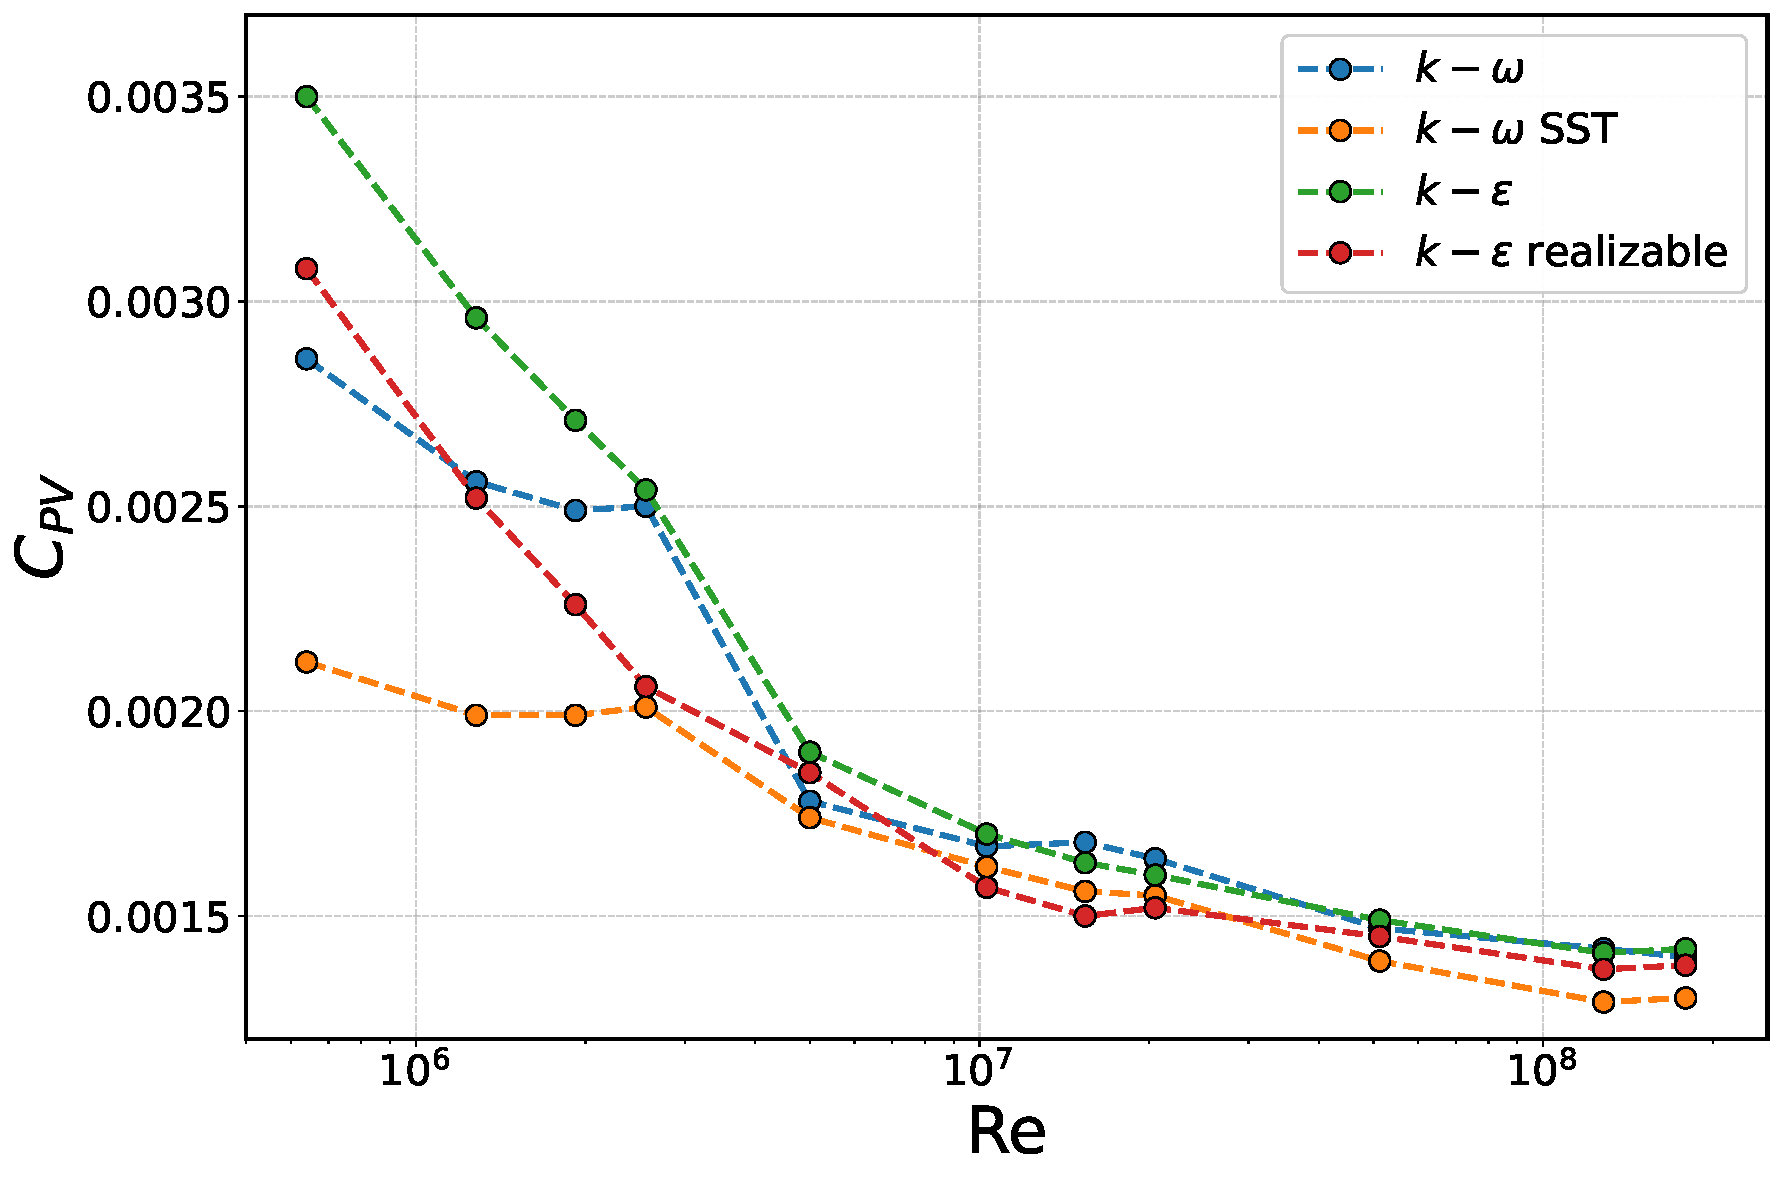
\includegraphics[width=\linewidth]{comparacion_cp.pdf}
\end{columns}
\vspace{0.4em}
\small A bajo $Re$ las diferencias afectan tanto a $C_F$ como a $C_{PV}$; la sensibilidad se atenúa al avanzar hacia régimen plenamente turbulento.
\end{frame}

\begin{frame}{Respaldo · Correlaciones navales en los cuatro cascos}
\centering
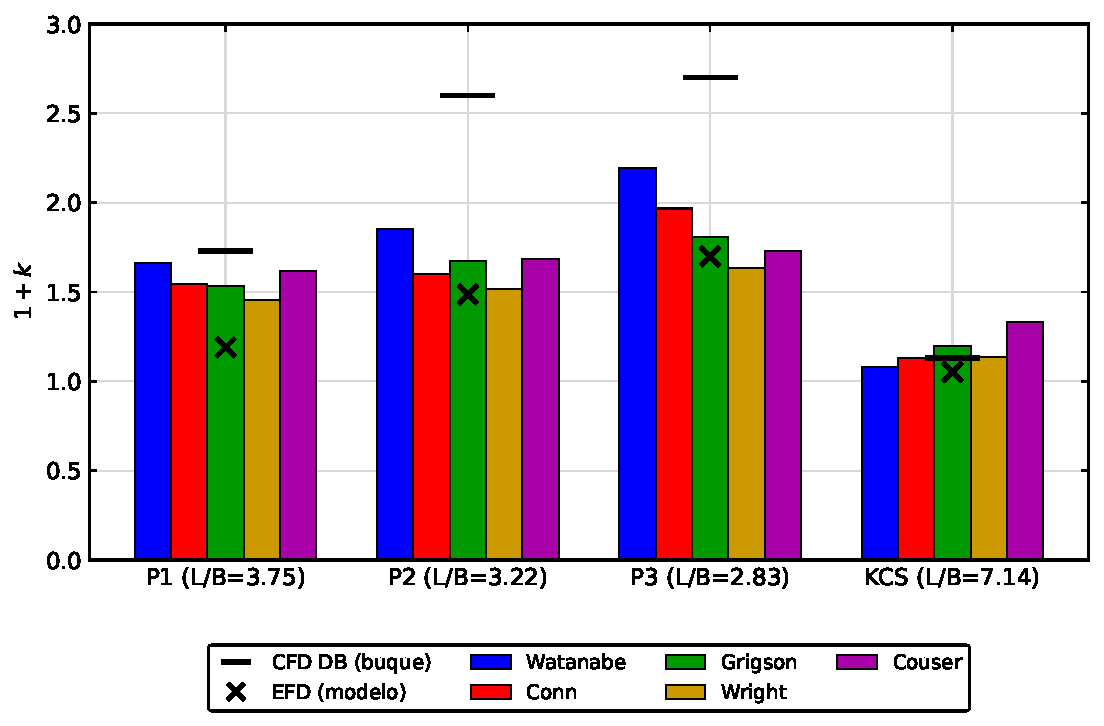
\includegraphics[height=5.6cm]{empiricas_4cascos.pdf}
\end{frame}

\begin{frame}{Respaldo · Tratamiento de pared y resolución}
\begin{itemize}
  \item $y^+$ desde $\sim$1 en las escalas de modelo hasta $>300$ a escala buque.
  \item Funciones de pared adaptativas de OpenFOAM (\texttt{kLowReWallFunction}, \texttt{omegaWallFunction}): integración hasta la pared con $y^+\approx1$ y ley logarítmica con $y^+>30$.
  \item Incertidumbre numérica en resistencia: $U_{num}<0.2\,\%$ en el rango operativo.
  \item Hélice \Bfs: GCI de $K_T$ = 1.39\,\%; malla fina de 8.4 M celdas (97.5\,\% hexaédricas).
\end{itemize}
\end{frame}

\begin{frame}{Respaldo · \Bfs: $\Delta K_T$ y $\Delta K_Q$ con el diámetro}
\centering
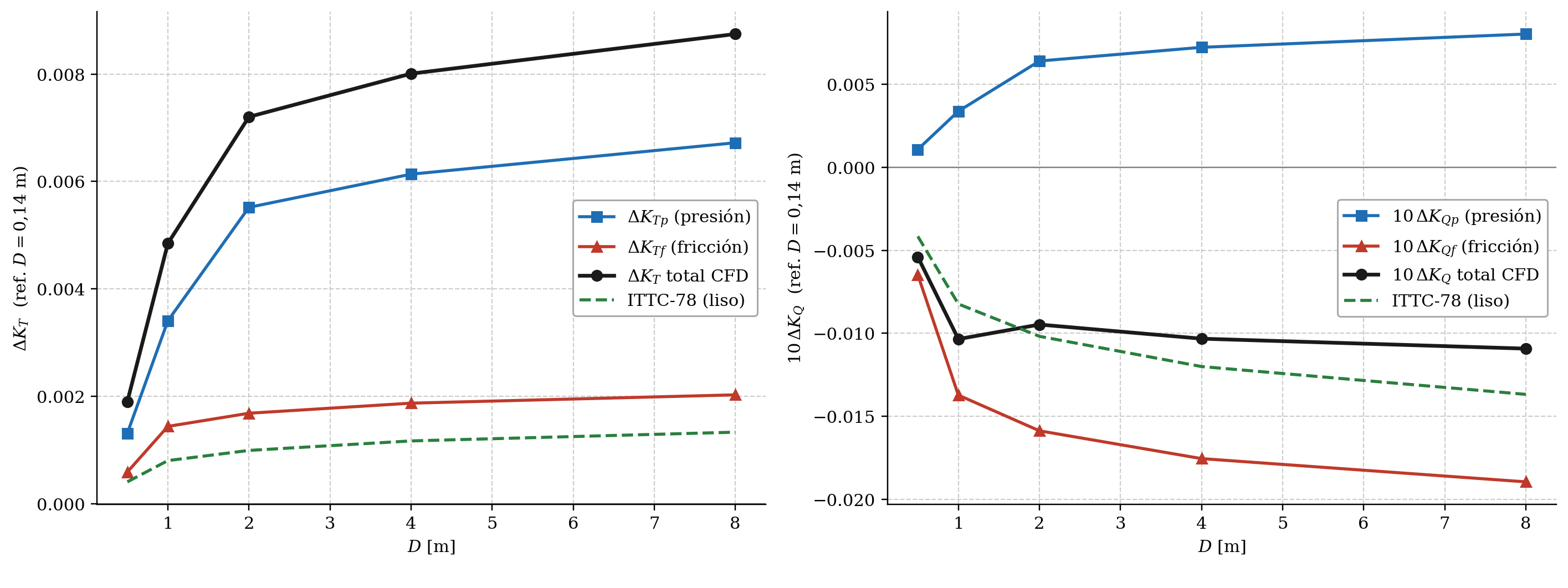
\includegraphics[height=2.85cm]{fig3_delta_vs_D.png}\\[0.3em]
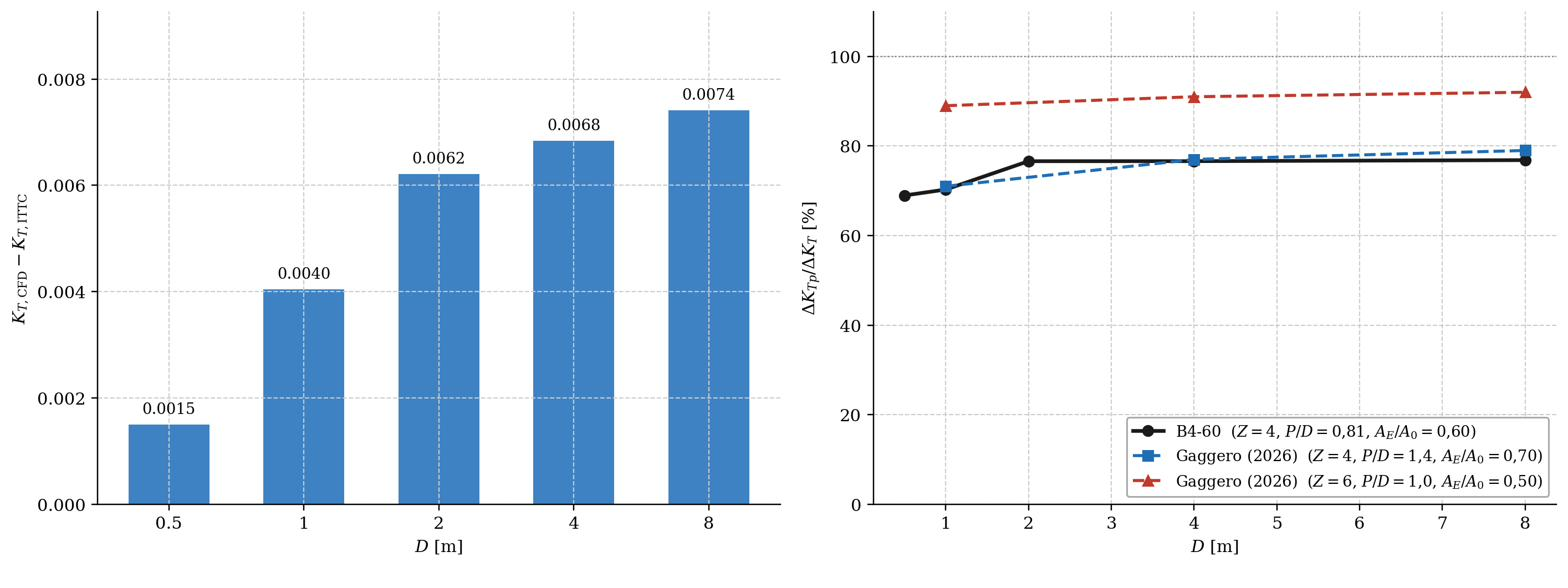
\includegraphics[height=2.85cm]{fig4_gap_fraccion.png}
\end{frame}

\begin{frame}{Respaldo · \Bfs: amplitud radial de la redistribución de presión}
\begin{columns}[c]
\column{0.55\textwidth}
  \centering
  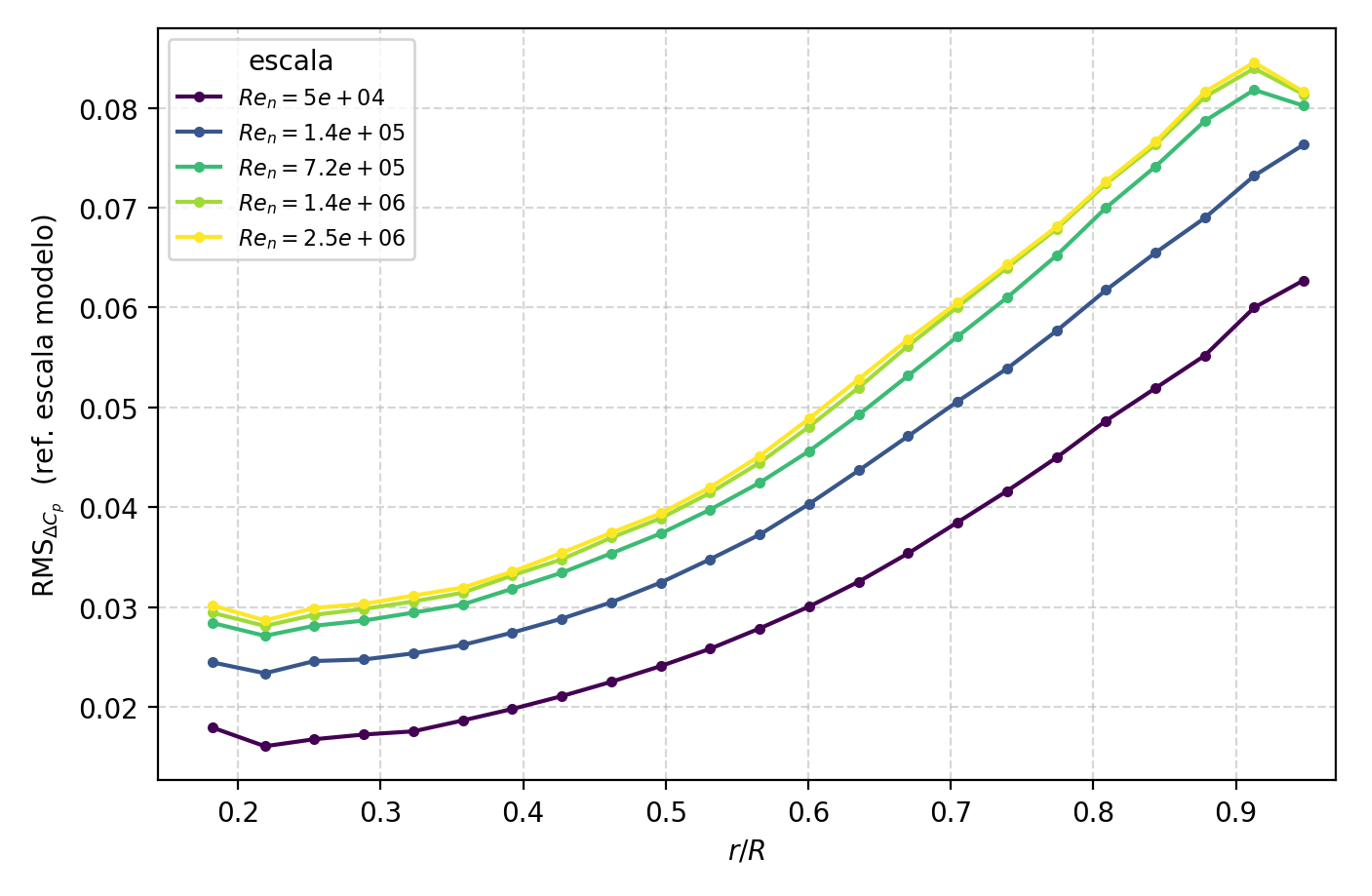
\includegraphics[width=\linewidth]{radial_rms_dcp.png}
\column{0.43\textwidth}
  \centering
  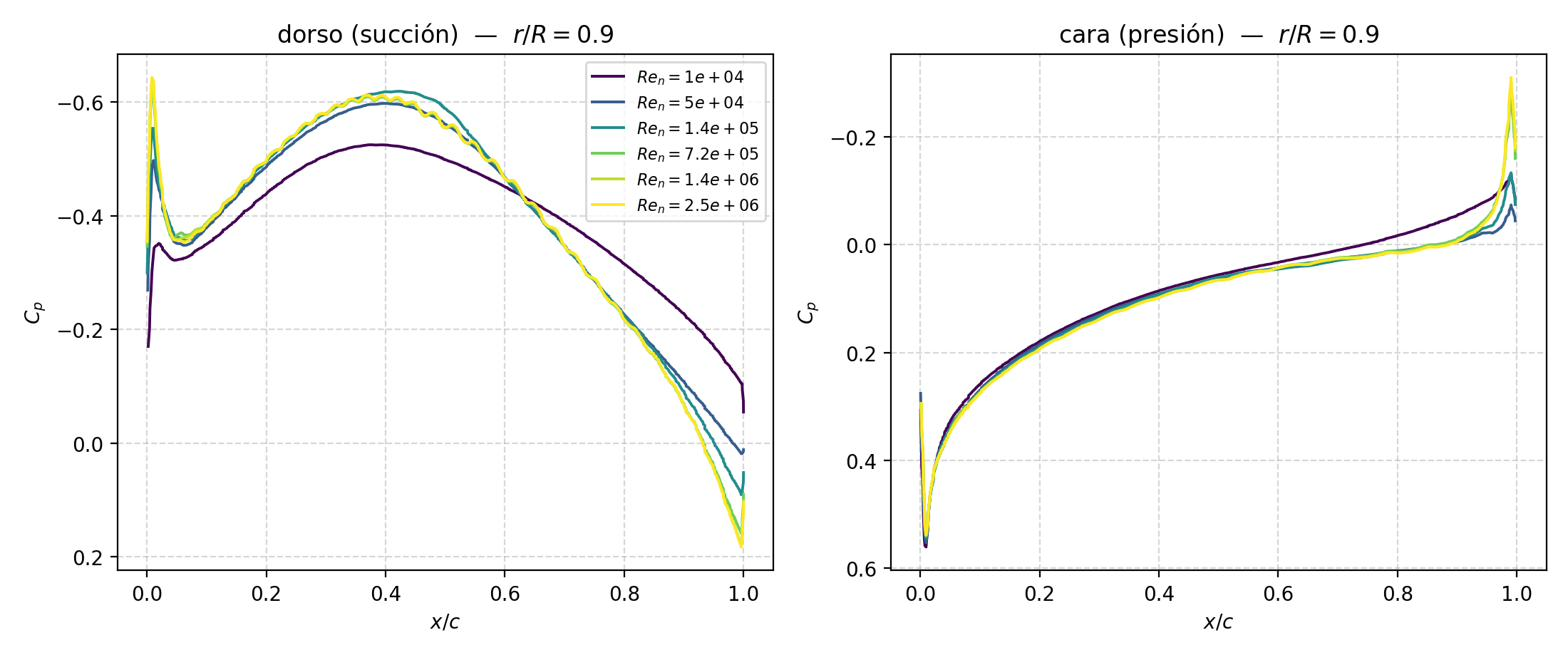
\includegraphics[width=\linewidth]{cp_section_r09.png}\\
  \small $C_p$ en $r/R=0.9$
\end{columns}
\end{frame}

\begin{frame}{Respaldo · \Pdos: robustez entre solvers}
\begin{columns}[T]
\column{0.49\textwidth}
  \centering
  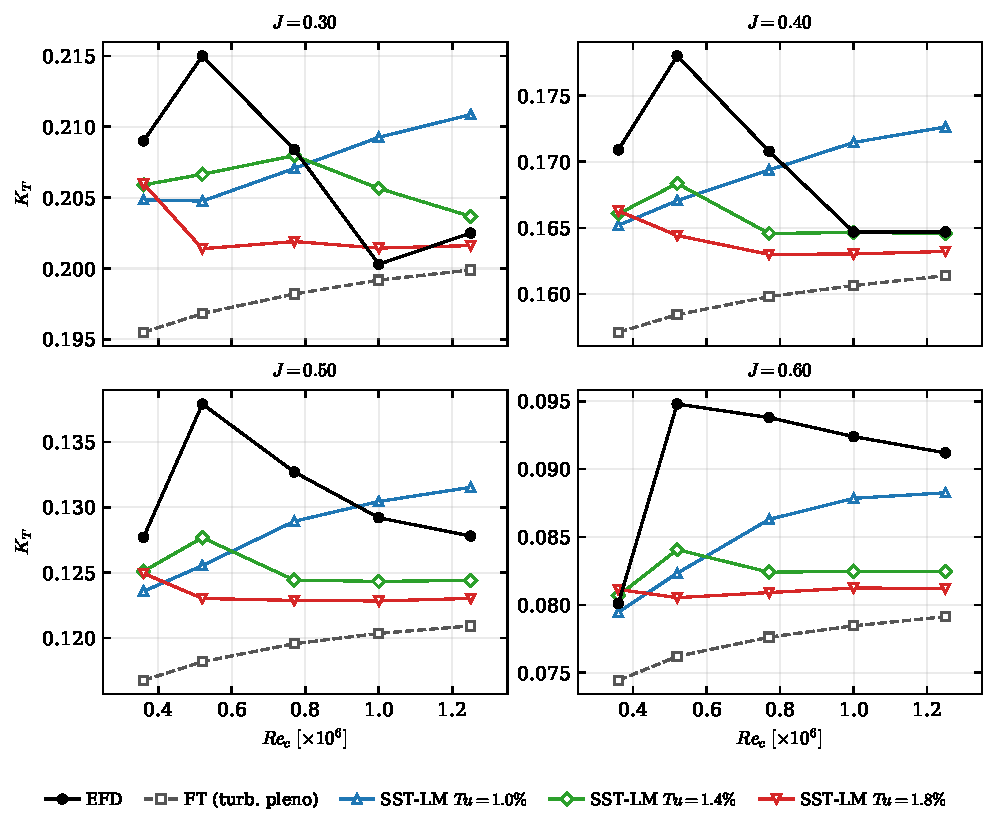
\includegraphics[width=0.88\linewidth]{fig_coreana_KT_OF.pdf}\\
  \small OpenFOAM
\column{0.49\textwidth}
  \centering
  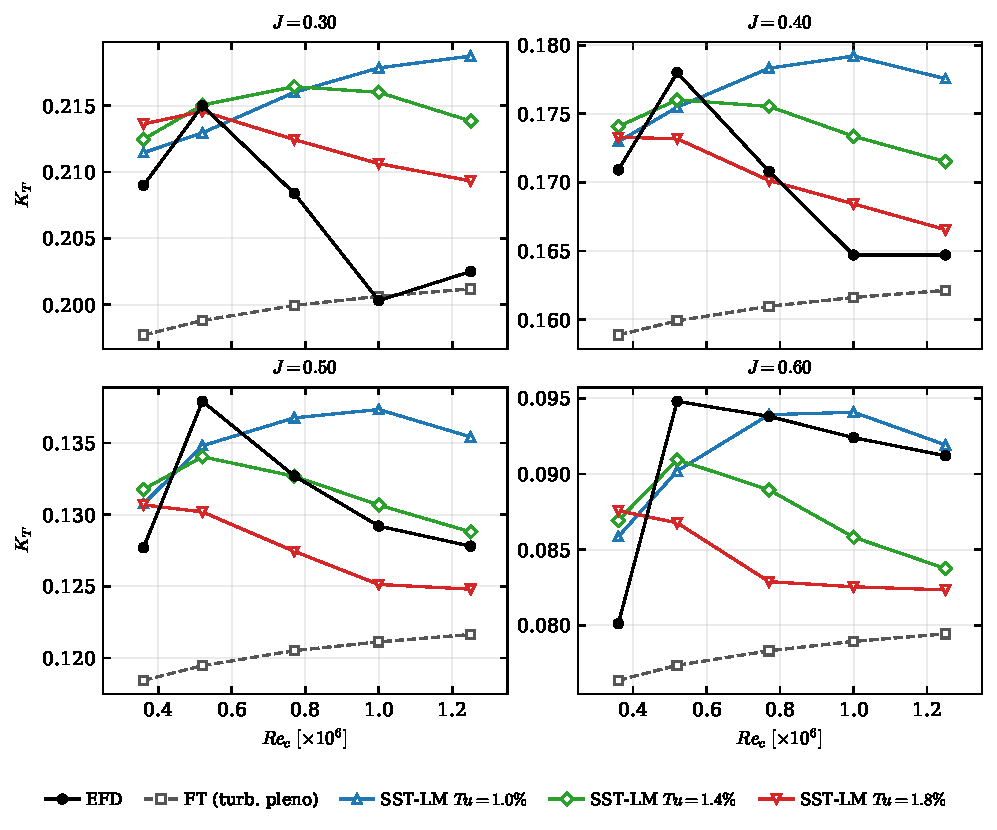
\includegraphics[width=0.88\linewidth]{fig_coreana_KT_Star.pdf}\\
  \small StarCCM+
\end{columns}
\vspace{0.4em}
\small La superioridad del SST-LM sobre el completamente turbulento es robusta entre solvers; la calibración fina de $Tu$ no lo es.
\end{frame}

\begin{frame}{Respaldo · \Pdos: distribución de $C_f$ sobre el dorso}
\begin{columns}[c]
\column{0.40\textwidth}
  \centering
  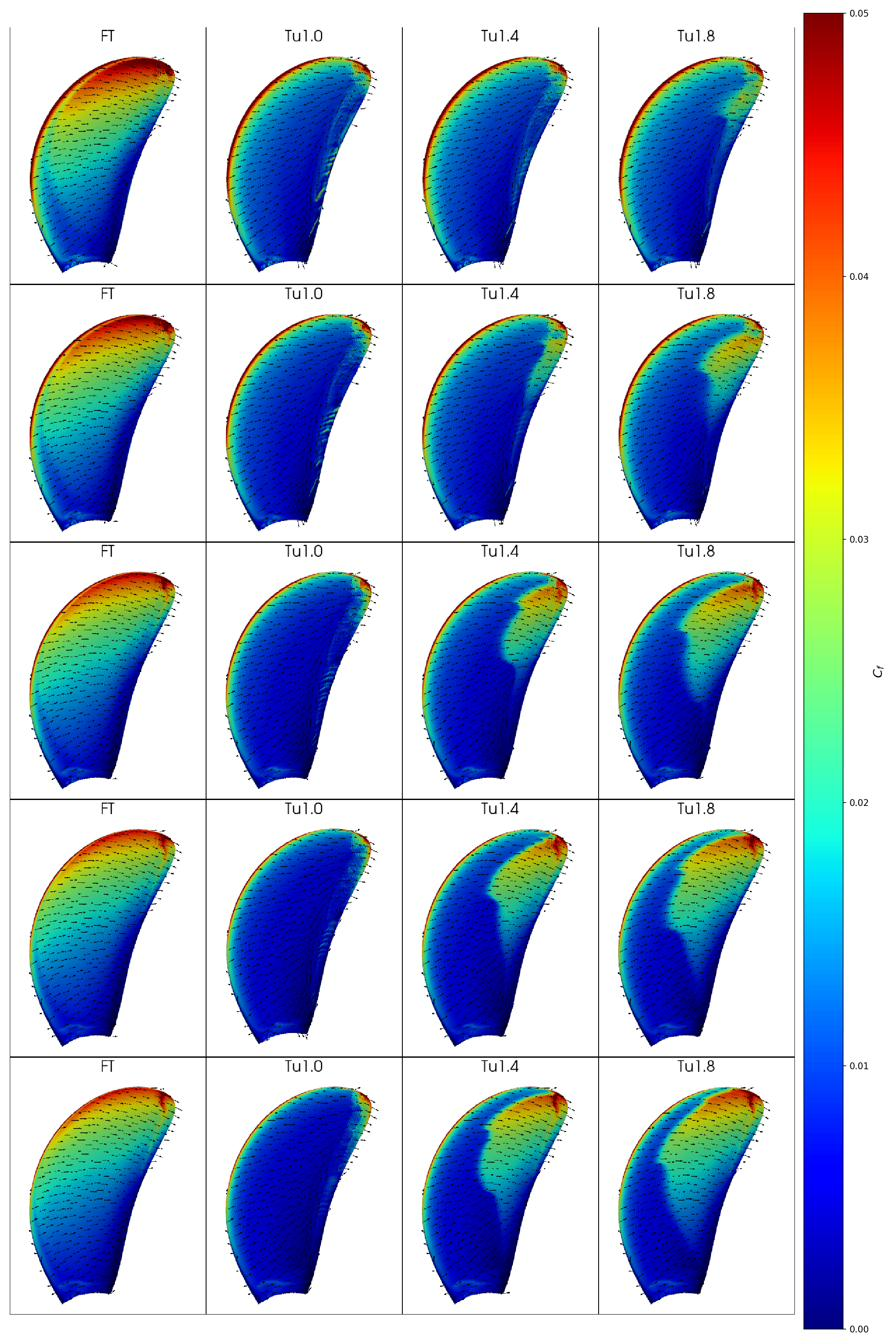
\includegraphics[height=5.5cm]{fig_cf_panel.png}
\column{0.58\textwidth}
  \begin{itemize}\small
    \item Frente de transición dependiente de $Tu$.
    \item Fracción radial de la tensión de corte: 0.19 (completamente turbulento) $\rightarrow$ 0.40–0.43 (SST-LM).
    \item Consistente con el mecanismo inferido de los “paint tests”.
  \end{itemize}
\end{columns}
\end{frame}

\end{document}
